\chapter{Results\label{cha:results}}

In the following chapter, the achieved results of the concept are presented. The described approaches are evaluated with regards to the common metrics precision, recall, and F1-Score. Different hyperparameter setups are discussed and visualised in graphs. In particular, the language models Bert, XL-Transformers and GPT-2 as described in \ref{transformer-approach} are compared. Additionally, the regression-based method as described in \ref{sec:regression} and the multi-classification method as described in \ref{sec:classification} are compared, showing advantages or disadvantages among each other.


\section{Experimental Setup}
The machine that was used to conduct the experiments has the following specifications:
\begin{itemize}
	\item Intel(R) Core(TM) i5-9600K CPU @ 3.70GHz
	\item 128 GB RAM
	\item 2 x NVIDIA GeForce RTX 2080 Ti 11GB RAM
	\item Ubuntu 18.04.3 LTS
\end{itemize}

\noindent The most relevant libraries that were used, with their corresponding versions can be seen in the following list:
\begin{itemize}
	\item Python 3.6.7
	\item Numpy 1.14.5
	\item PyTorch 1.4.0
	\item Transformers 2.3.0
	\item Tensorflow 2.1.0
\end{itemize}

\noindent The word embedding vector of the used language models have the following dimensions:
\begin{itemize}
	\item Bert: 768 
	\item GPT-2: 768
	\item XL-Transformers: 1024
\end{itemize}

\subsection{Anomaly Detection on one Dataset \label{sec:ad_one_ds_result}}
For evaluating the model, the OpenStack datasets "normal log dataset 2" (referenced to as original dataset from now on) containing 137k log lines and the "log dataset having performance anomalies" containing 18k log lines (referenced to as test dataset from now on), provided by the DeepLog authors at the University of Utah are used \cite{utah_dataset}. The original dataset stems from logs from running multiple OpenStack instances for 20 hours and 13 minutes for the original dataset and 2 hours and 17 minutes for the test dataset on CloudLab \cite{cloudlab}. Since the test dataset contains anomalies which are only detectable by inspecting the parameters of the log events, as described in \ref{fig:parsing}, i.e. the variable part of the log event which is not visible in the template after parsing, anomalies are injected into the dataset, yielding a labeled dataset for testing. This is necessary due to the assumptions specified in \ref{sec:requirements_and_assumptions}.
In order to assess the quality of the used word embeddings, log alterations are additionally injected into the dataset containing anomalies, in order to simulate the instability of logs as described in \ref{sec:logs_alteration}.


\subsection{Transfer Learning \label{sec:transfer_learning_setup}}
In order to examine the ability of the model to transfer the knowledge obtained from one dataset to a different one, the same OpenStack log dataset as utilised in \ref{sec:ad_one_ds_result} is used as a basis. First, on the basis of the templates which are presented in table \ref{tab:templates_after_cleansing}, the templates which are all altered throughout the dataset can be seen in \ref{fig:transfer_modifications}, in order to simulate a different dataset. Additionally, various of the alterations discussed in \ref{sec:logs_alteration} are injected all at once. For the following experiments, line shuffling, duplication and deletion, and word insertion, removal and replacement are injected into the dataset at various ratios in dataset A. The model is then trained on this dataset A for 60 epochs. As dataset B, the unaltered version of dataset A is then used to conduct few-shot training on the model, followed by anomaly detection on a dataset that has the same characteristics as B, i.e. no alterations.

\begin{figure}[H]
  \centering
  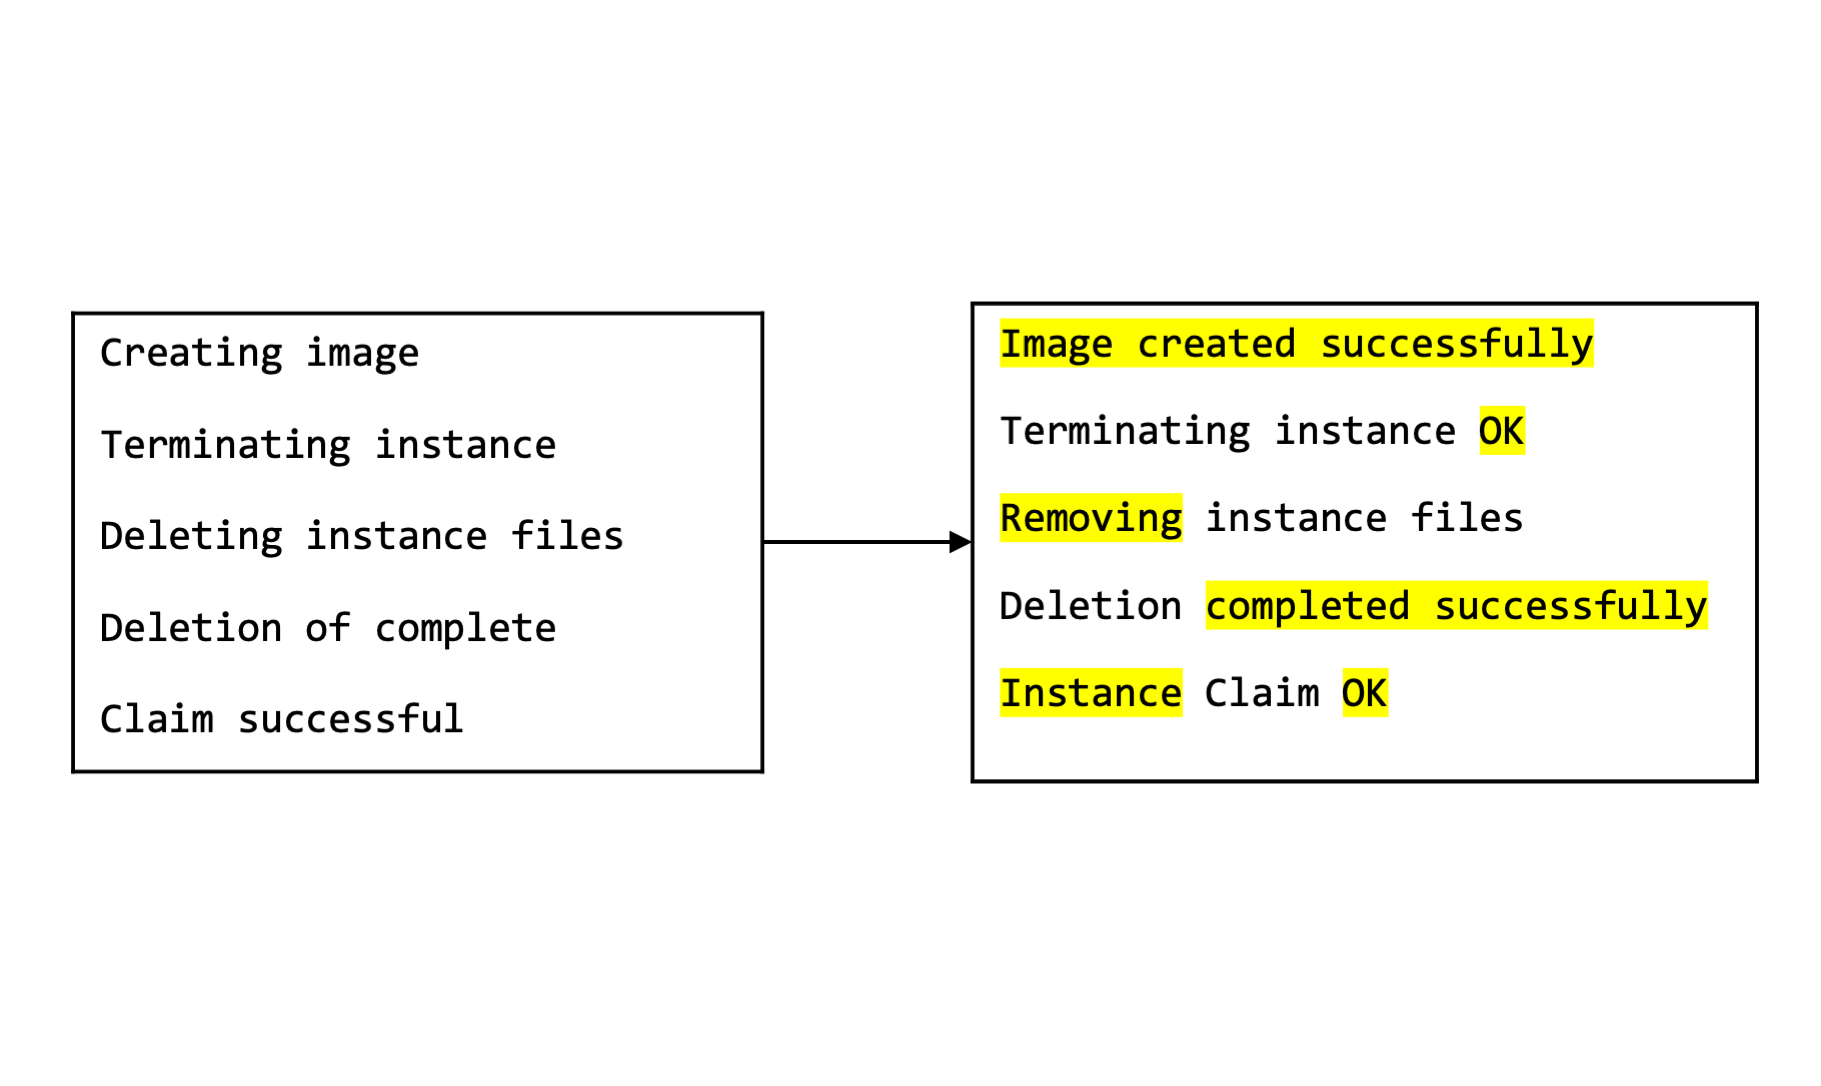
\includegraphics[width=10cm,height=6cm]{transfer_modifications.png}\\
  \caption{Changes on templates of the original dataset.}
  \label{fig:transfer_modifications}
\end{figure}




\section{Evaluation}
\subsection{Pre-Processing}
\subsubsection{String cleansing}
String cleansing, as described in \ref{sec:template_cleansing}, can potentially  improve distinguishability between templates drastically in the used dataset.
For Bert, the pairwise cosine distances before cleansing are depicted in figure \ref{fig:bert_before_cleansing}, after cleansing in figure \ref{fig:bert_after_cleansing}. The corresponding templates to the indices on the x and y axes before and after cleansing can be found in table \ref{tab:templates_before_cleansing} and table \ref{tab:templates_after_cleansing} respectively.
The cosine distances before and after cleansing for GPT-2 can be found in figure \ref{fig:gpt_before_cleansing} and figure \ref{fig:gpt_after_cleansing}, and for XL-Transformer in figure \ref{fig:xl_before_cleansing} and figure \ref{fig:xl_after_cleansing}, respectively. The average pairwise cosine distances between templates before and after cleansing can be seen in table \ref{tab:average_pairwise_cos_distances}.
Note that the cosine distances between templates appear to be relatively low for GPT-2 before and after cleansing. Even though cleansing results in a two-fold increase in the distances, the initial value is already very low. We can see how the distinguishability between templates increases for Bert and even more impressively for XL-Transformers. While Bert has a slightly higher average pairwise cosine distance before cleansing, XL-Transformers highly benefits from cleansing with an average value of 0.62. This underlines the importance of this step in order to meet the requirements postulated in \ref{sec:word_vectorization}, depending on the deployed language models.



\begin{table}[ht]
\centering
\begin{small}
\begin{tabular}{ p{1.3cm} p{2.5cm} p{2.5cm} }
\toprule
Model & Before cleansing & After cleansing\\
\midrule
XL & 0.2232 & 0.6223\\
Bert & 0.2416 & 0.4449\\
GPT-2 & 0.0024 & 0.0047 \\ 

\bottomrule
\end{tabular}
\caption{Average pairwise template cosine distances.}
\label{tab:average_pairwise_cos_distances}
\end{small}
\end{table}


\begin{figure}[!tbp]
  \centering
  \subfloat[Before cleansing.]{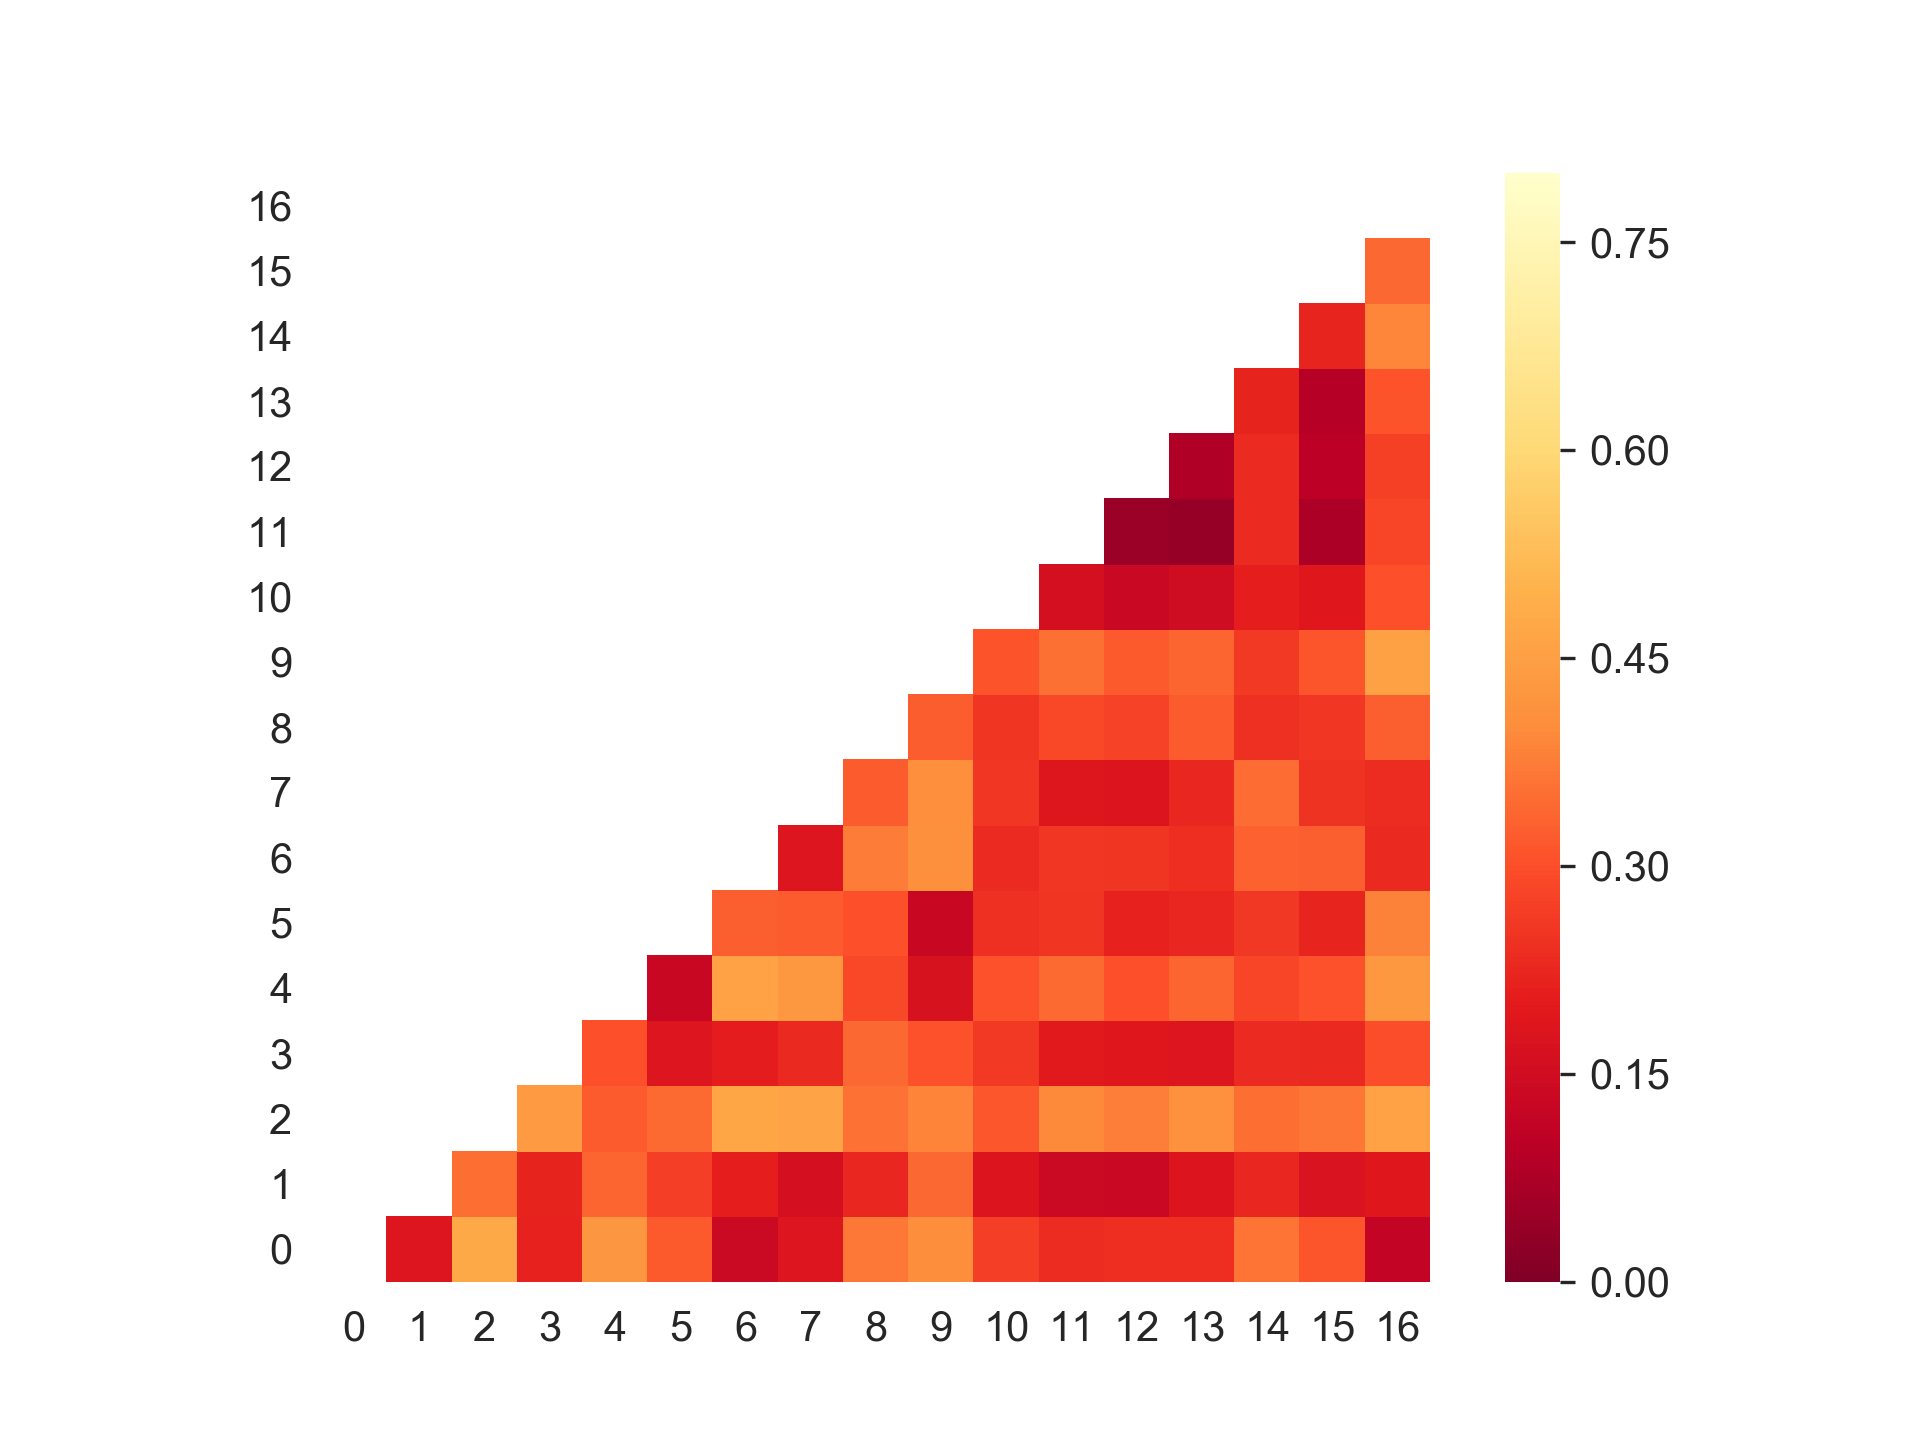
\includegraphics[width=0.5\textwidth]{bert_before_cleansing.png}\label{fig:bert_before_cleansing}}
  \hfill
  \subfloat[After cleansing.]{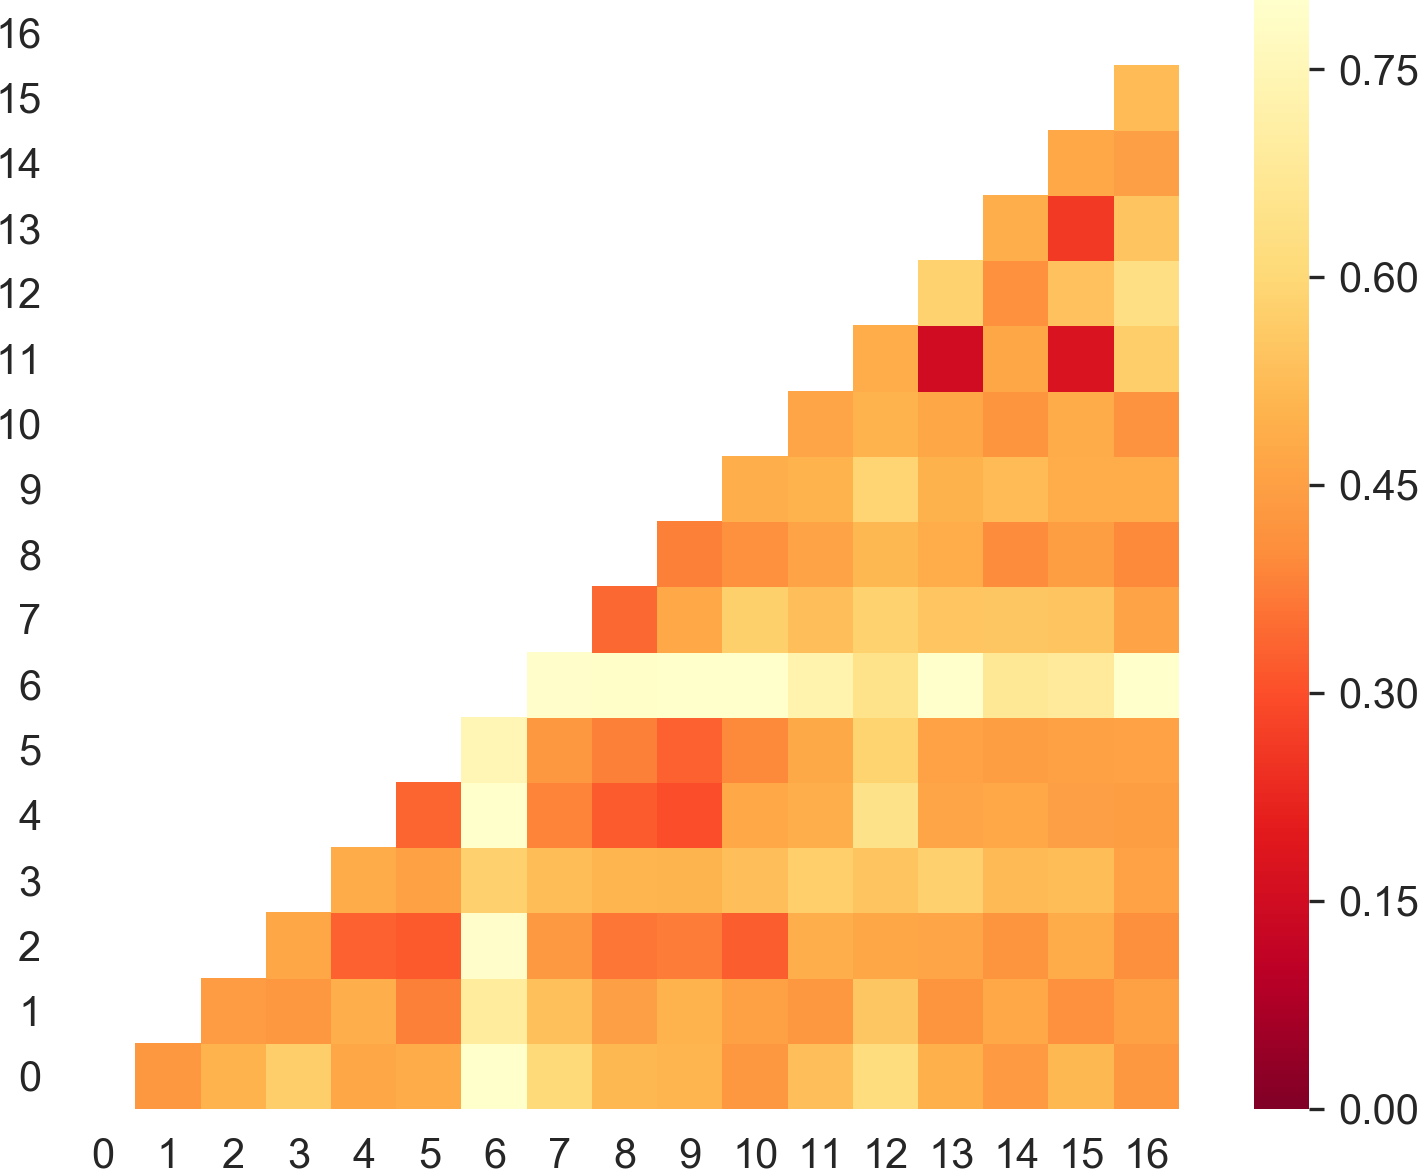
\includegraphics[width=0.5\textwidth]{bert_after_cleansing.png}\label{fig:bert_after_cleansing}}
  \caption{Bert pairwise template cosine distance.}
\end{figure}

\begin{figure}[!tbp]
  \centering
  \subfloat[Before cleansing.]{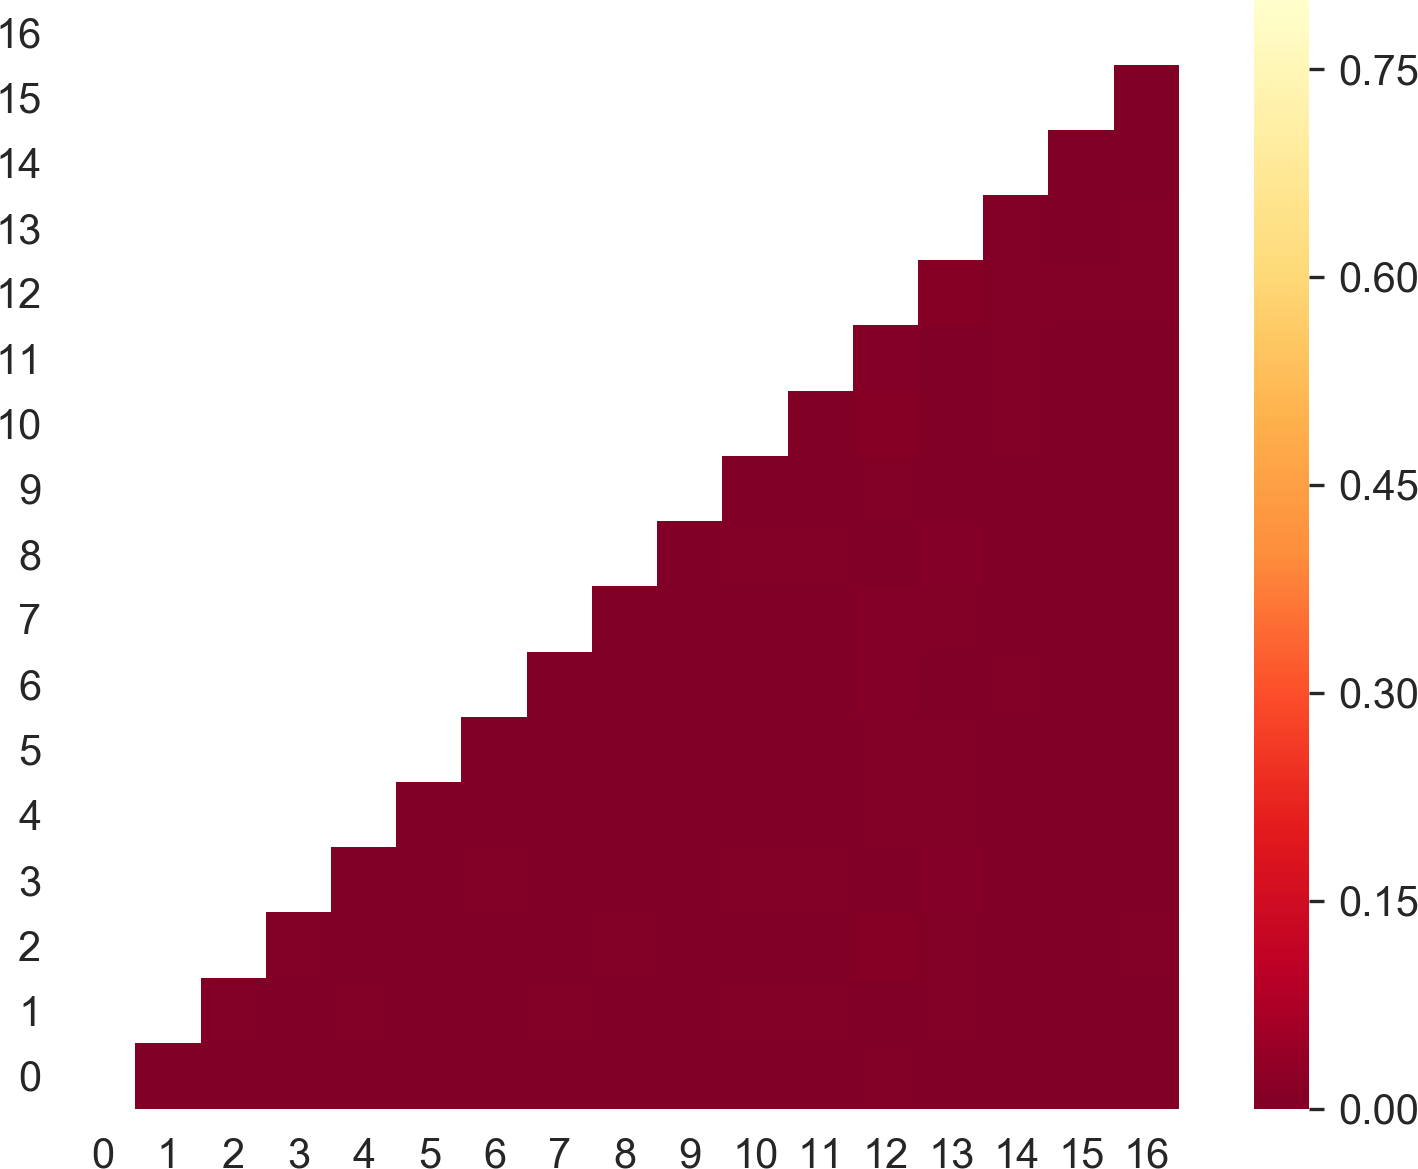
\includegraphics[width=0.5\textwidth]{gpt_before_cleansing.png}\label{fig:gpt_before_cleansing}}
  \hfill
  \subfloat[After cleansing.]{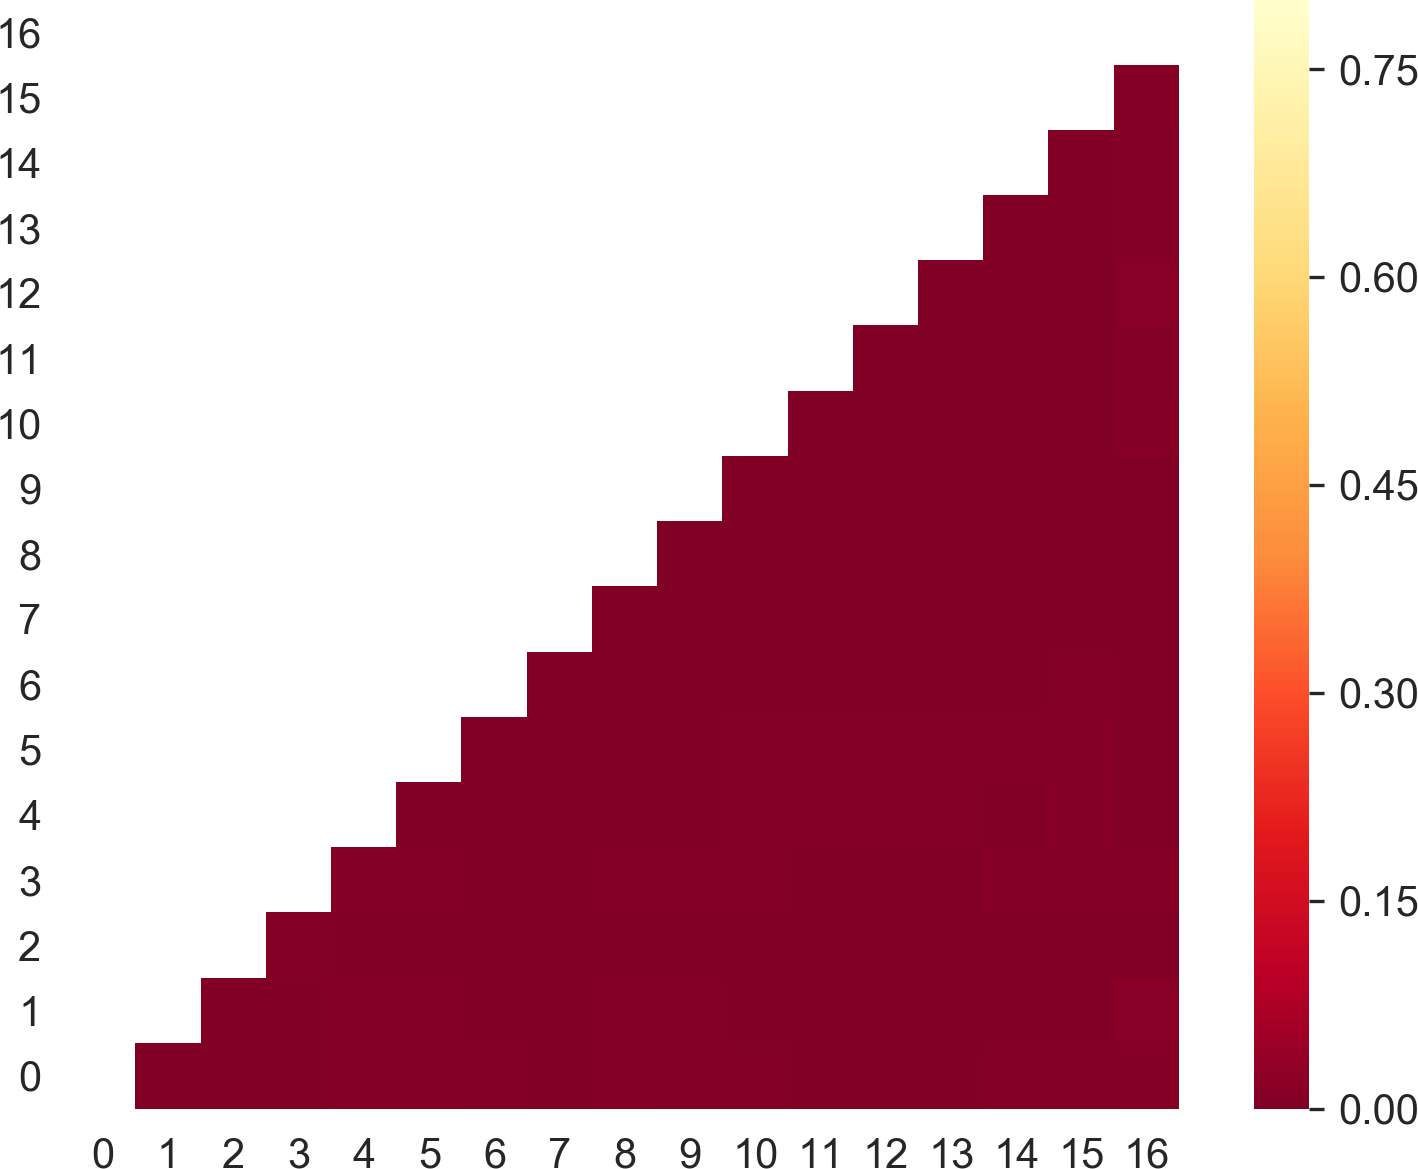
\includegraphics[width=0.5\textwidth]{gpt_after_cleansing.png}\label{fig:gpt_after_cleansing}}
  \caption{GPT-2 pairwise template cosine distance.}
\end{figure}

\begin{figure}[!tbp]
  \centering
  \subfloat[Before cleansing.]{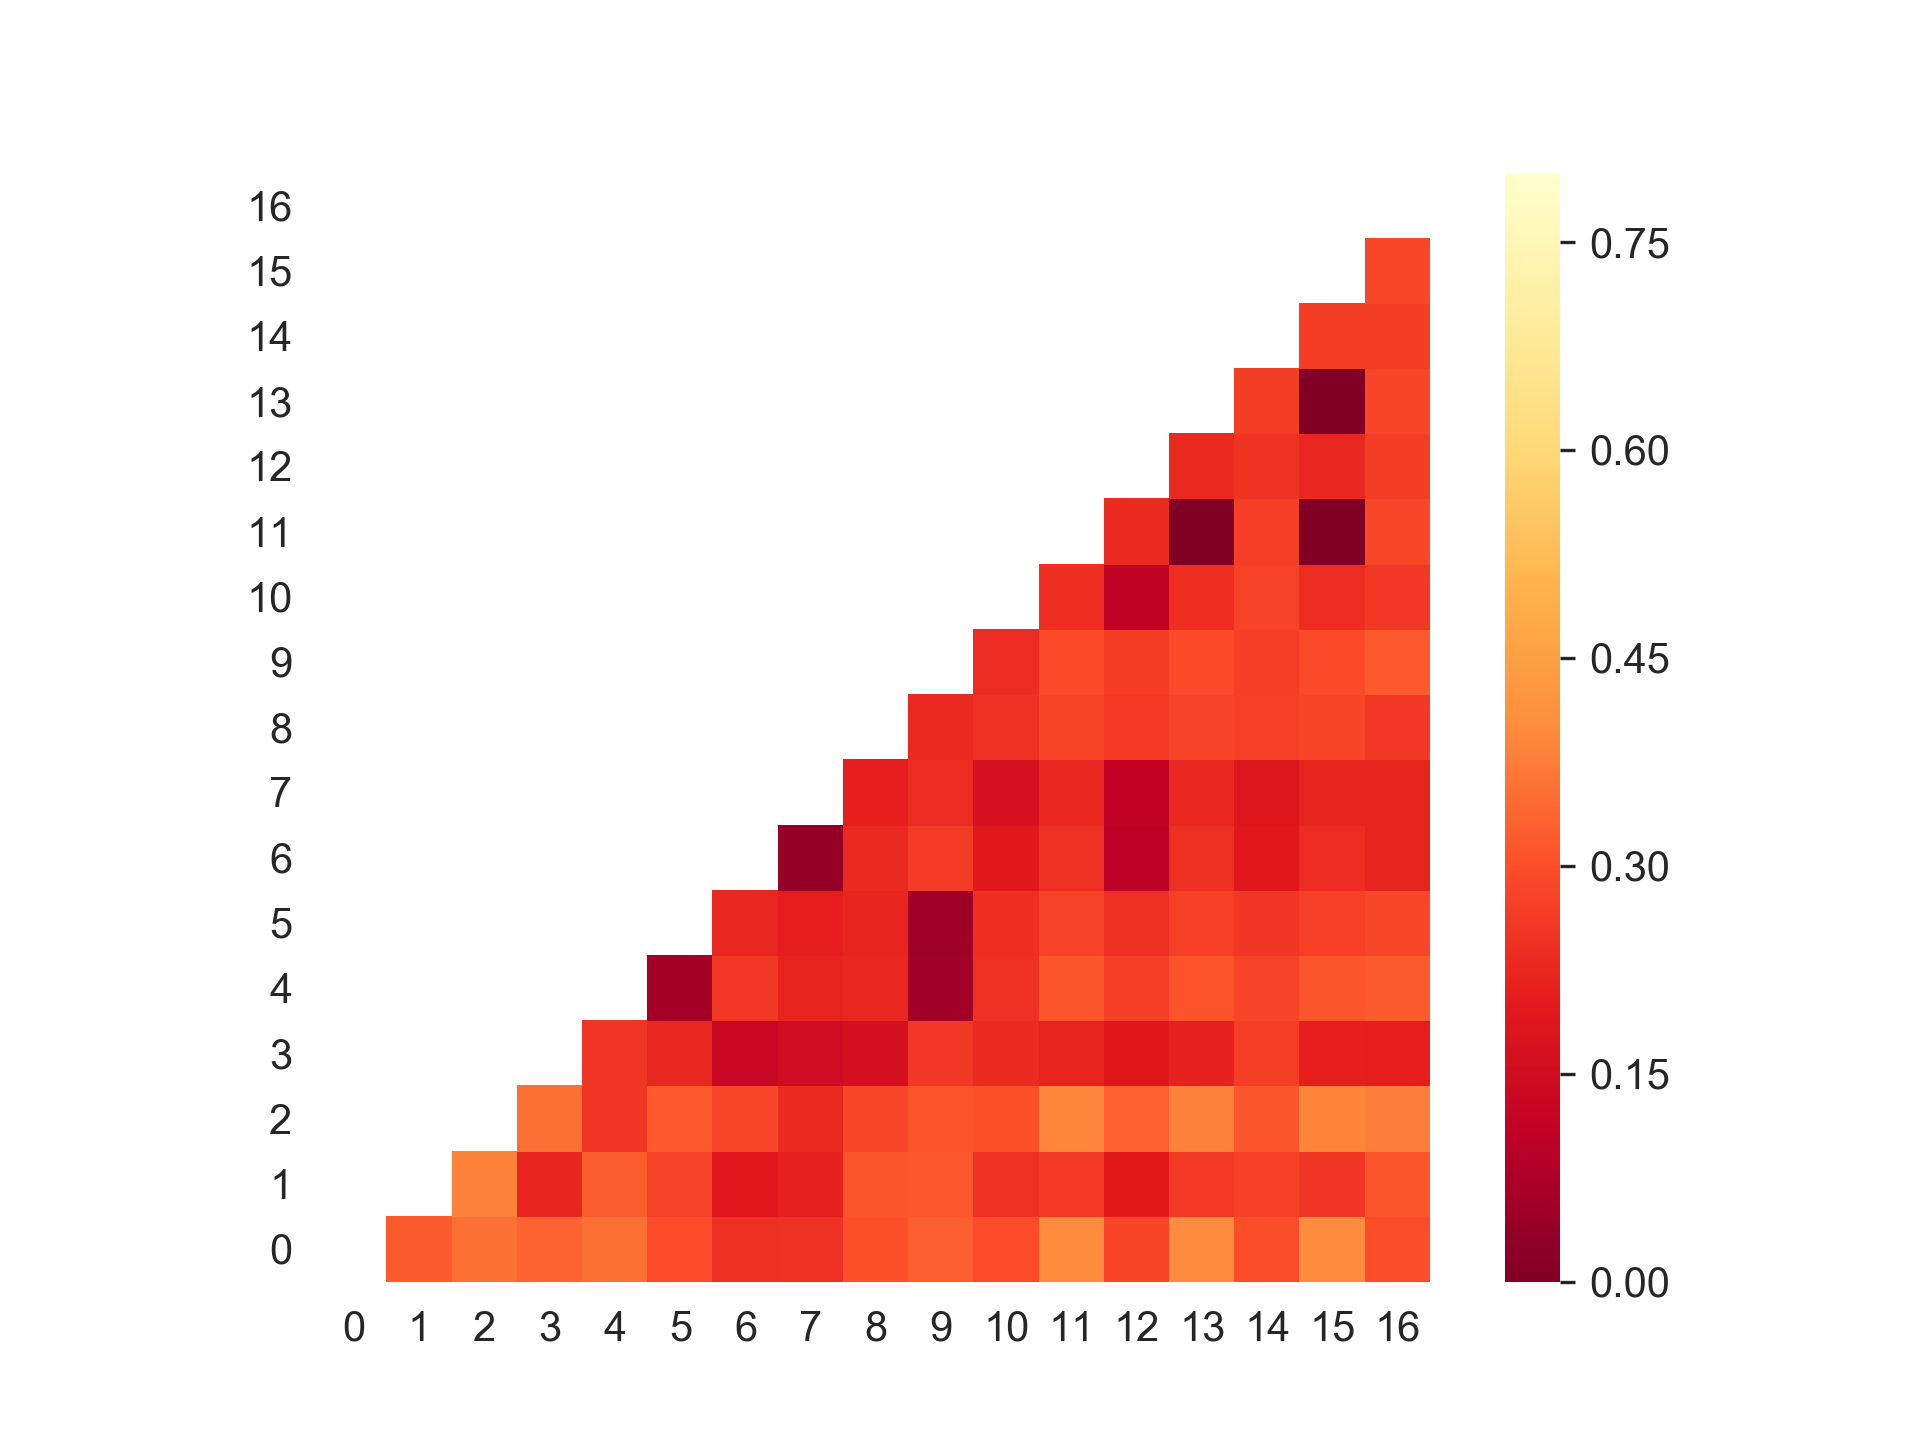
\includegraphics[width=0.5\textwidth]{xl_before_cleansing.png}\label{fig:xl_before_cleansing}}
  \hfill
  \subfloat[After cleansing.]{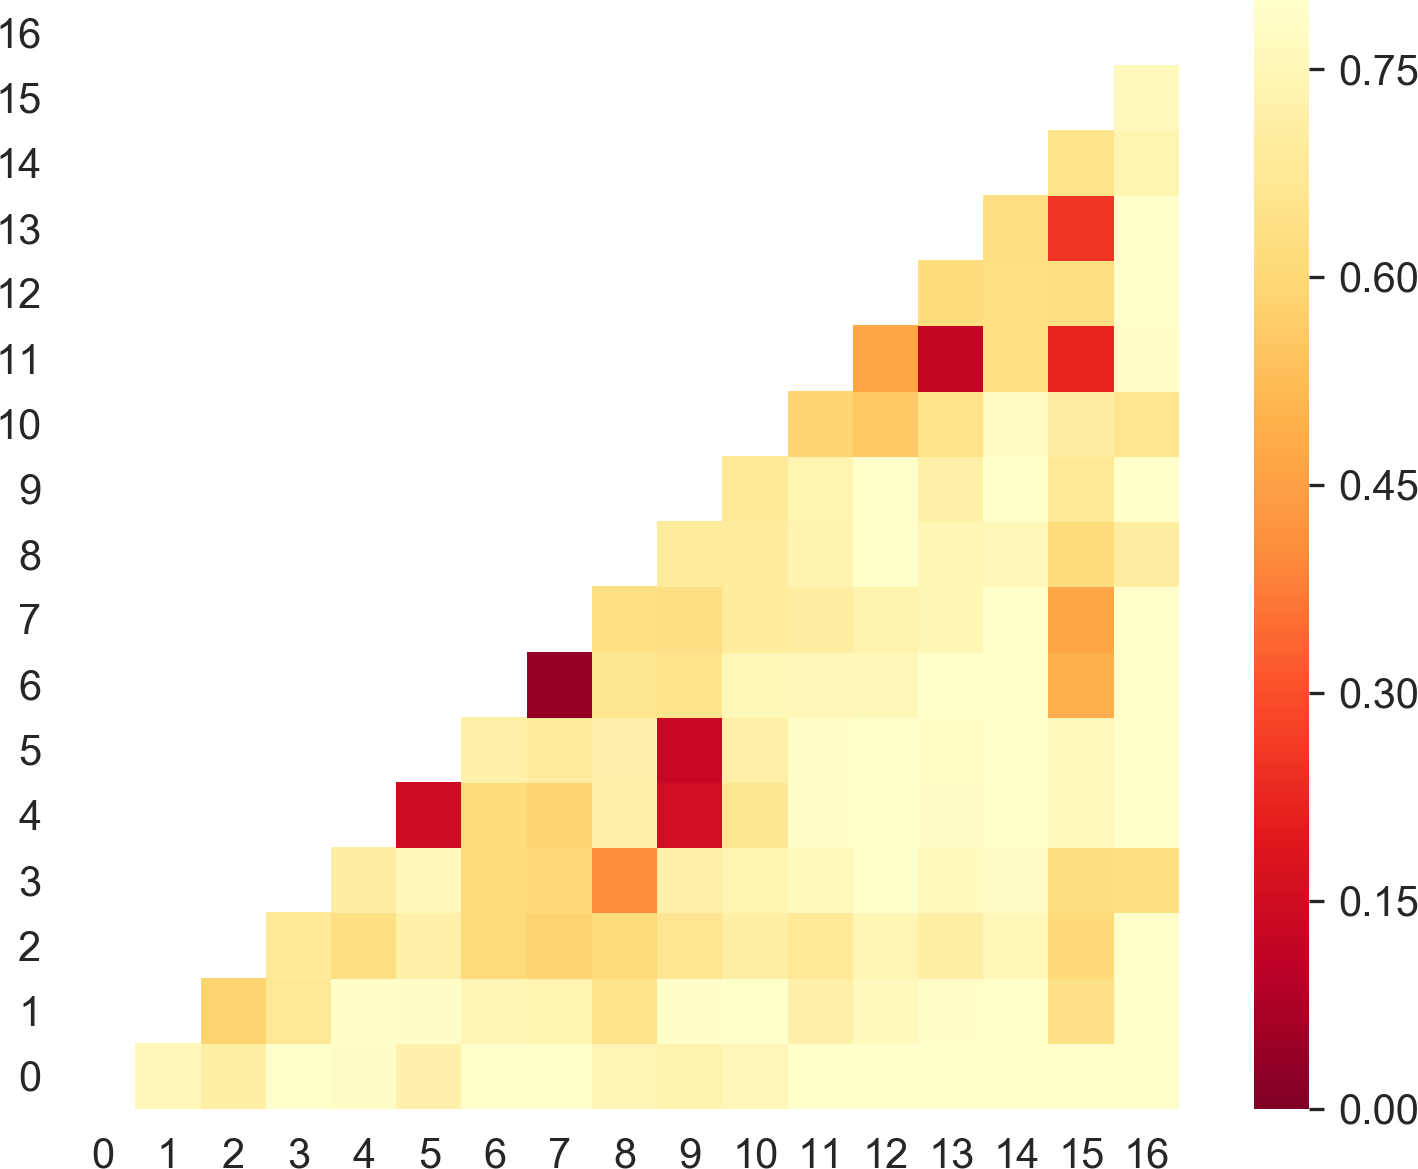
\includegraphics[width=0.5\textwidth]{xl_after_cleansing.png}\label{fig:xl_after_cleansing}}
  \caption{XL-Transformers pairwise template cosine distance.}
\end{figure}




\begin{table}[ht]
\begin{small}
\centering
\begin{tabular}{ c l } 
\toprule
Index & Template \\
\midrule
0 & $\langle*\rangle$ Creating image\\
1 & $\langle*\rangle$ VM $\langle*\rangle$ (Lifecycle Event)\\
2 & $\langle*\rangle$ During sync\_power\_state the instance has a pending task (spawning). Skip.\\
3 & $\langle*\rangle$ Instance $\langle*\rangle$ successfully.\\
4 & $\langle*\rangle$ Took $\langle*\rangle$.$\langle*\rangle$ seconds to $\langle*\rangle$ the instance on the hypervisor.\\
5 & $\langle*\rangle$ Took $\langle*\rangle$.$\langle*\rangle$ seconds to build instance.\\
6 & $\langle*\rangle$ Terminating instance\\
7 & $\langle*\rangle$ Deleting instance files $\langle*\rangle$\\
8 & $\langle*\rangle$ Deletion of $\langle*\rangle$ complete\\
9 & $\langle*\rangle$ Took $\langle*\rangle$.$\langle*\rangle$ seconds to deallocate network for instance.\\
10 & $\langle*\rangle$ Attempting claim: memory $\langle*\rangle$ MB, disk $\langle*\rangle$ GB, vcpus $\langle*\rangle$ CPU\\
11 & $\langle*\rangle$ Total memory: $\langle*\rangle$ MB, used: $\langle*\rangle$.$\langle*\rangle$ MB\\
12 & $\langle*\rangle$ memory limit: $\langle*\rangle$.$\langle*\rangle$ MB, free: $\langle*\rangle$.$\langle*\rangle$ MB\\
13 & $\langle*\rangle$ Total disk: $\langle*\rangle$ GB, used: $\langle*\rangle$.$\langle*\rangle$ GB\\
14 & $\langle*\rangle$ $\langle*\rangle$ limit not specified, defaulting to unlimited\\
15 & $\langle*\rangle$ Total vcpu: $\langle*\rangle$ VCPU, used: $\langle*\rangle$.$\langle*\rangle$ VCPU\\
16 & $\langle*\rangle$ Claim successful\\
\bottomrule
\end{tabular}
\caption{Templates before cleansing}
\label{tab:templates_before_cleansing}
\end{small}
\end{table}



\begin{table}[ht]
\begin{small}
\centering
\begin{tabular}{ c l } 
\toprule
Index & Template \\
\midrule
0 & Creating image\\
1 & VM  Lifecycle Event\\
2 & During sync power state the instance has a pending task spawning Skip\\
3 & Instance  successfully\\
4 & Took  seconds to  the instance on the hypervisor\\
5 & Took  seconds to build instance\\
6 & Terminating instance\\
7 & Deleting instance files\\
8 & Deletion of complete\\
9 & Took  seconds to deallocate network for instance\\
10 & Attempting claim memory  MB disk  GB vcpus  CPU\\
11 & Total memory  MB used  MB\\
12 & memory limit  MB free  MB\\
13 & Total disk  GB used  GB\\
14 & limit not specified defaulting to unlimited\\
15 & Total vcpu  VCPU used  VCPU\\
16 & Claim successful\\
\bottomrule
\end{tabular}
\caption{Templates after cleansing}
\label{tab:templates_after_cleansing}
\end{small}
\end{table}

\subsubsection{Finetuning}
As described in \ref{sec:finetuning}, finetuning can potentially help to produce word embeddings that are more adequate for solving a certain task, it is thus desirable to produce word embeddings that help solving the task of anomaly detection better. As described in \ref{sec:word_vectorization}, a high cosine distance between semantically different templates is required. The dataset that consists of the templates in table \ref{tab:templates_after_cleansing} has been chosen for finetuning. Since the pre-trained language models at hand (namely \textit{bert-base-uncased} and \textit{gpt2}) have been trained on a large corpus, finetuning would also need to be executed on a sufficiently large corpus. Since this is not the case, the results of finetuning for a maximum of four epochs, as suggested by the Bert authors \cite{devlin2018bert}, does not yield the desired results. As it can be seen in figure \ref{fig:cos_distance_finetuning}, it was not possible to increase the cosine distances between templates on the task of Masked LM (as described in \ref{Bert}), compared to the cosine distances depicted in figure \ref{fig:bert_after_cleansing}. The average distance between templates dropped to 0.3016 from 0.4449. The fact that the loss on the evaluation part of the dataset is not decreasing adequately, as shown in figure \ref{fig:finetuning_loss}, shows that training on such a small corpus is not able to generalise well enough, which makes finetuning on the default learning task not useful in this case. Since the Huggingface Transformers library does not offer out of the box finetuning interfaces for GPT-2 and XL-Transformers on the same task as for Bert, they are not further investigated for finetuning.

\begin{figure}[H]
  \centering
  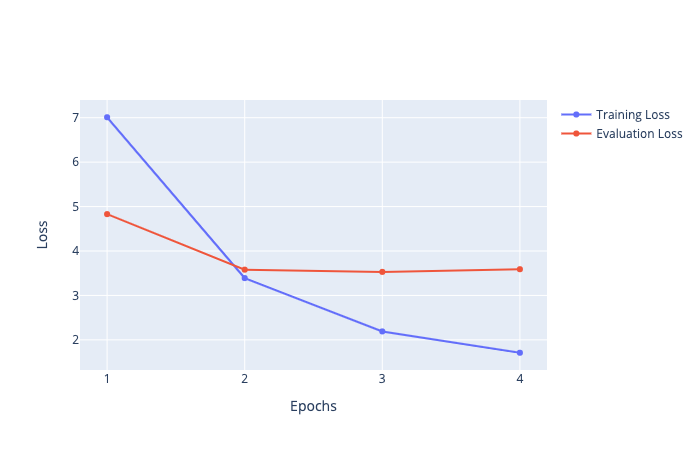
\includegraphics[width=12cm,height=8.5cm]{finetuning_loss.png}\\
  \caption{Training and evaluation loss for finetuning on masked LM.}
  \label{fig:finetuning_loss}
\end{figure}

\begin{figure}[h]
  \centering
  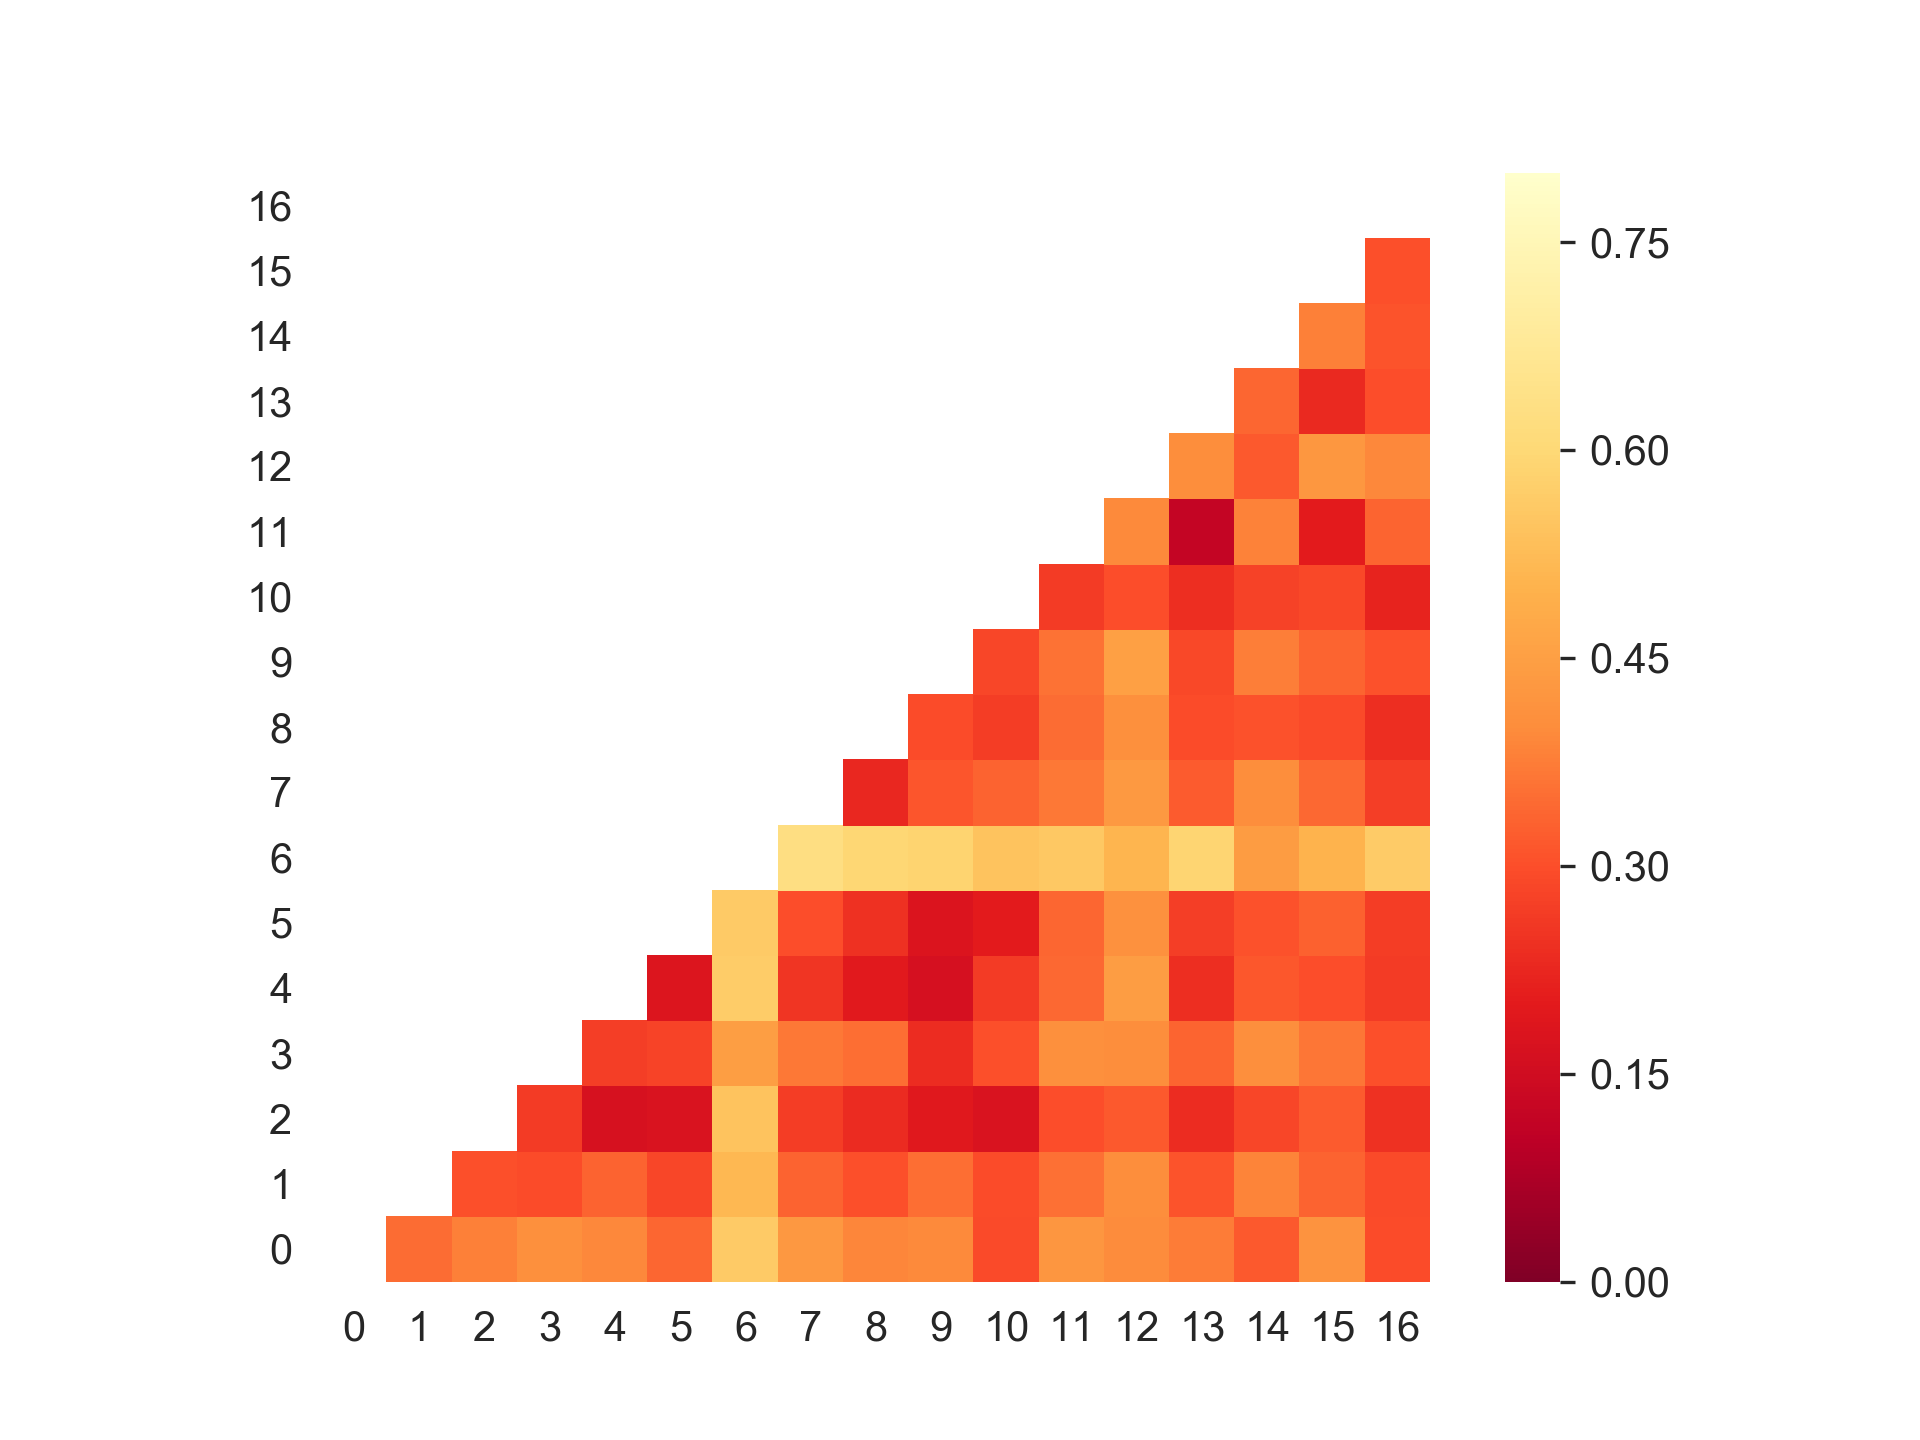
\includegraphics[width=12cm,height=9cm]{bert_finetuning_cleansed.png}\\
  \caption{Cosine distance between templates after cleansing and finetuning}
  \label{fig:cos_distance_finetuning}
\end{figure}


\subsubsection{Hyperparameters}
In order to find well-suited parameters for the LSTM model, it was first applied to the problem using a minimal configuration. With the help of a grid-search, running simulations with different configurations, the following hyperparameters have proven to yield the most satisfying results:
\begin{itemize}
	\item 512 hidden units for the bidirectional LSTM, with one layer
	\item two fully connected layers with 512 units $\rightarrow$ 256 units $\rightarrow$ output size
	\item dropout of 0.1 between every layer
	\item input sequence length of 7
	\item 60 Epochs of training
\end{itemize}

%%%%%%%%%%%%
% REGRESSION 
%%%%%%%%%%%%
\subsection{Evaluation of the regression-based approach using one dataset\label{sec:results-regression}}
In this subsection, the results of the regression-based approach, with various alterations using the different language models, are presented. In order to evaluate the robustness of the language models to the evolution of log events, alterations as described in \ref{sec:logs_alteration} are injected at different ratios. The impact on detecting injected anomalies after alterations on the sequence of logs are injected, i.e. deleting, shuffling and duplicating events are summarised in figure \ref{fig:results_regression_sequential}. Alterations are not injected all at the same time, but independently from each other, the results in the figures are average values of all experiments with alterations on the log sequences. Results broken down by each alteration can be found in the appendix \ref{appendix:regression}. It is evident, that GPT-2 performs better than Bert and XL-Transformers on both the F1-score and precision. Yet, when the \textit{reverse order} alteration is injected, which reverses all the log events per instance id block and therefore marks every line as an anomaly, in order to evaluate the ability of the model to learn sequences, the results are different. The metrics for this experiment are visualised in figure \ref{fig:regression_reverse_order}.

In contrast to the alterations on the log sequences, alterations on the log events themselves, i.e. inserting, removing and replacing words are also of interest. The results of this experiment can be seen in figure \ref{fig:results_regression_words}. Again, the alterations are not injected all at once, but independently - the figure shows averaged results.

Another aspect that is evaluated, is the impact of the input sequence length, i.e. the number of concatenated log events for which the next log event shall be predicted, on the ability of the model to detect anomalies. The results of this evaluation can be seen in \ref{fig:seq_len_regression}. Bert and GPT-2 seem to profit slightly from sequence lengths longer than 6 or 7, whereas the quality of results for XL-Transformers are not as affected from the input sequence length, but are generally lower.

\begin{figure}[h]
  \centering
  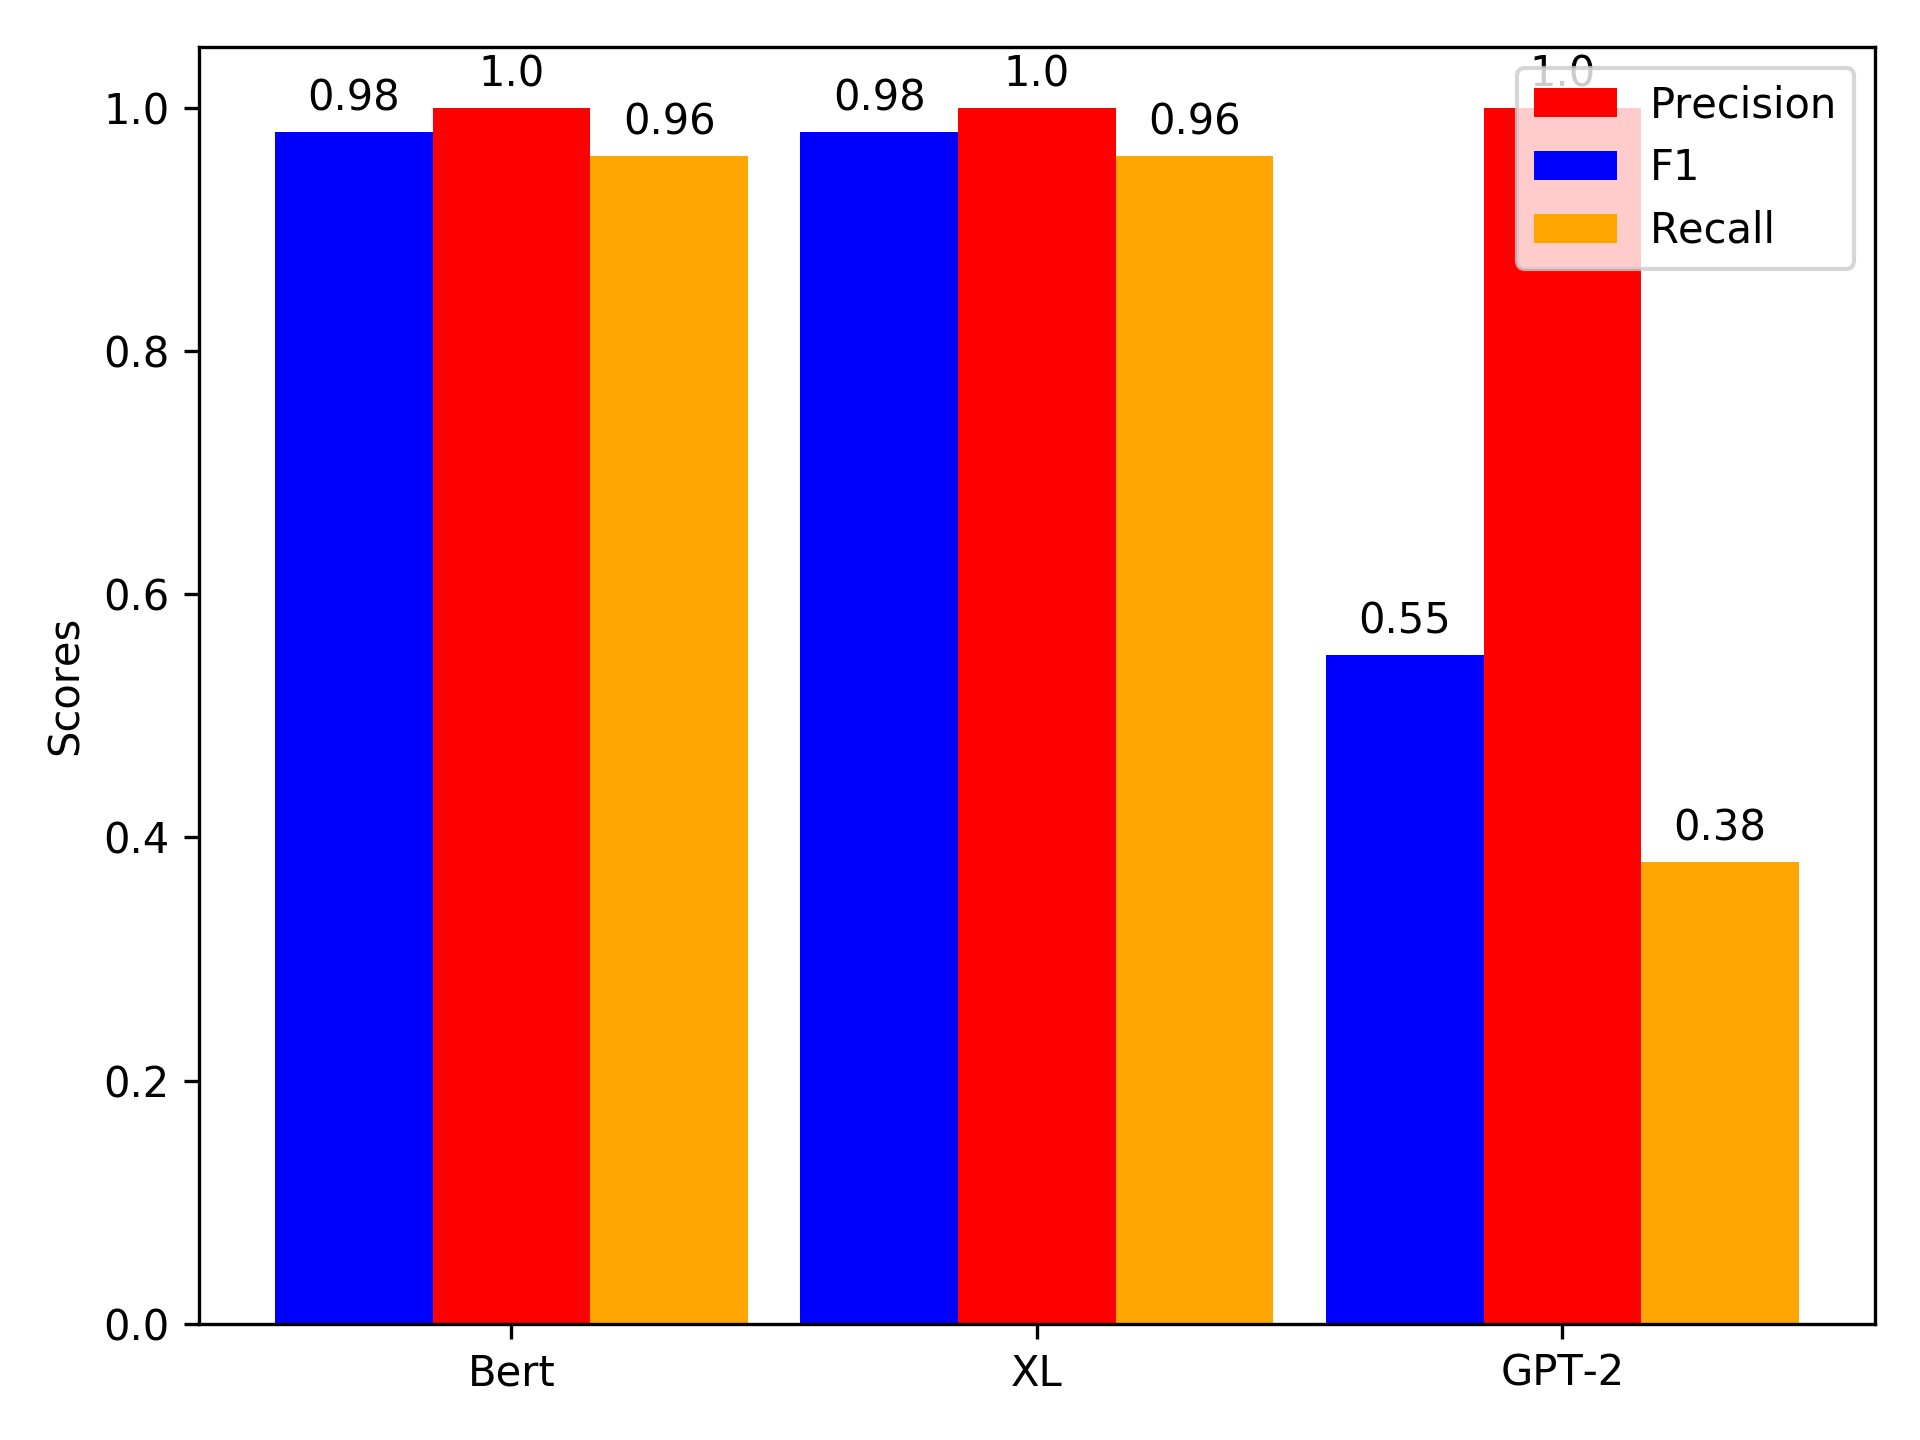
\includegraphics[width=6cm,height=4.5cm]{results/regression_sequence/regression_reverse.png}\\
  \caption{Scores for detecting reversed order of log events, using regression.}
  \label{fig:regression_reverse_order}
\end{figure}

\begin{figure*}[ht!]
   \subfloat[5\% alteration\label{fig:results_regression_sequential_5}]{%
      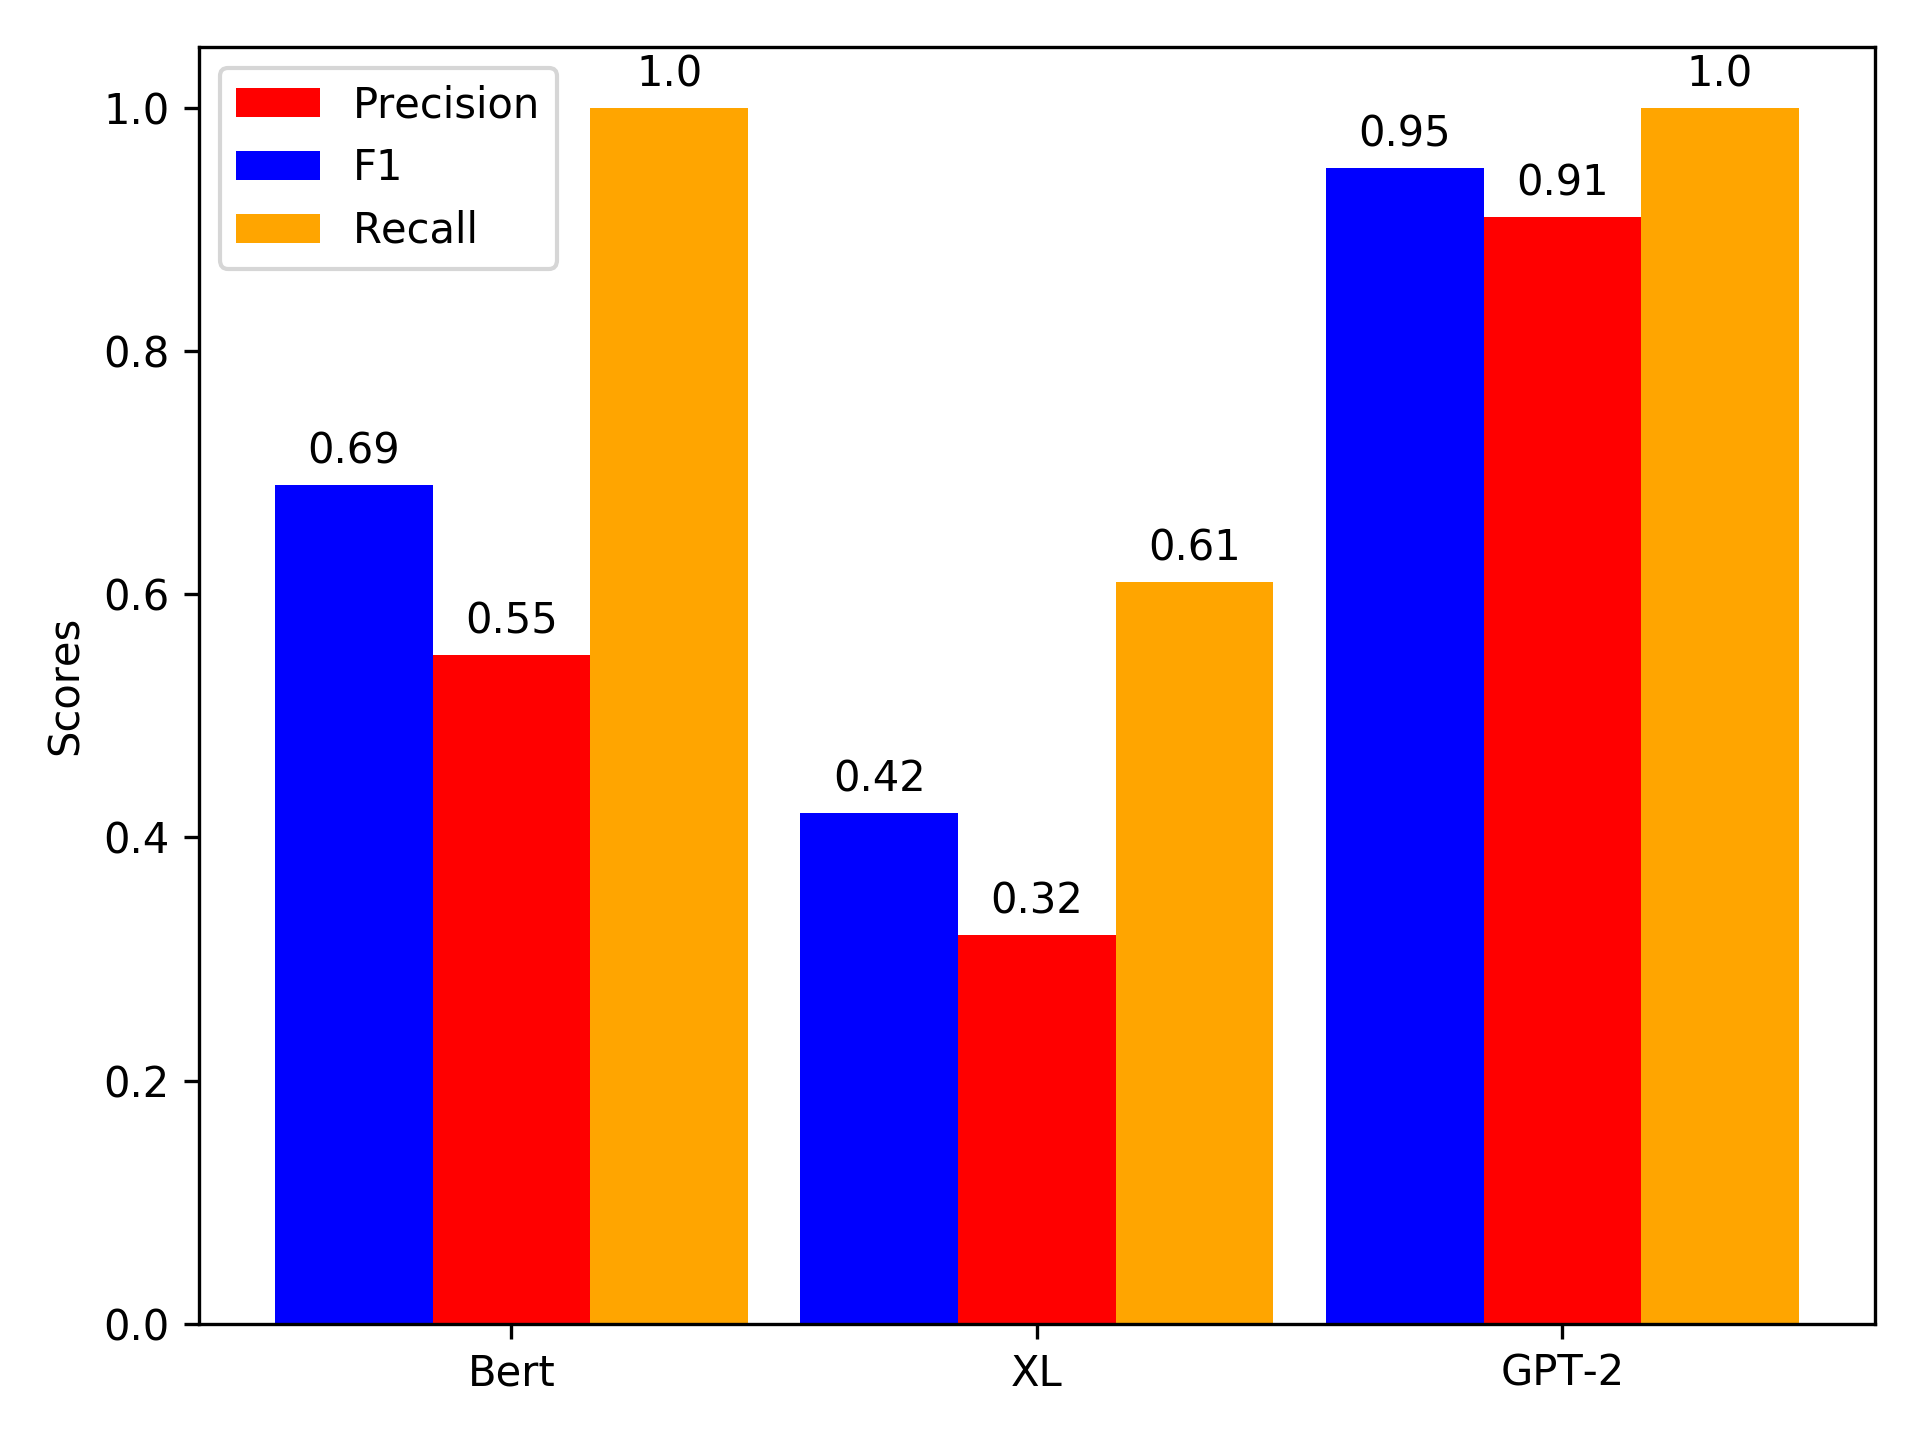
\includegraphics[trim={1cm 0.5cm 0cm 1cm}, width=0.322\textwidth]{results/average/regression_sequential_average_ratio_0.05.png}}
\hspace{\fill}
   \subfloat[10\% alteration\label{fig:results_regression_sequential_10} ]{%
      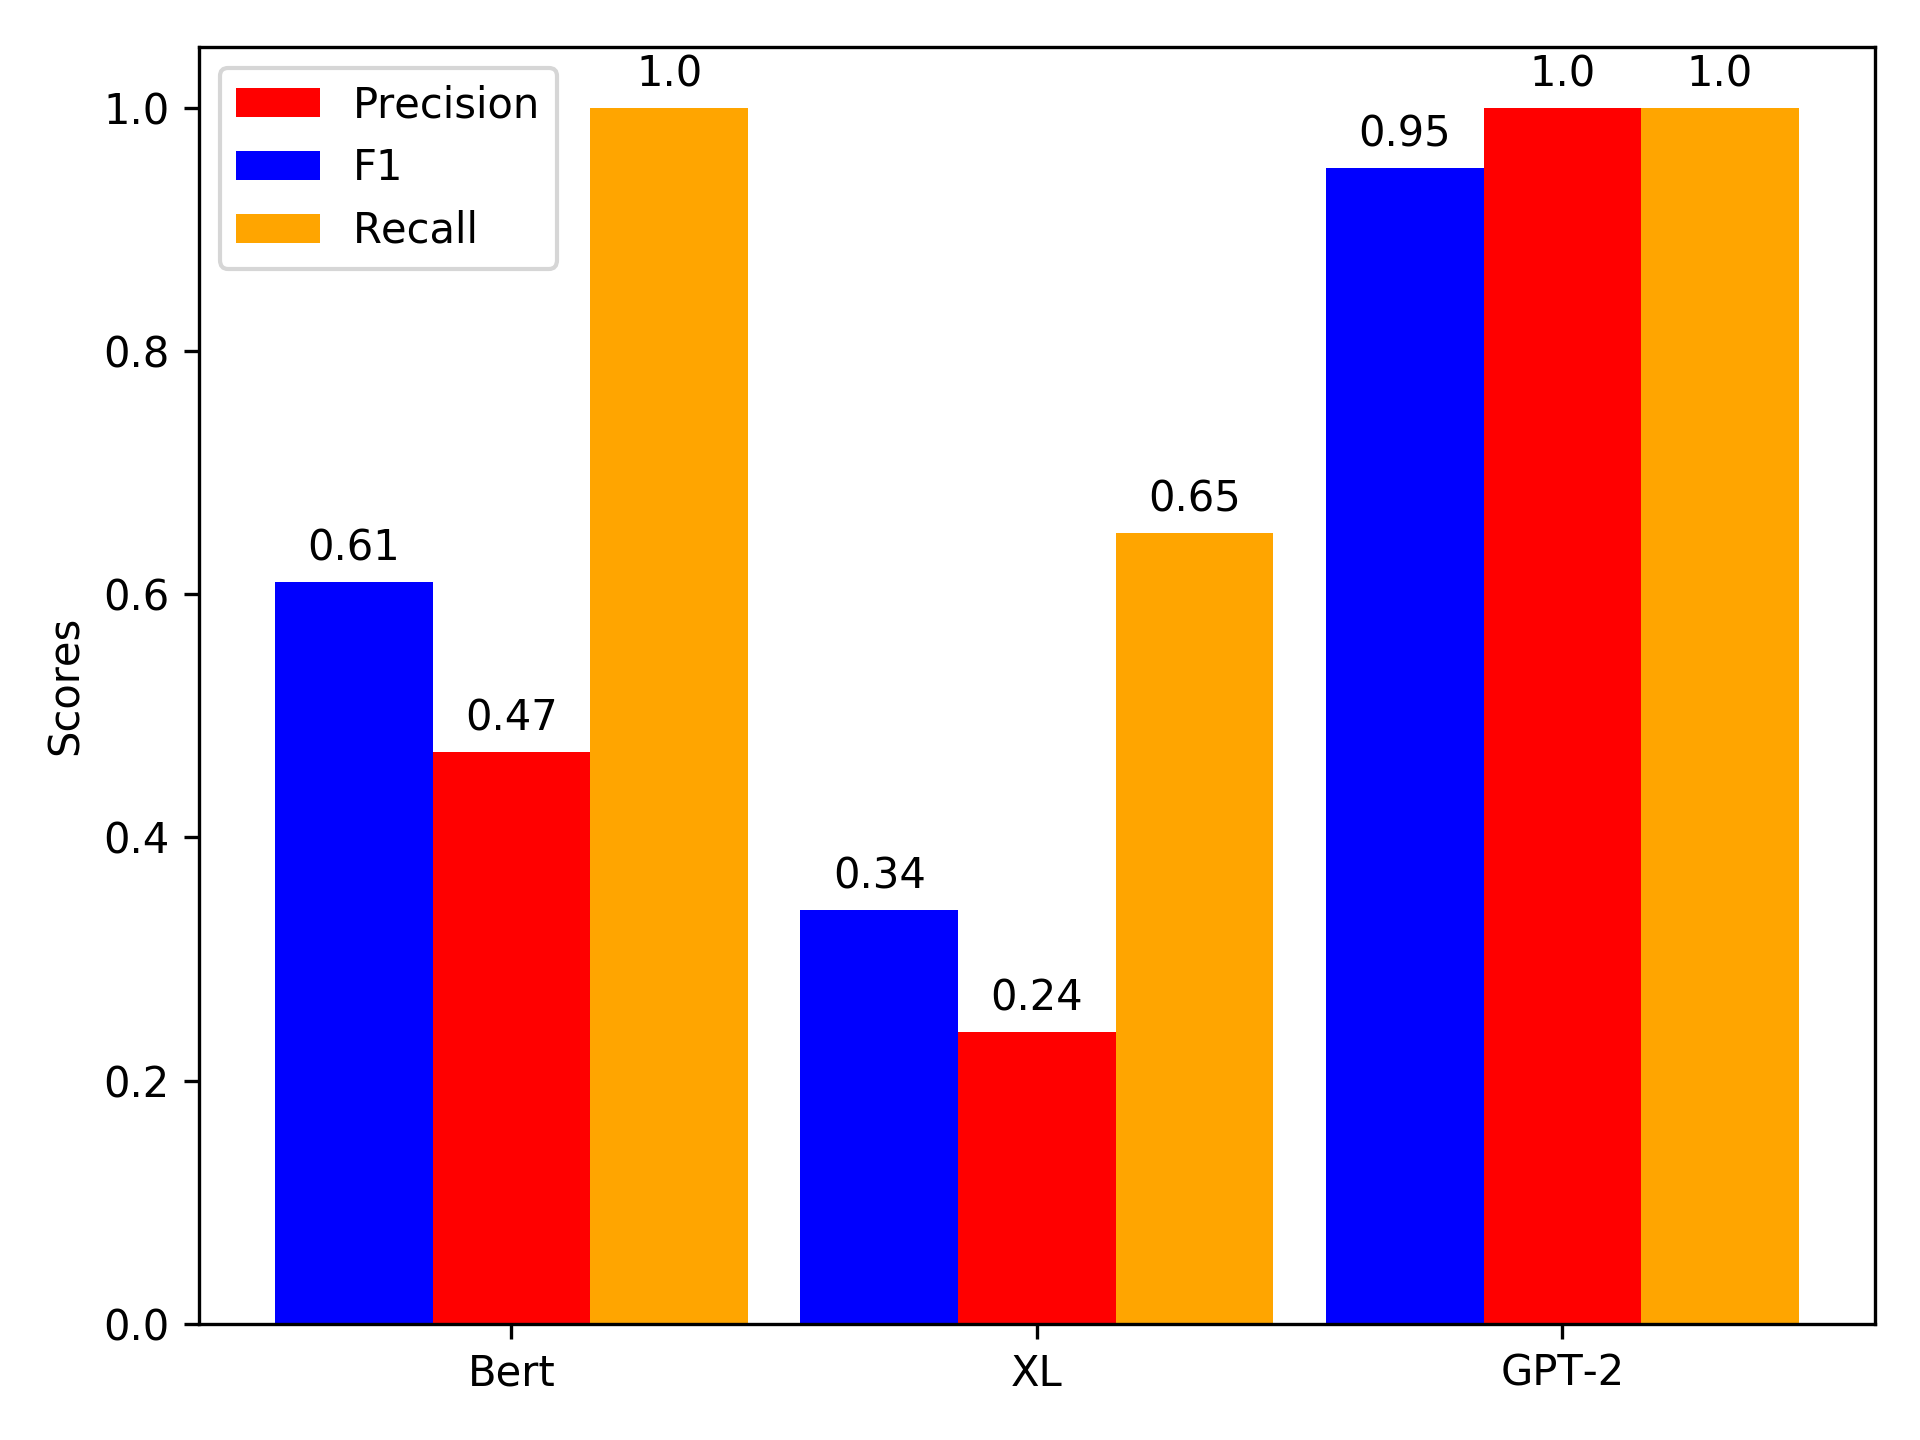
\includegraphics[trim={1cm 0.5cm 0cm 1cm}, width=0.322\textwidth]{results/average/regression_sequential_average_ratio_0.10.png}}
\hspace{\fill}
   \subfloat[15\% alteration\label{fig:results_regression_sequential_15}]{%
      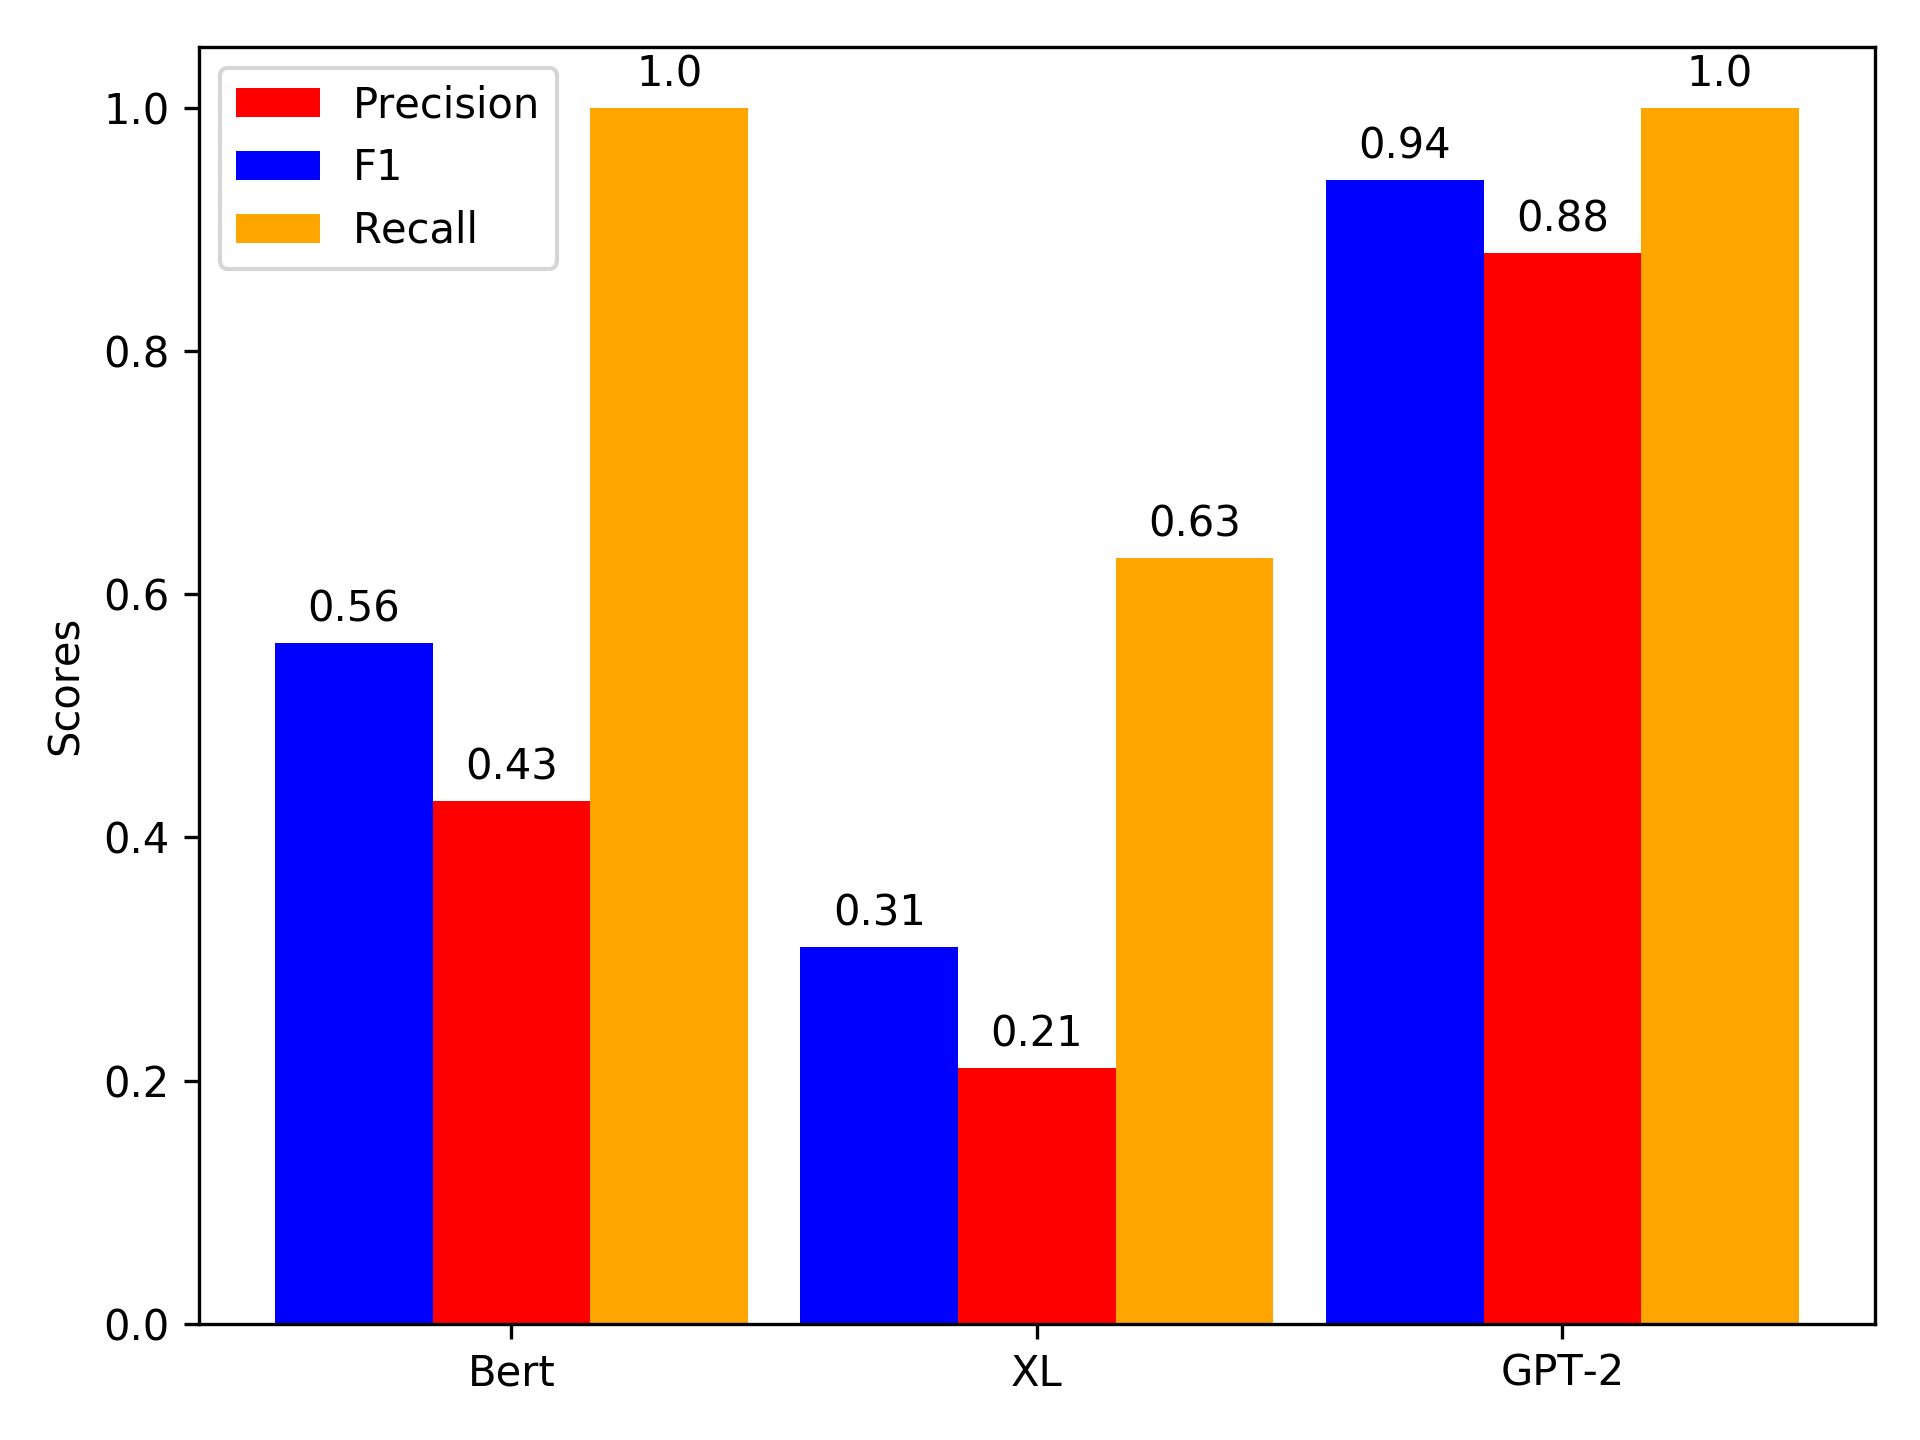
\includegraphics[trim={1cm 0.5cm 0cm 1cm}, width=0.322\textwidth]{results/average/regression_sequential_average_ratio_0.15.png}}\\
\caption{\label{fig:results_regression_sequential}Altering log sequences at different ratios, using regression, 5\% anomaly.}
\end{figure*}


\begin{figure*}[ht!]
   \subfloat[5\% alteration\label{fig:results_regression_qualitative_5}]{%
      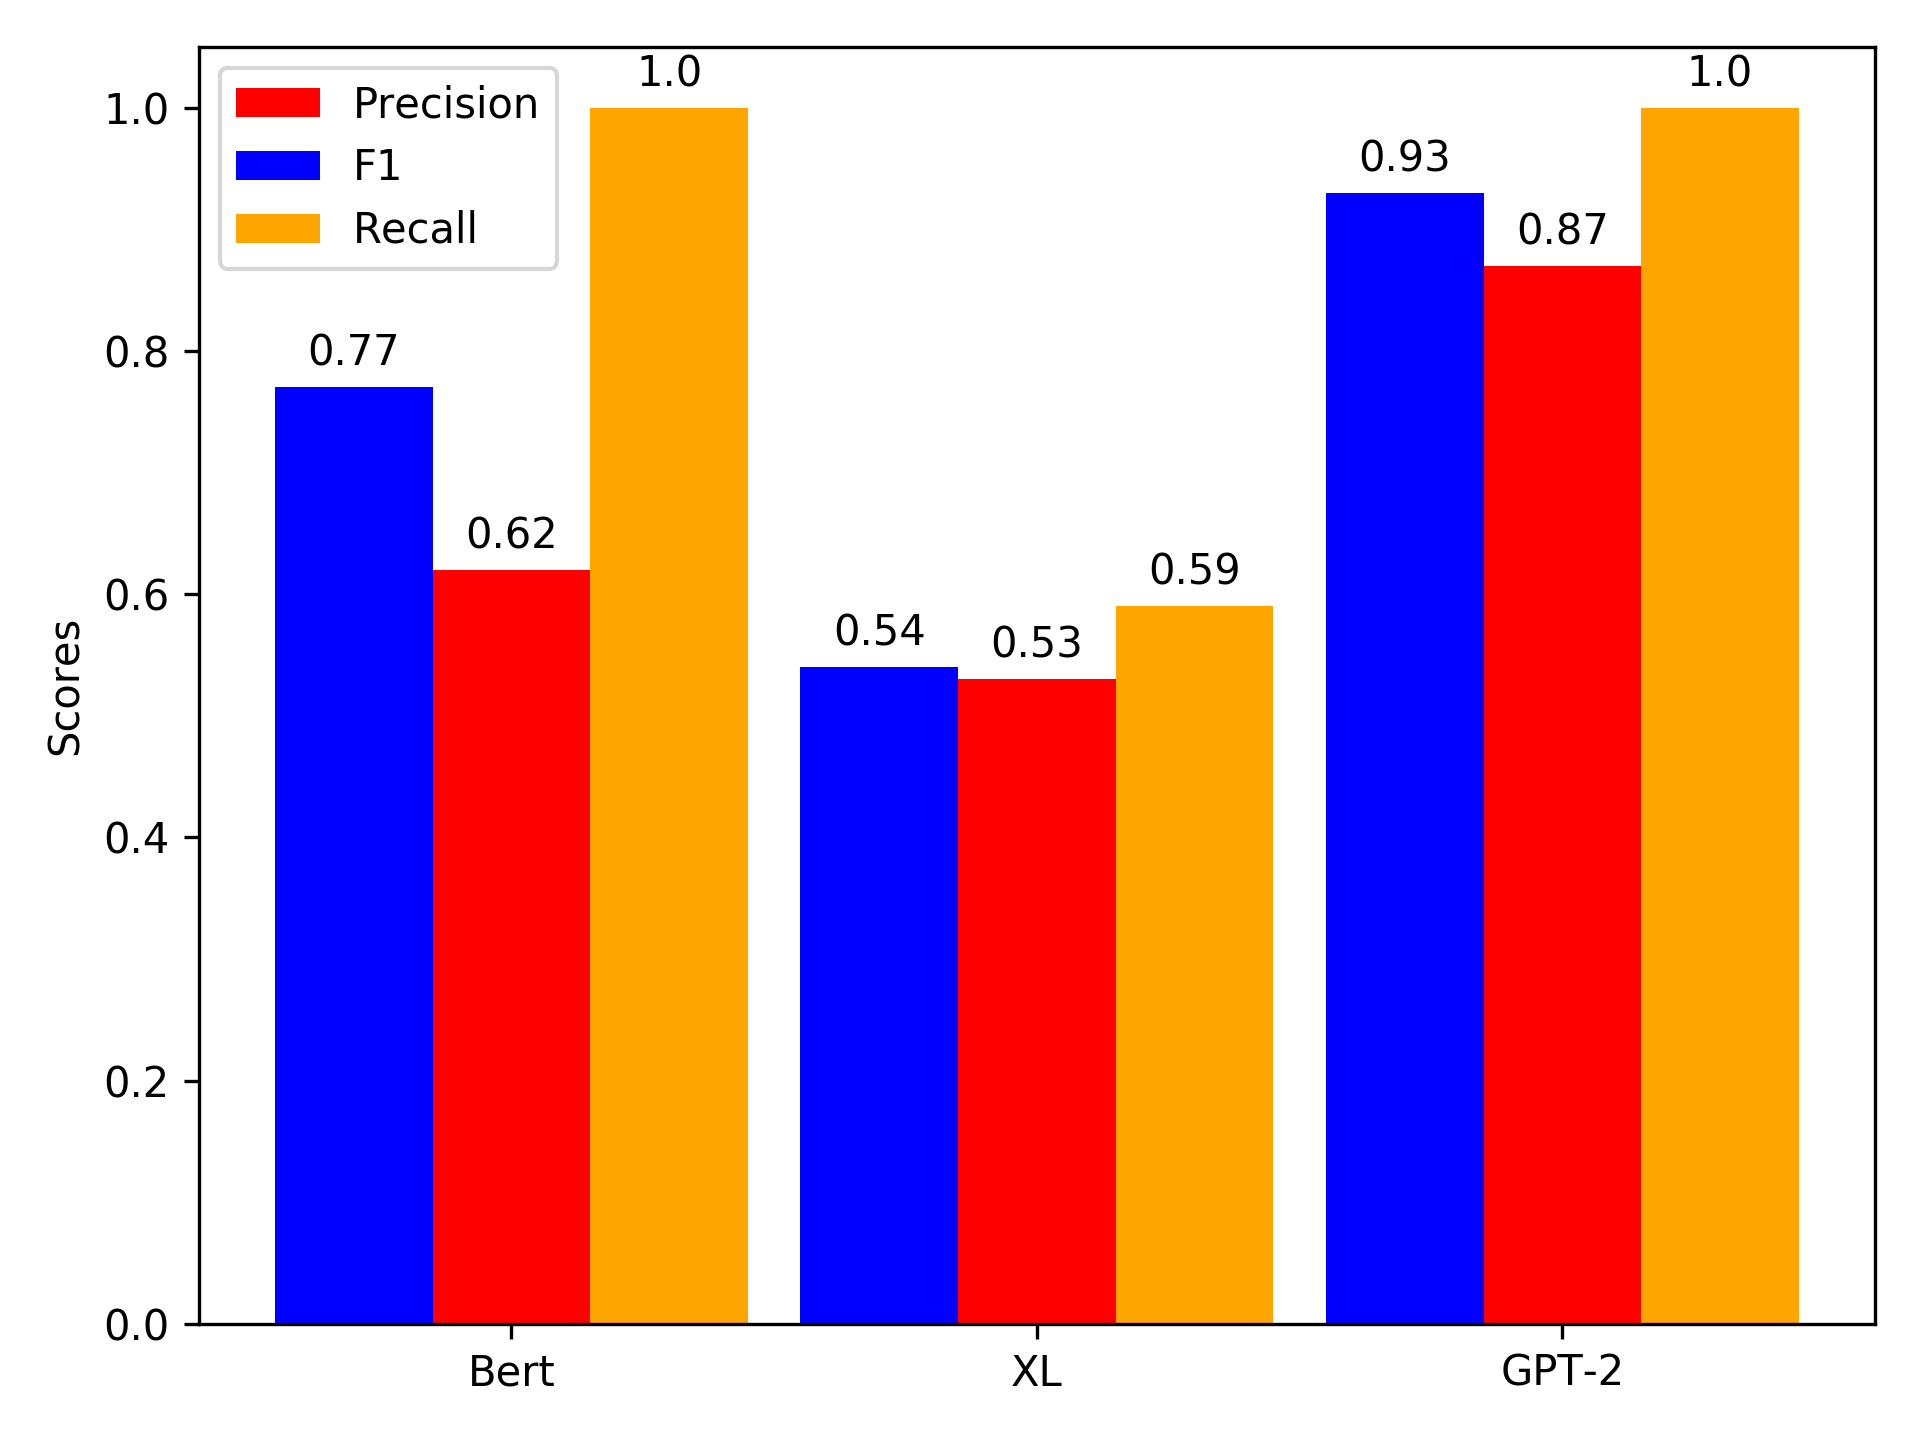
\includegraphics[trim={1cm 0.5cm 0cm 1cm}, width=0.322\textwidth]{results/average/regression_qualitative_average_ratio_0.05.png}}
\hspace{\fill}
   \subfloat[10\% alteration\label{fig:results_regression_qualitative_10} ]{%
      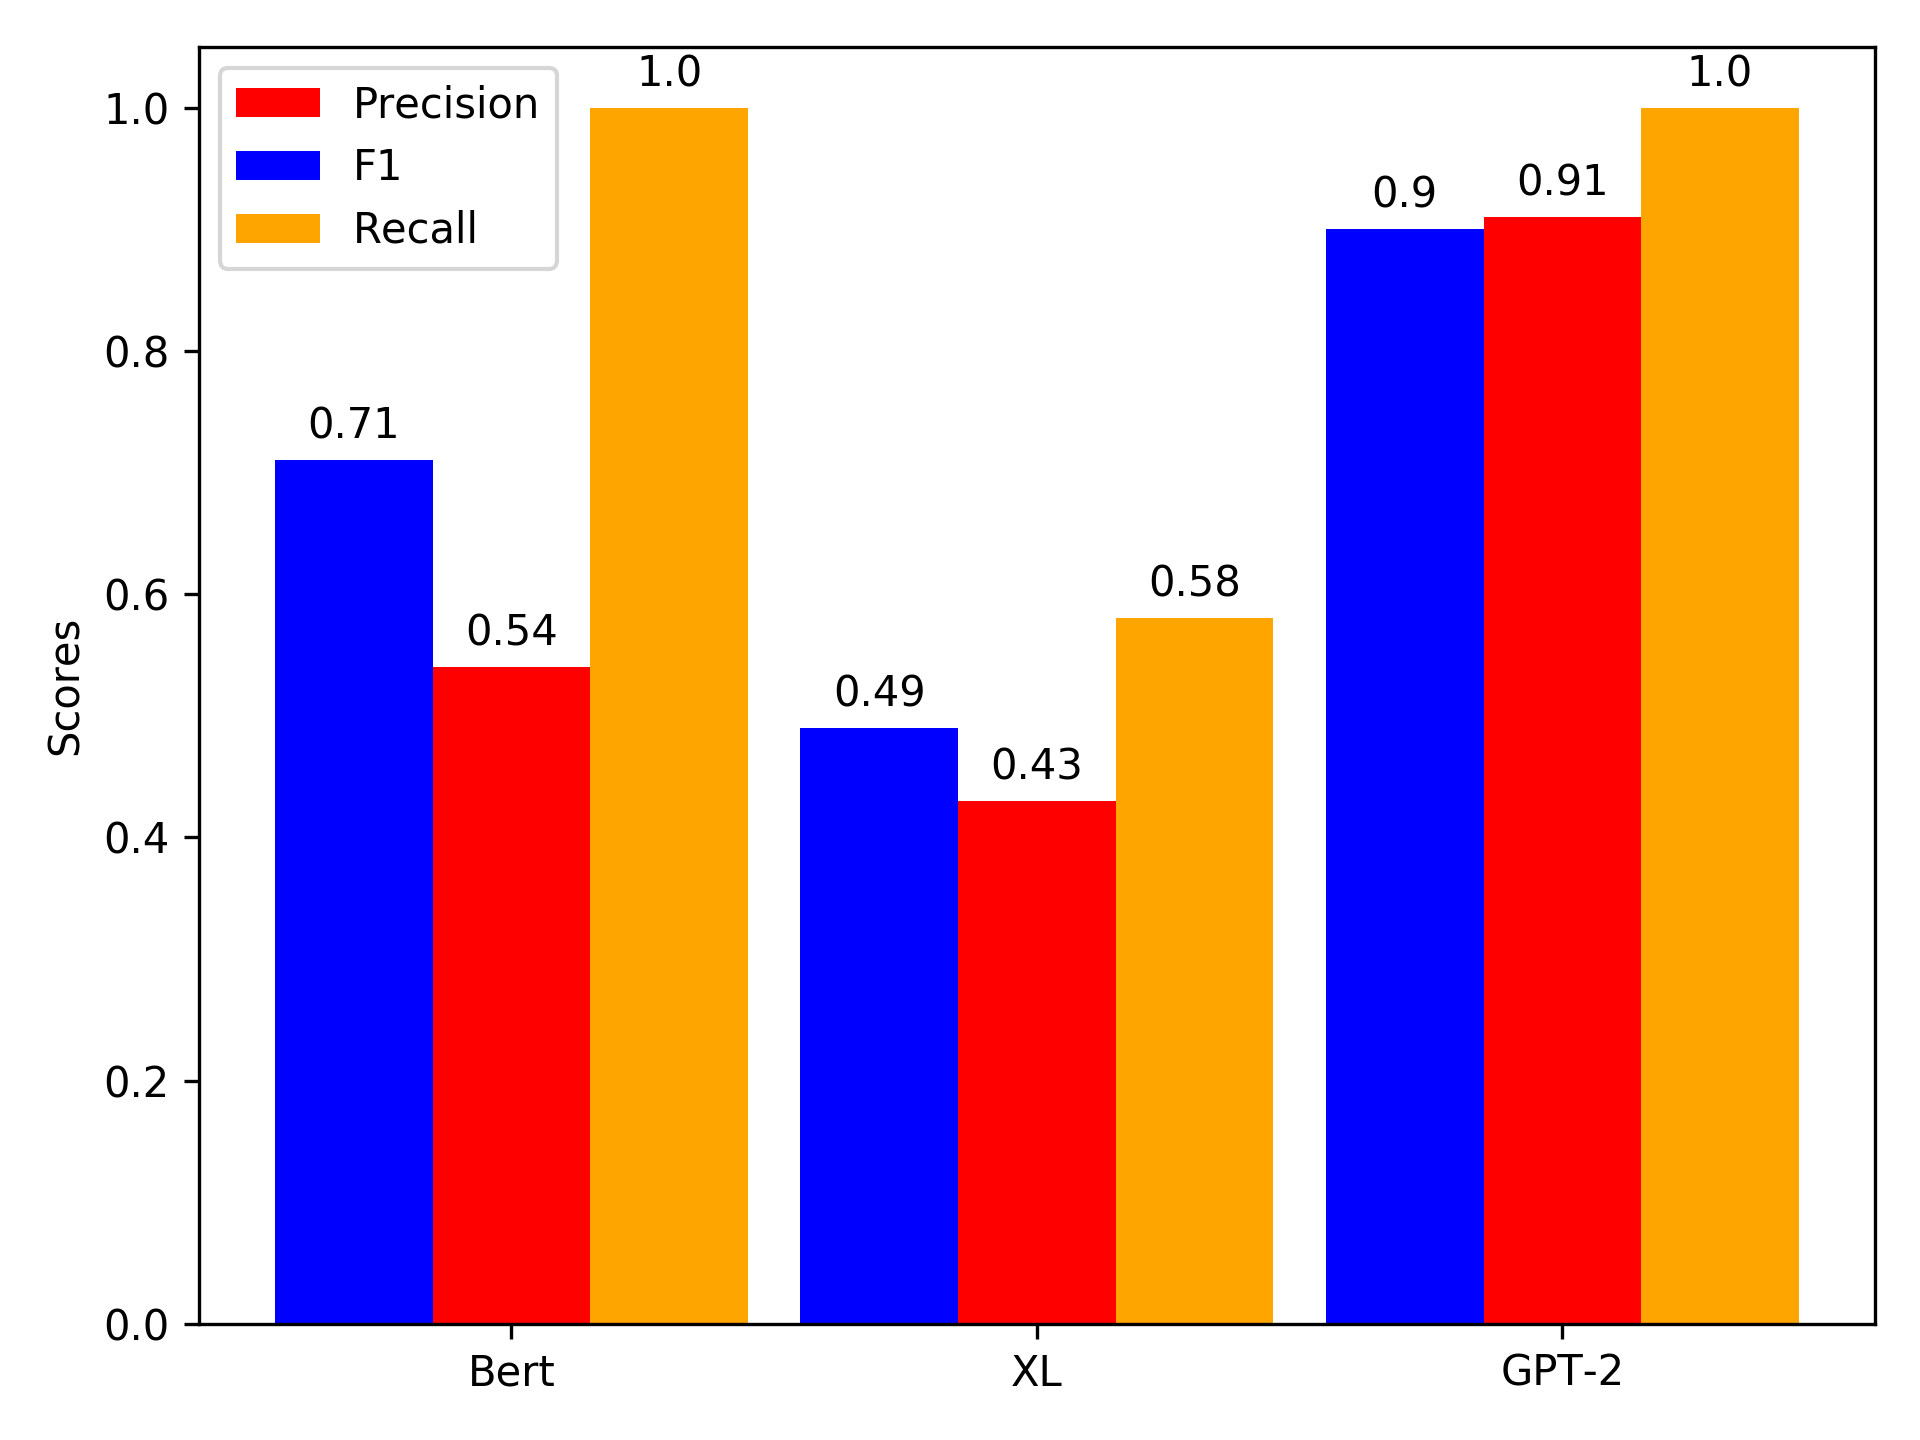
\includegraphics[trim={1cm 0.5cm 0cm 1cm}, width=0.322\textwidth]{results/average/regression_qualitative_average_ratio_0.10.png}}
\hspace{\fill}
   \subfloat[15\% alteration\label{fig:results_regression_qualitative_15}]{%
      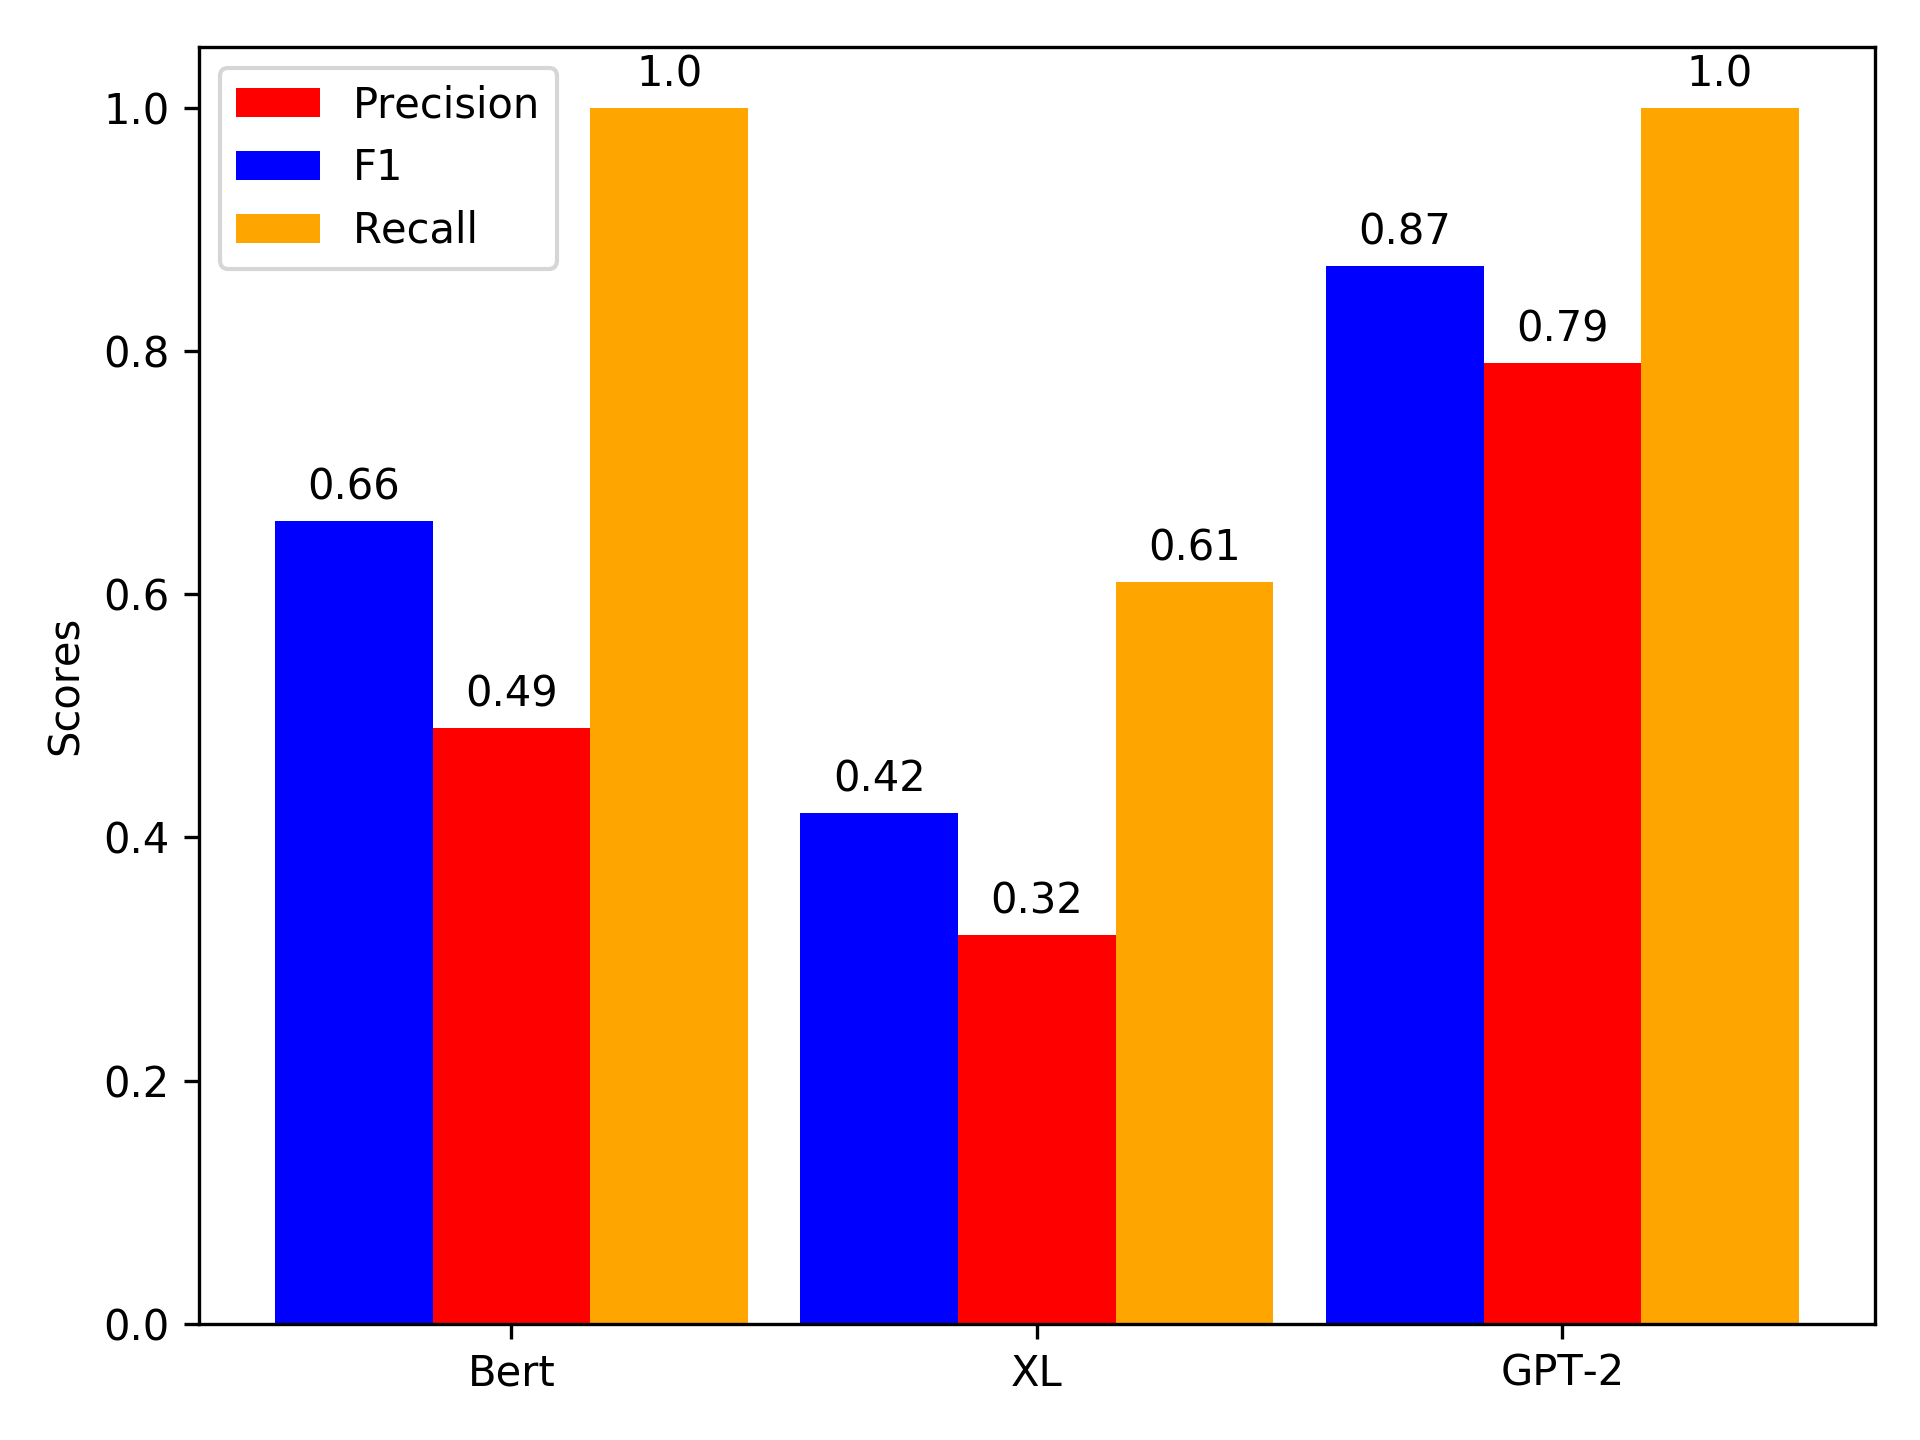
\includegraphics[trim={1cm 0.5cm 0cm 1cm}, width=0.322\textwidth]{results/average/regression_qualitative_average_ratio_0.15.png}}\\
\caption{\label{fig:results_regression_words}Altering log lines at different ratios, using regression, 5\% anomaly.}
\end{figure*}	

%%%%%



\begin{figure}[h]
  \centering
  \captionsetup{justification=centering}
  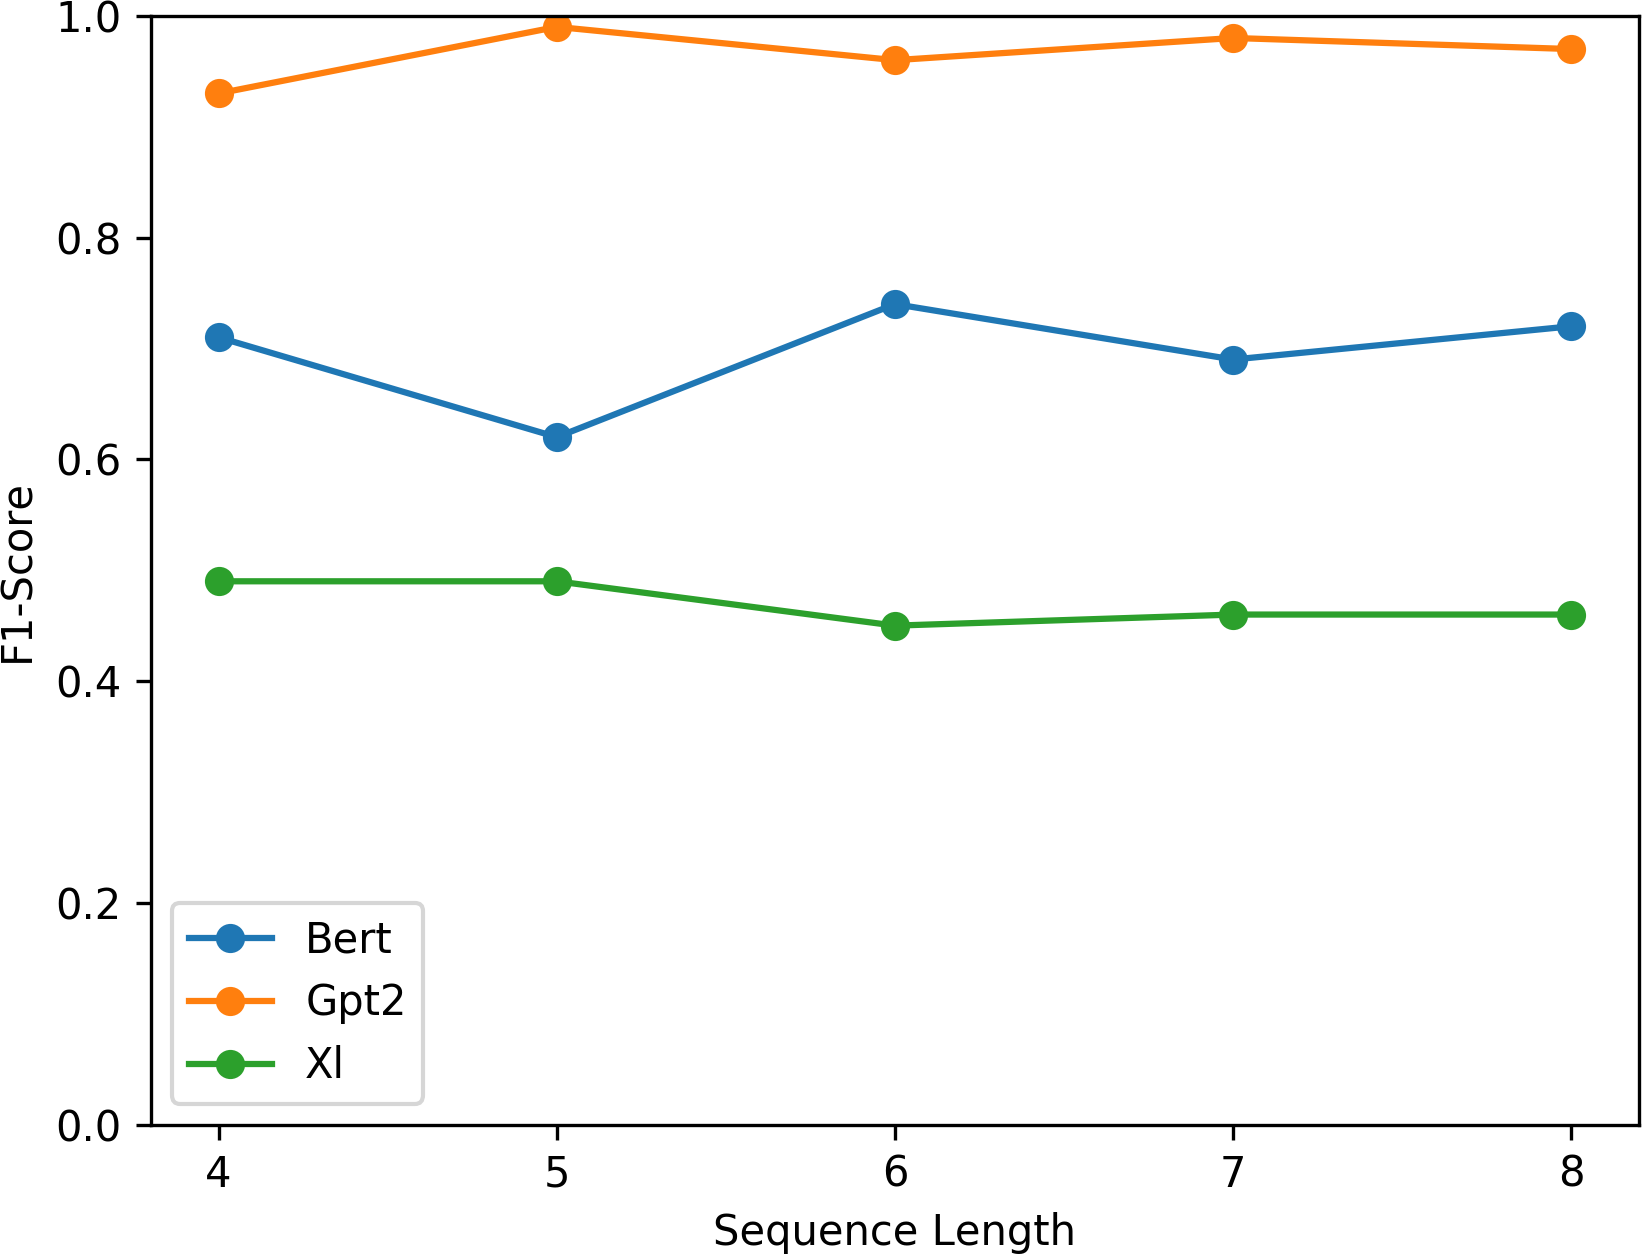
\includegraphics[width=9cm,height=6.5cm]{results/seq_len/sequence_len_regression.png}\\
  \caption{F1-Score for varying input sequence lengths, 15\% word insertion, 5\% anomaly, using regression.}
  \label{fig:seq_len_regression}
\end{figure}





%%%%%%%%%%%%%%%%
% CLASSIFICATION 
%%%%%%%%%%%%%%%%
\subsection{Classification \label{sec:results-classification}}
In this subsection, the results of the classification-based approach are presented, with the exact same boundary conditions as in \ref{sec:results-regression}. 
The ability of the system to detect injected anomalies, despite injected alterations on the sequences of logs, can be seen in \ref{fig:results_multiclass_sequential}. 
The impact of alterations on the sequence of logs, i.e. deleting, shuffling and duplicating events are summarised in figure \ref{fig:results_regression_sequential}. Again, only average results on the individual injections are presented. Results broken down by each alteration can be found in the appendix \ref{appendix:classification}. 

In contrary to the results using regression, the classification approach seems most fit for Bert and much less for GPT-2. This is probably due to the smaller cosine distance between the templates in GPT-2, which makes it harder for the system to correctly assign the templates to the classes in the prediction process. Yet, for the reverse order injection, which can be seen in figure \ref{fig:multiclass_reverse_order}, the results are better for GPT-2, than with the regression approach.

Additionally to the alterations on the log sequences, the results alterations on the log events themselves, i.e. inserting, removing and replacing words are of interest. The results of this experiment can be seen in figure \ref{fig:results_multiclass_sequential}. Again, the alterations are not injected all at once, but independently - the figure shows averaged results.

The impact of the input sequence length can be seen in \ref{fig:seq_len_regression}. Bert again seems to profit slightly from sequence lengths longer than 6 or 7, whereas the quality of results for XL-Transformers and GPT-2 seem to have a tendency to degrade in prediction quality for longer input sequence lengths.


\begin{figure}[h]
  \centering
  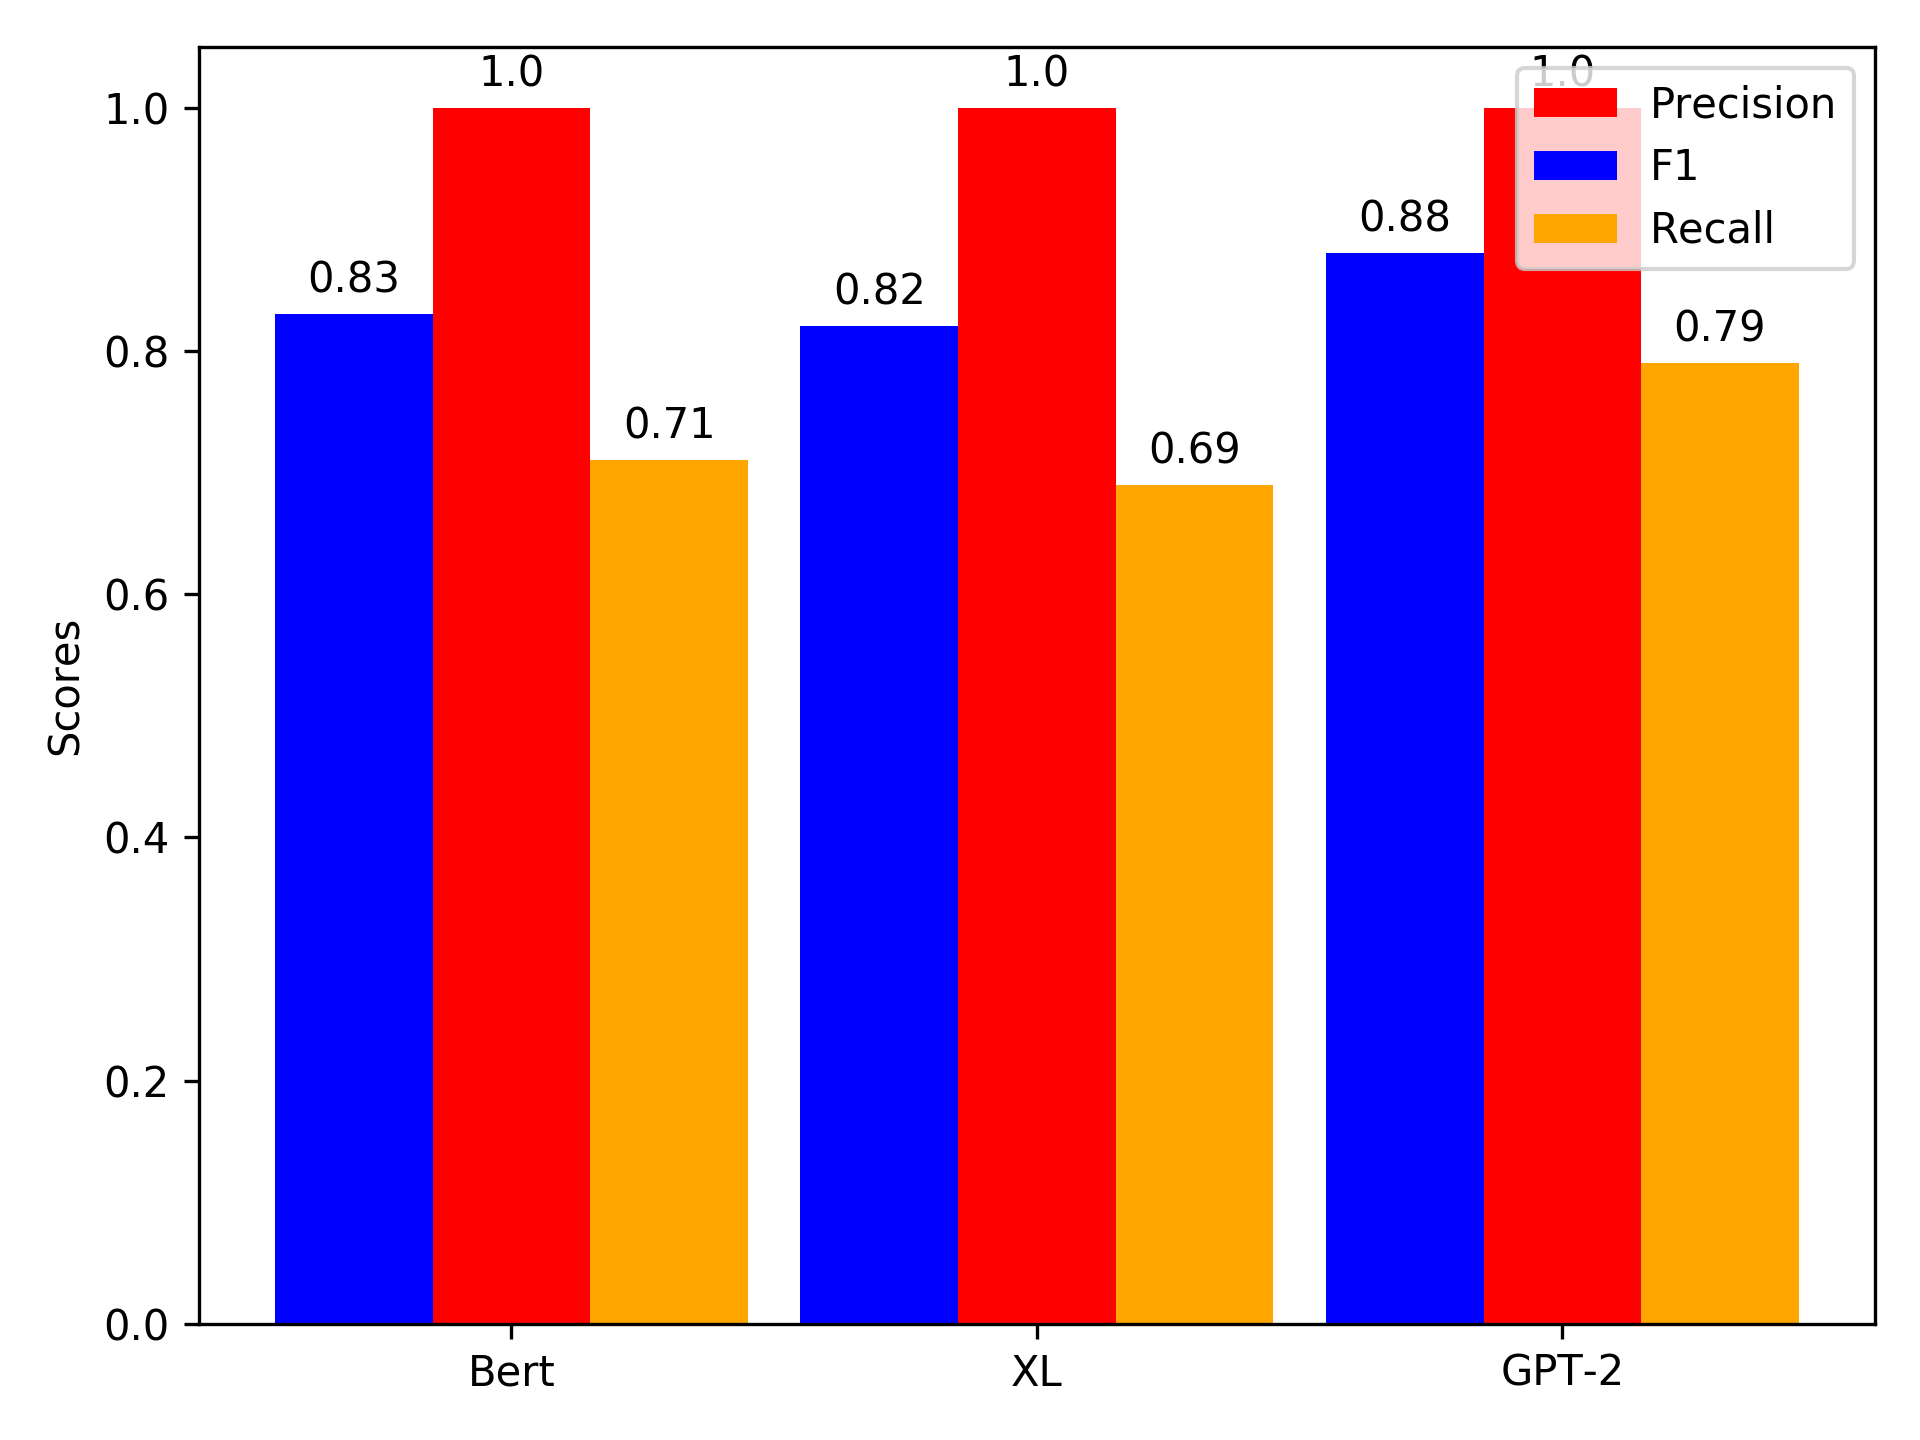
\includegraphics[width=6cm,height=4.5cm]{results/classification_sequence/multiclass_reverse.png}\\
  \caption{Scores for detecting reversed order of log events, using classification.}
  \label{fig:multiclass_reverse_order}
\end{figure}
% multiclass sequential
\begin{figure*}[ht!]
   \subfloat[5\% alteration\label{fig:results_multiclass_sequential_5}]{%
      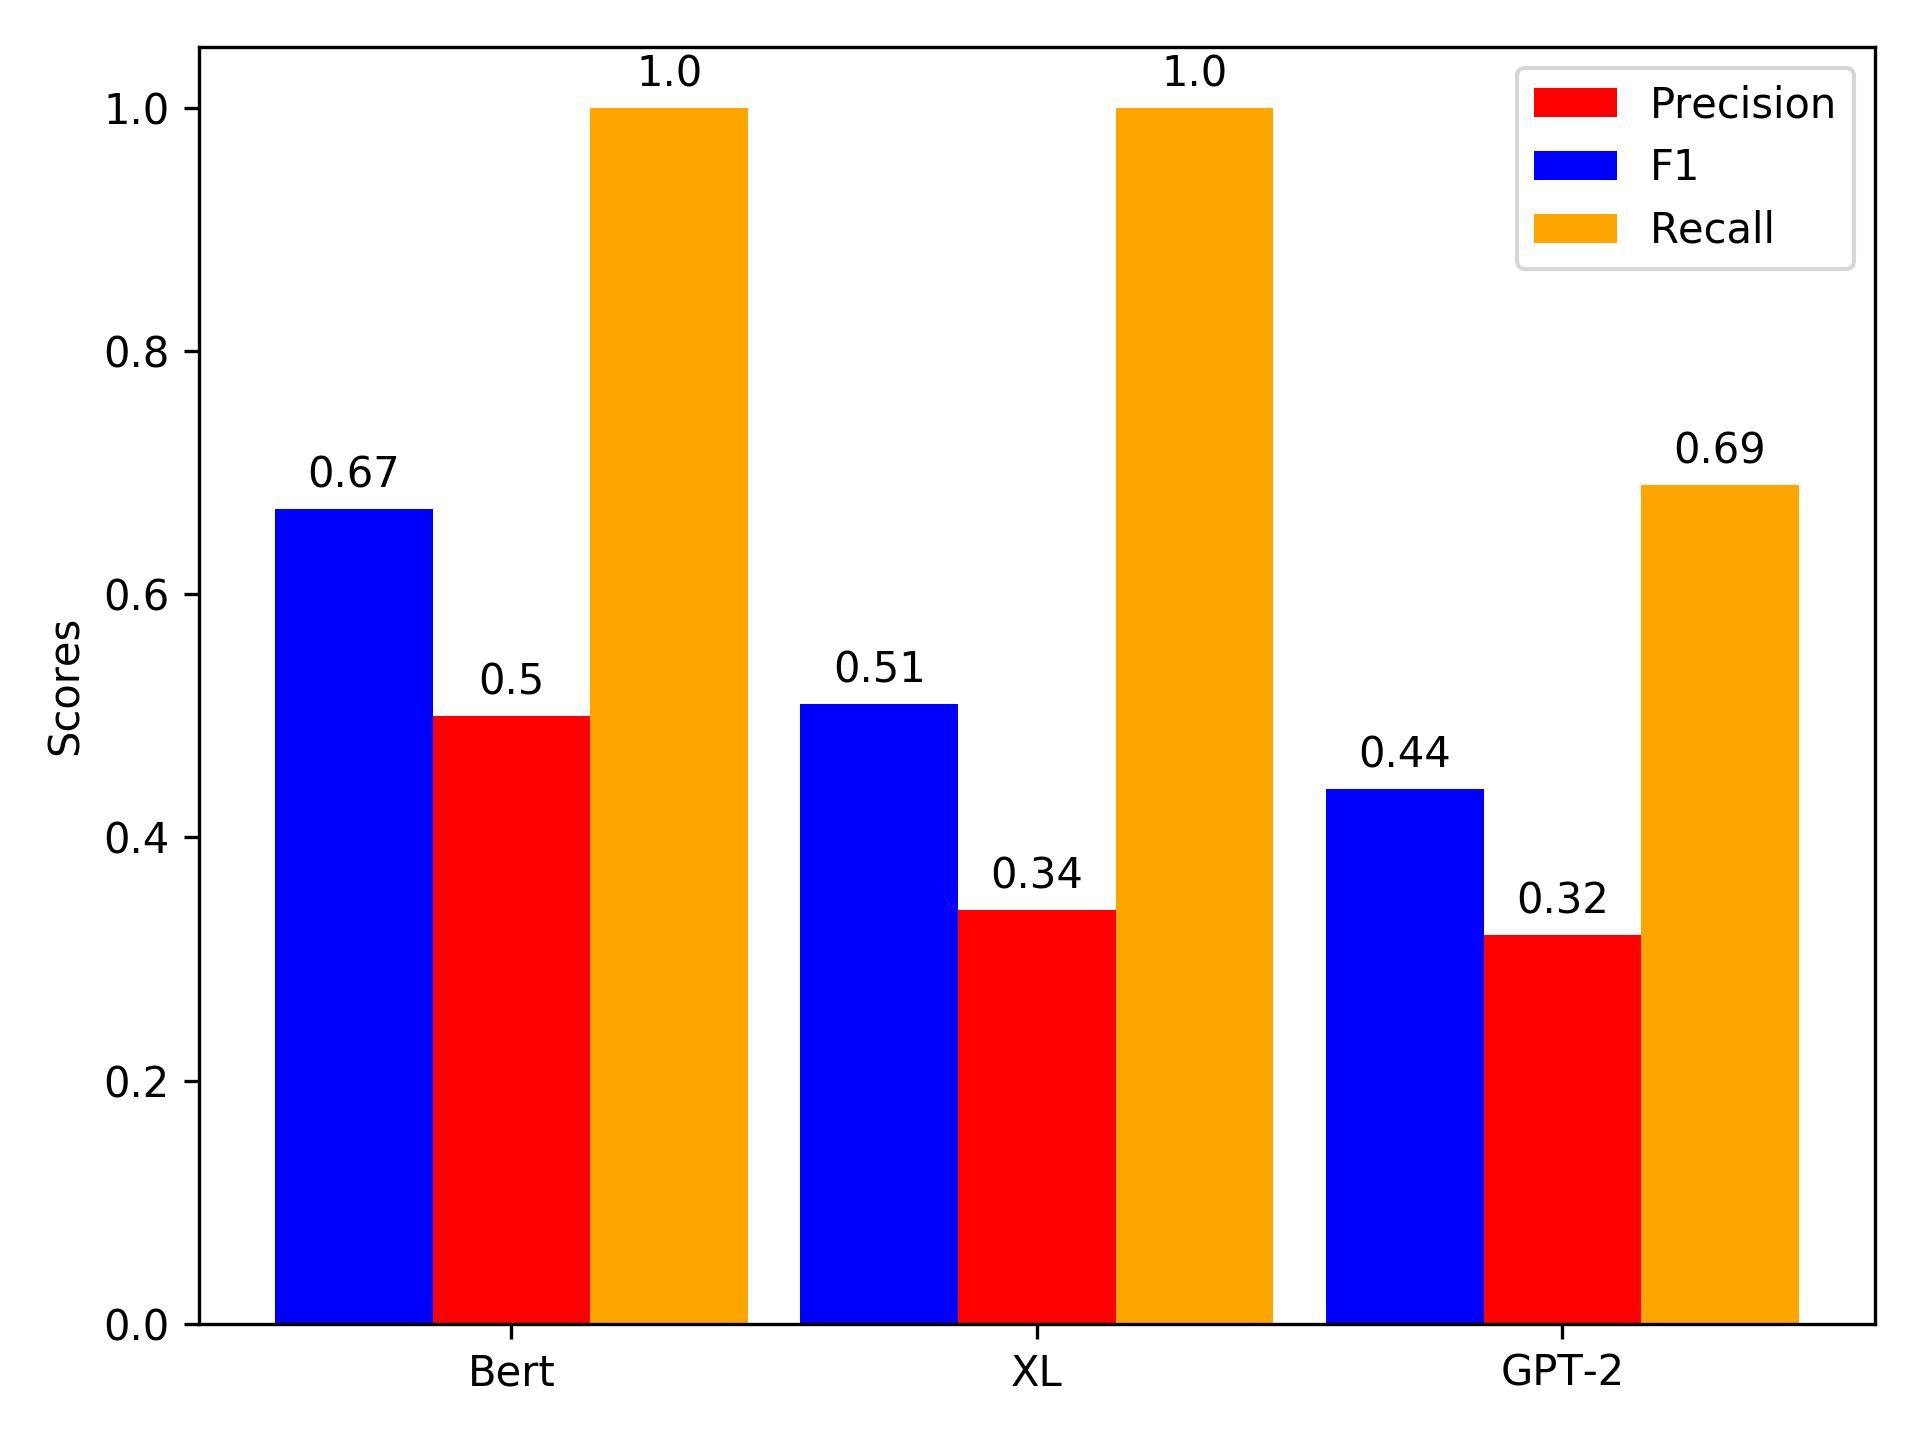
\includegraphics[trim={1cm 0.5cm 0cm 1cm}, width=0.322\textwidth]{results/average/multiclass_sequential_average_ratio_0.05.png}}
\hspace{\fill}
   \subfloat[10\% alteration\label{fig:results_multiclass_sequential_10} ]{%
      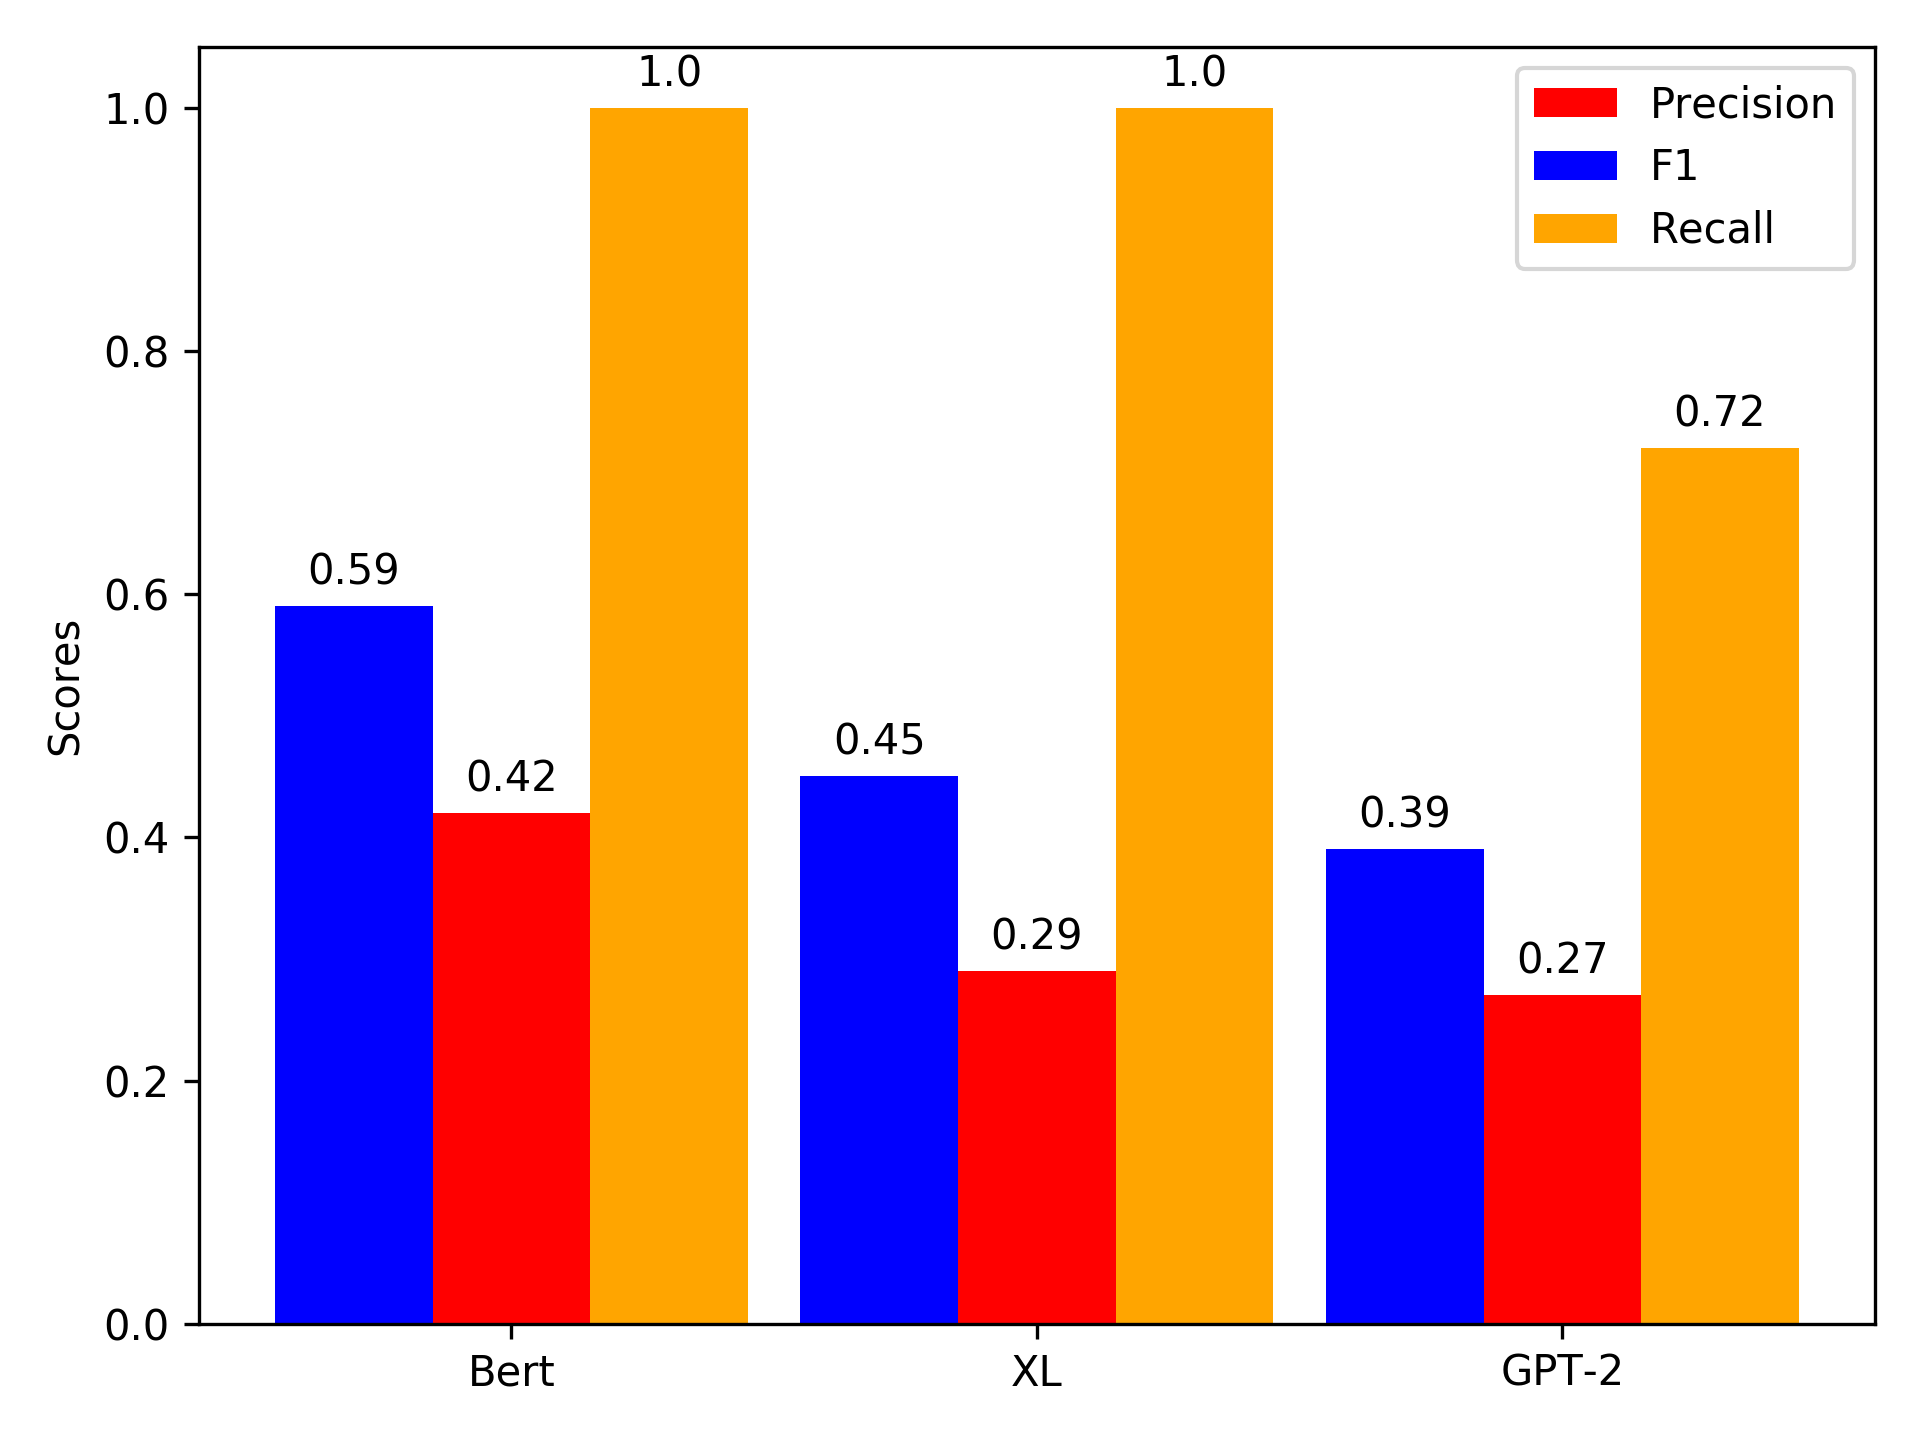
\includegraphics[trim={1cm 0.5cm 0cm 1cm}, width=0.322\textwidth]{results/average/multiclass_sequential_average_ratio_0.10.png}}
\hspace{\fill}
   \subfloat[15\% alteration\label{fig:results_multiclass_sequential_15}]{%
      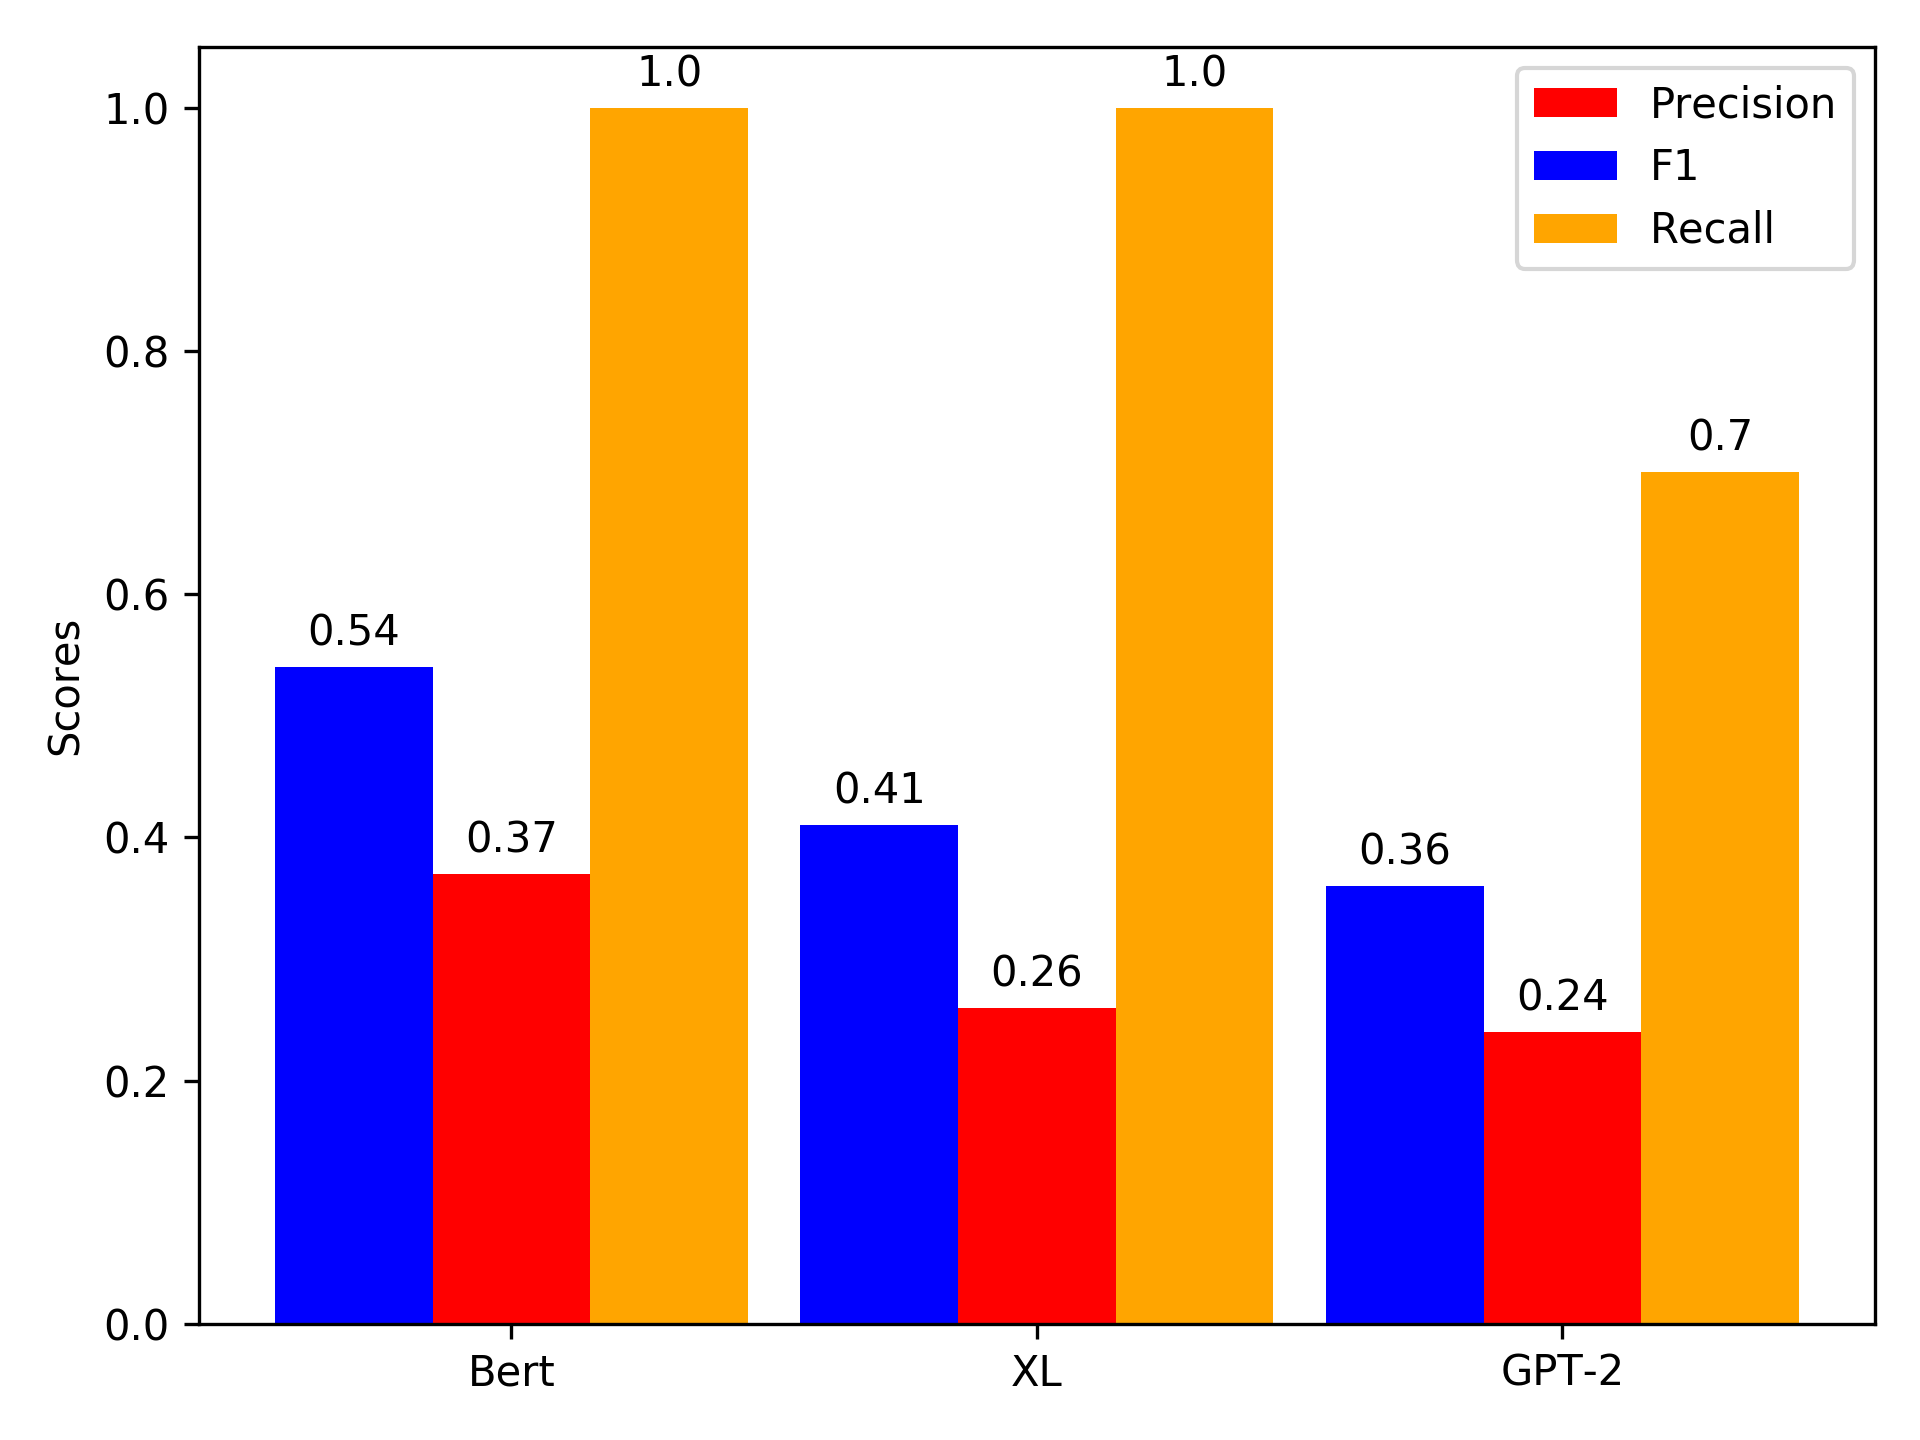
\includegraphics[trim={1cm 0.5cm 0cm 1cm}, width=0.322\textwidth]{results/average/multiclass_sequential_average_ratio_0.15.png}}\\
\caption{\label{fig:results_multiclass_sequential}Altering log lines at different ratios, using classification, 5\% anomaly.}
\end{figure*}

%multiclass qualitative
\begin{figure*}[ht!]
   \subfloat[5\% alteration\label{fig:results_multiclass_qualitative_5}]{%
      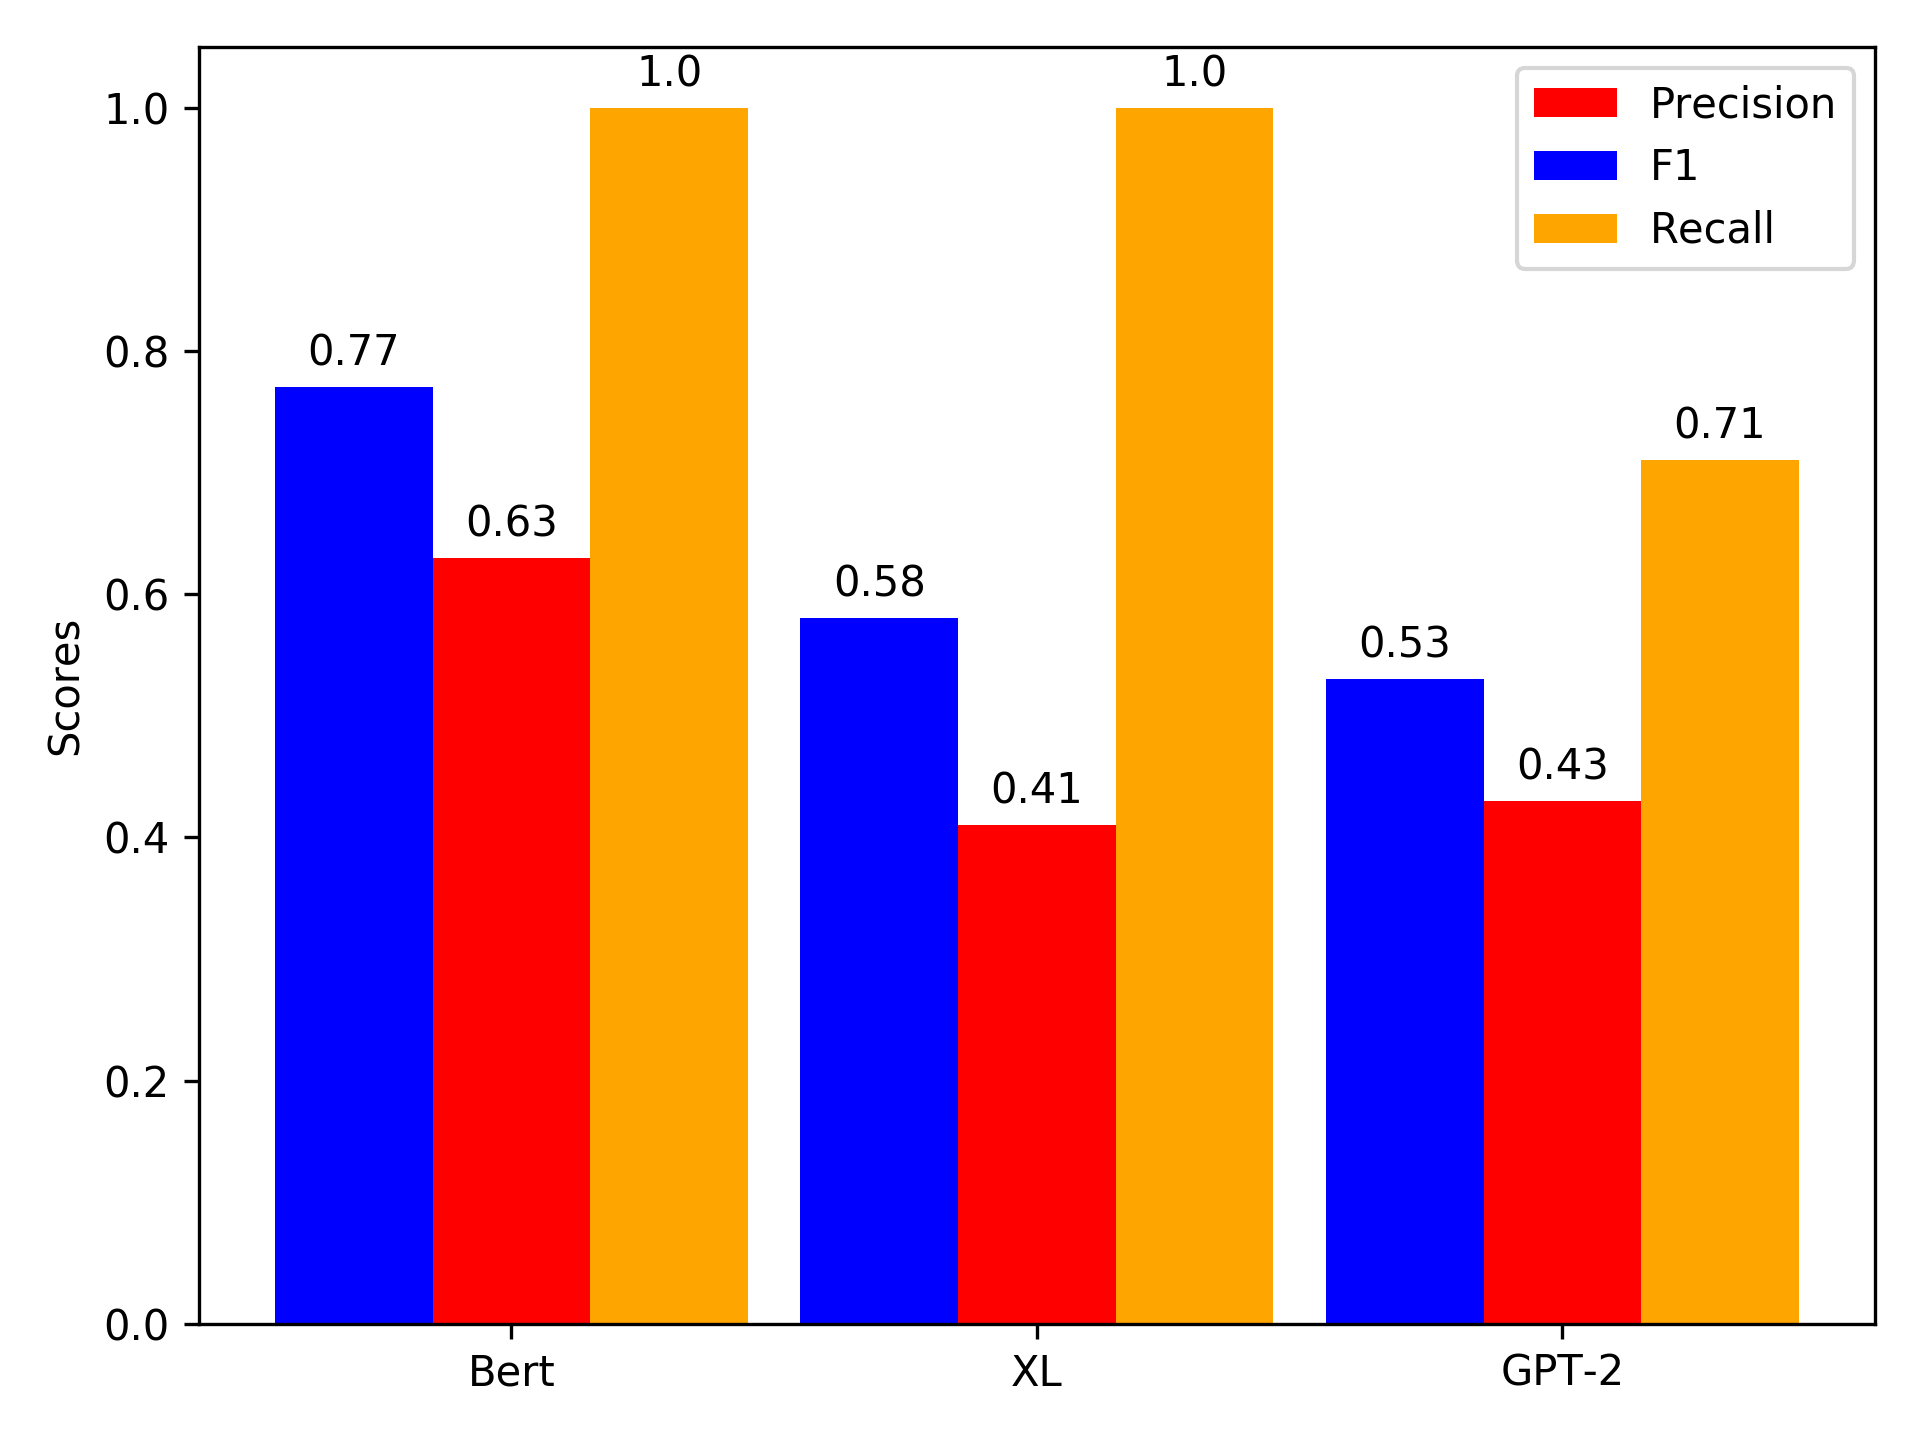
\includegraphics[trim={1cm 0.5cm 0cm 1cm}, width=0.322\textwidth]{results/average/multiclass_qualitative_average_ratio_0.05.png}}
\hspace{\fill}
   \subfloat[10\% alteration\label{fig:results_multiclass_qualitative_10} ]{%
      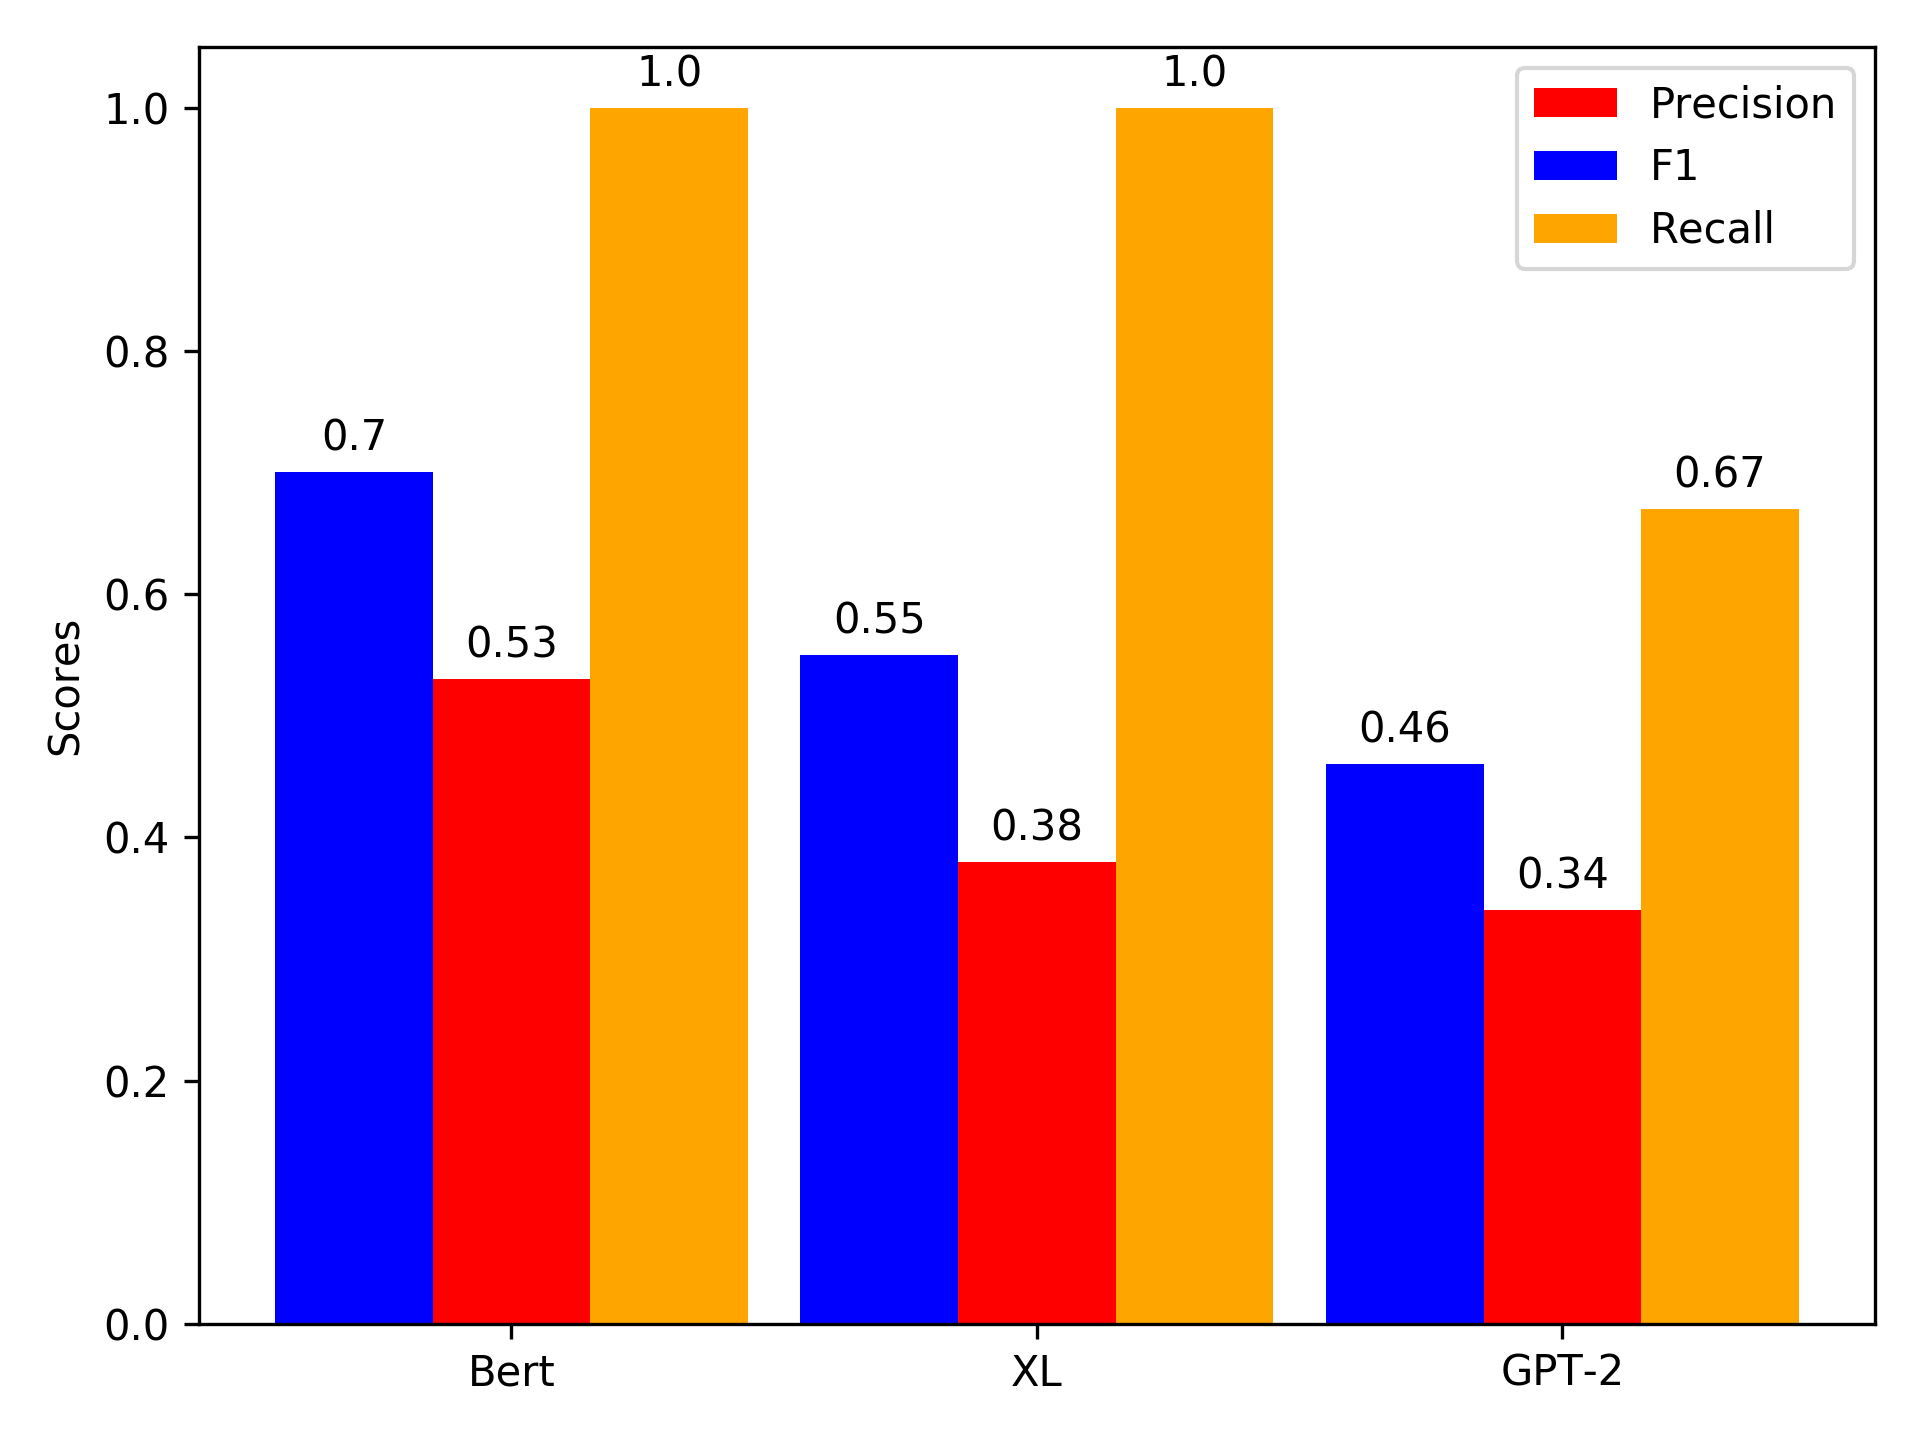
\includegraphics[trim={1cm 0.5cm 0cm 1cm}, width=0.322\textwidth]{results/average/multiclass_qualitative_average_ratio_0.10.png}}
\hspace{\fill}
   \subfloat[15\% alteration\label{fig:results_multiclass_qualitative_15}]{%
      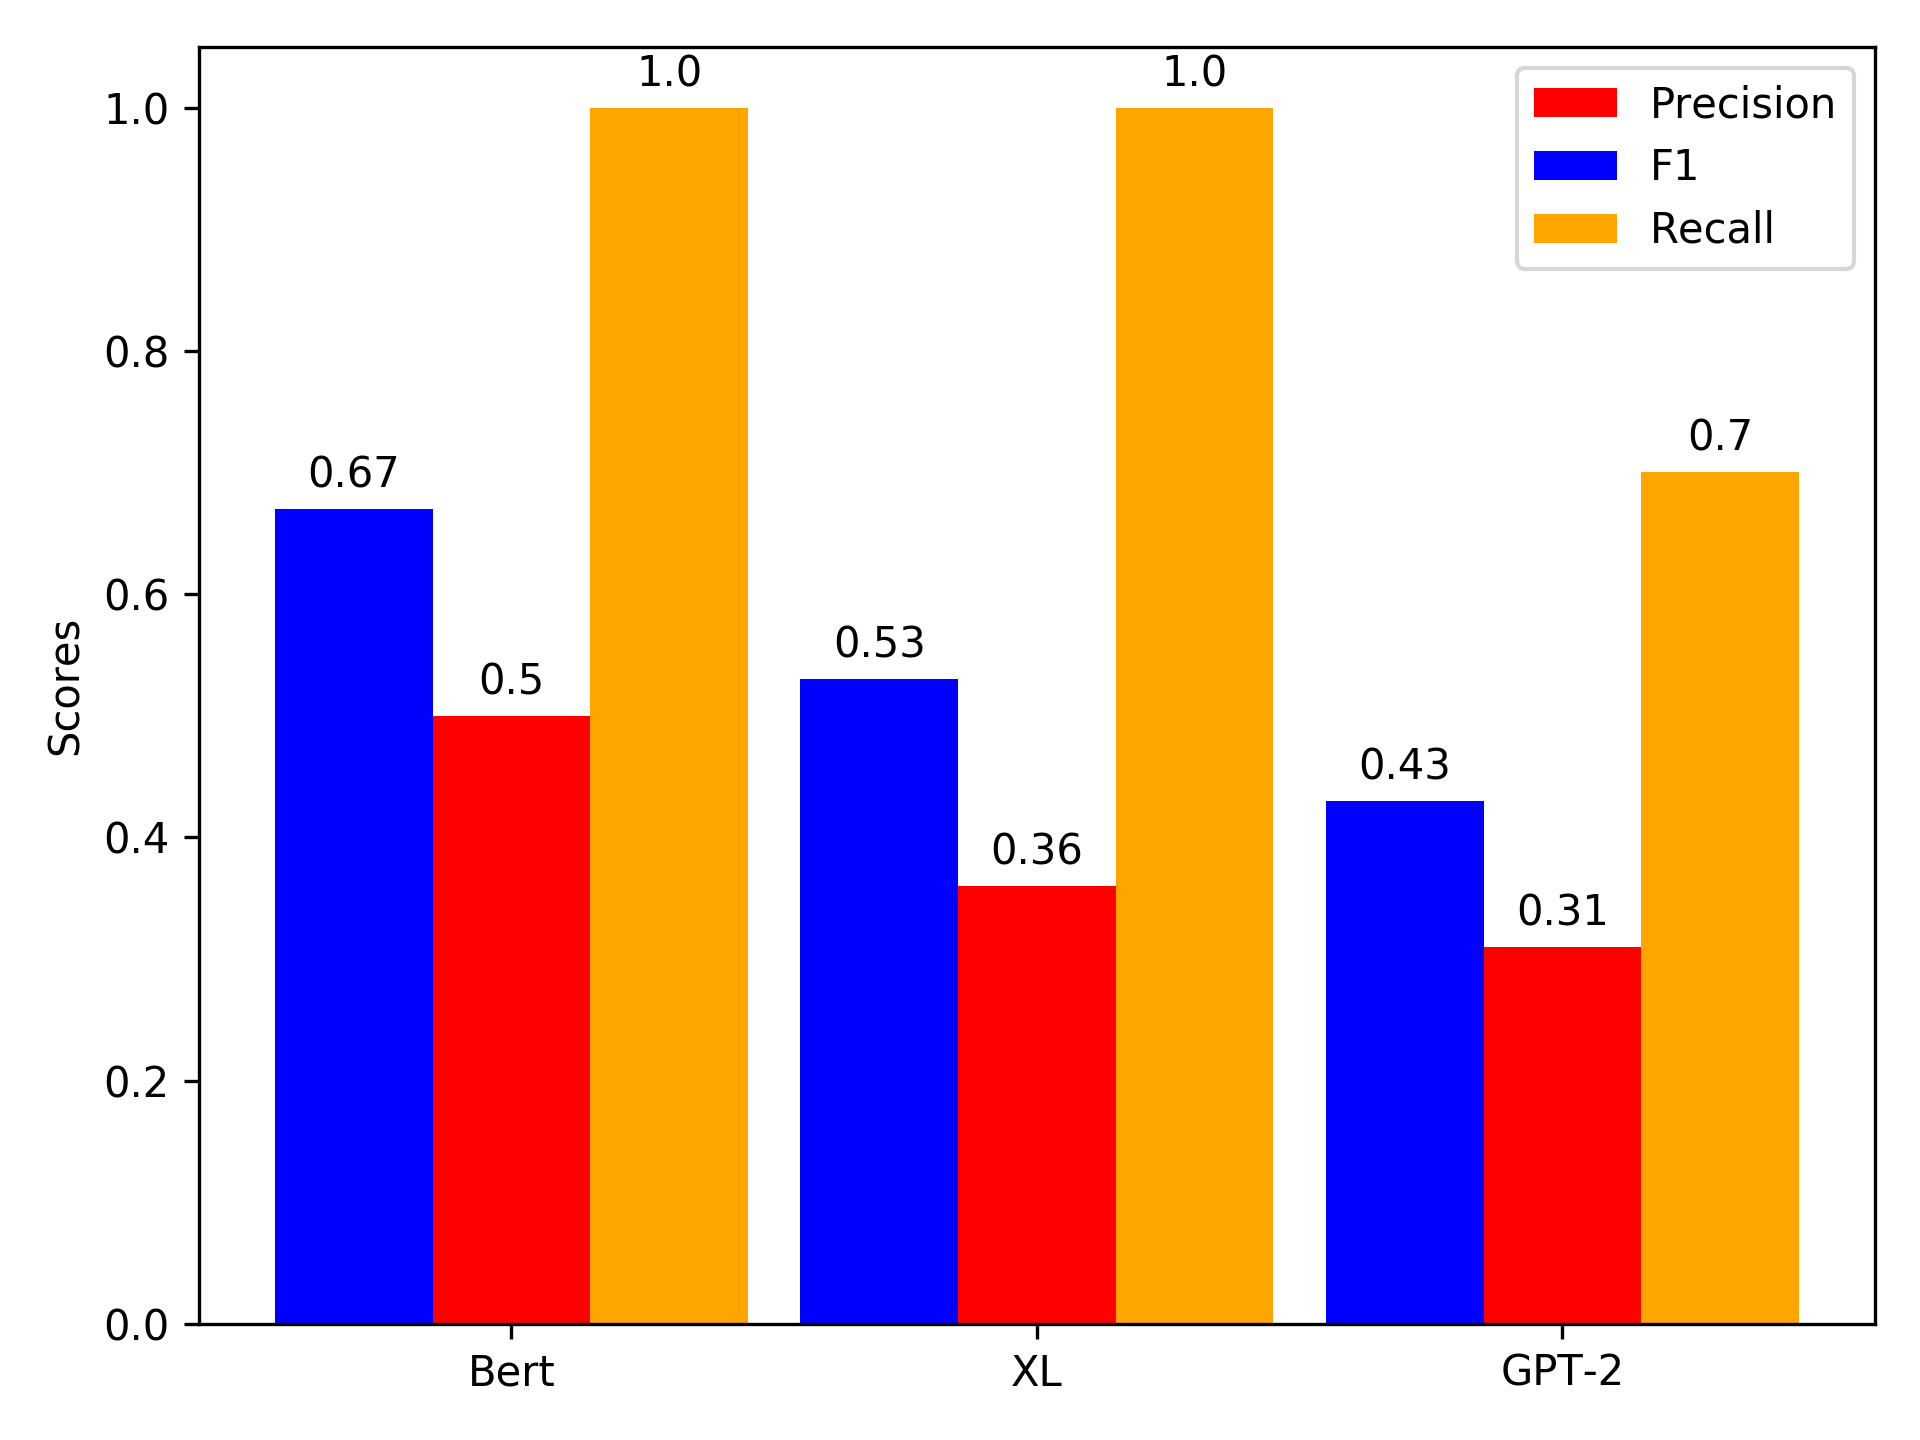
\includegraphics[trim={1cm 0.5cm 0cm 1cm}, width=0.322\textwidth]{results/average/multiclass_qualitative_average_ratio_0.15.png}}\\
\caption{\label{fig:results_multiclass_qualitative}Altering log events at different ratios, using classification, 5\% anomaly.}
\end{figure*}

% multiclass sequence length
\begin{figure}[h]
  \centering
  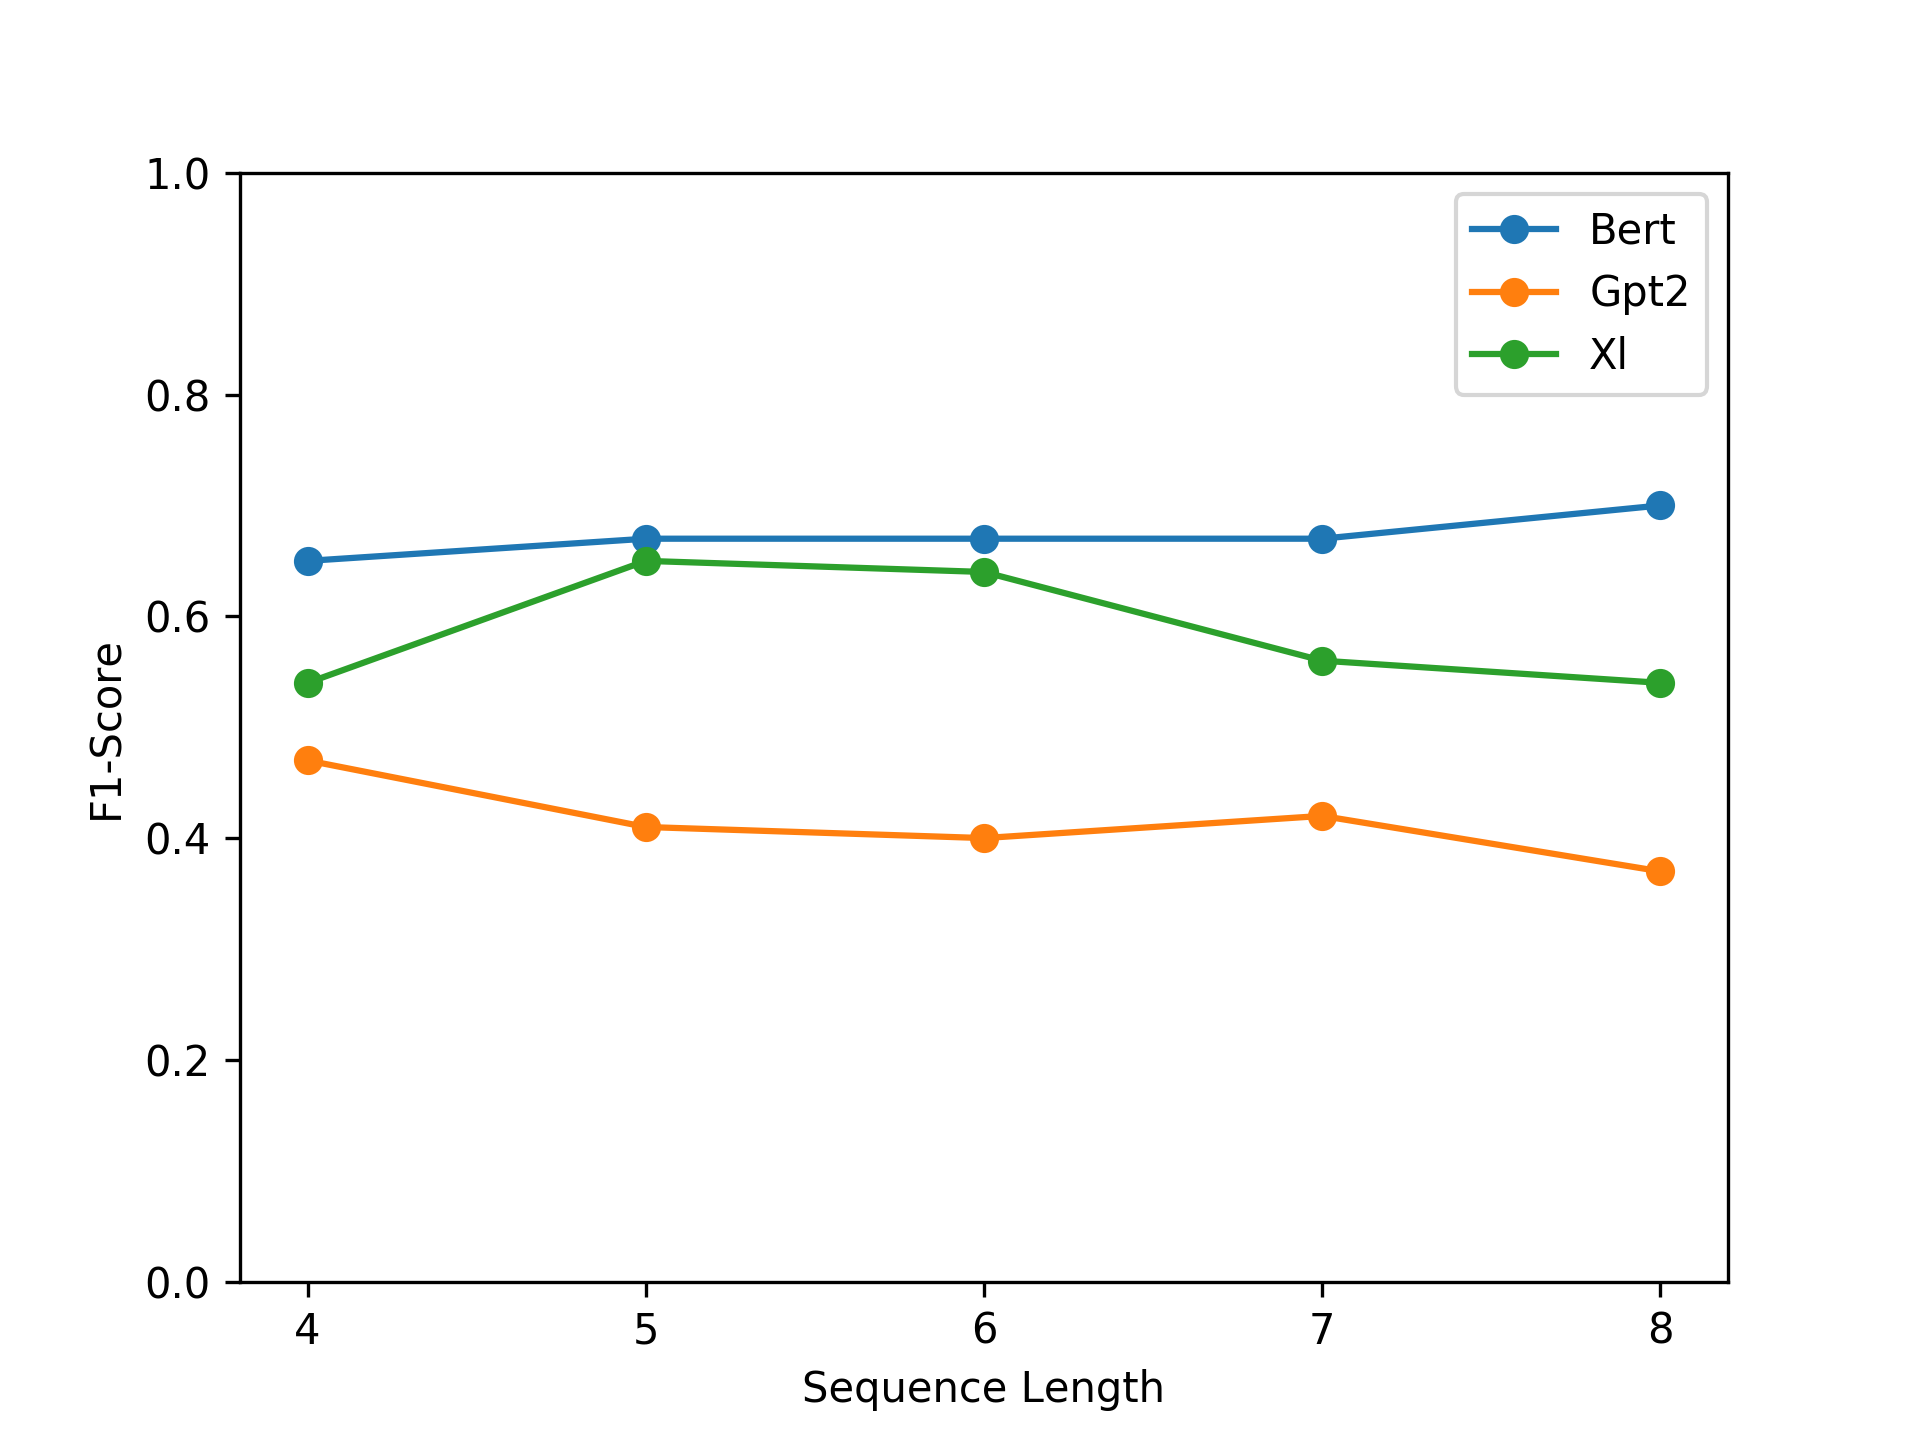
\includegraphics[width=9cm,height=6.5cm]{results/seq_len/sequence_len_classification.png}\\
  \caption{F1-Score for different input sequence lengths, with 15\% word insertion, using classification.}
  \label{fig:seq_len_classification}
\end{figure}


%%%%%
%%%%%
%%%%%

%%%%%%% TRANSFER LEARNING
\subsection{Transfer Learning\label{sec:results_transfer}}
In this subsection, the results of the transfer learning experiment are presented, using the classification-based approach in \ref{sec:results-classification-transfer} and the regression-based approach in \ref{sec:results-regression-transfer}.


\subsubsection{Transfer learning using the regression-based approach \label{sec:results-regression-transfer}}

As described in \ref{sec:transfer_learning_setup}, the alterations that were injected separately in the experiments on one dataset in the last section, are now injected all at once, to simulate a different dataset. Figure \ref{fig:results_transfer_regression} shows the results for alterations on 5\%, 10\% and 15\% of the log lines of all possible alterations at the same time, after 60 epochs of training on dataset A and 5 epochs of training on dataset B. It is clearly visible, that Bert and XL-Transformers are both degrading substantially in all metrics, yet GPT-2 achieves good results even with an increased alteration ratio.

\begin{figure*}[ht!]
   \subfloat[5\% alteration\label{fig:results_transfer_regression_0.05}]{%
      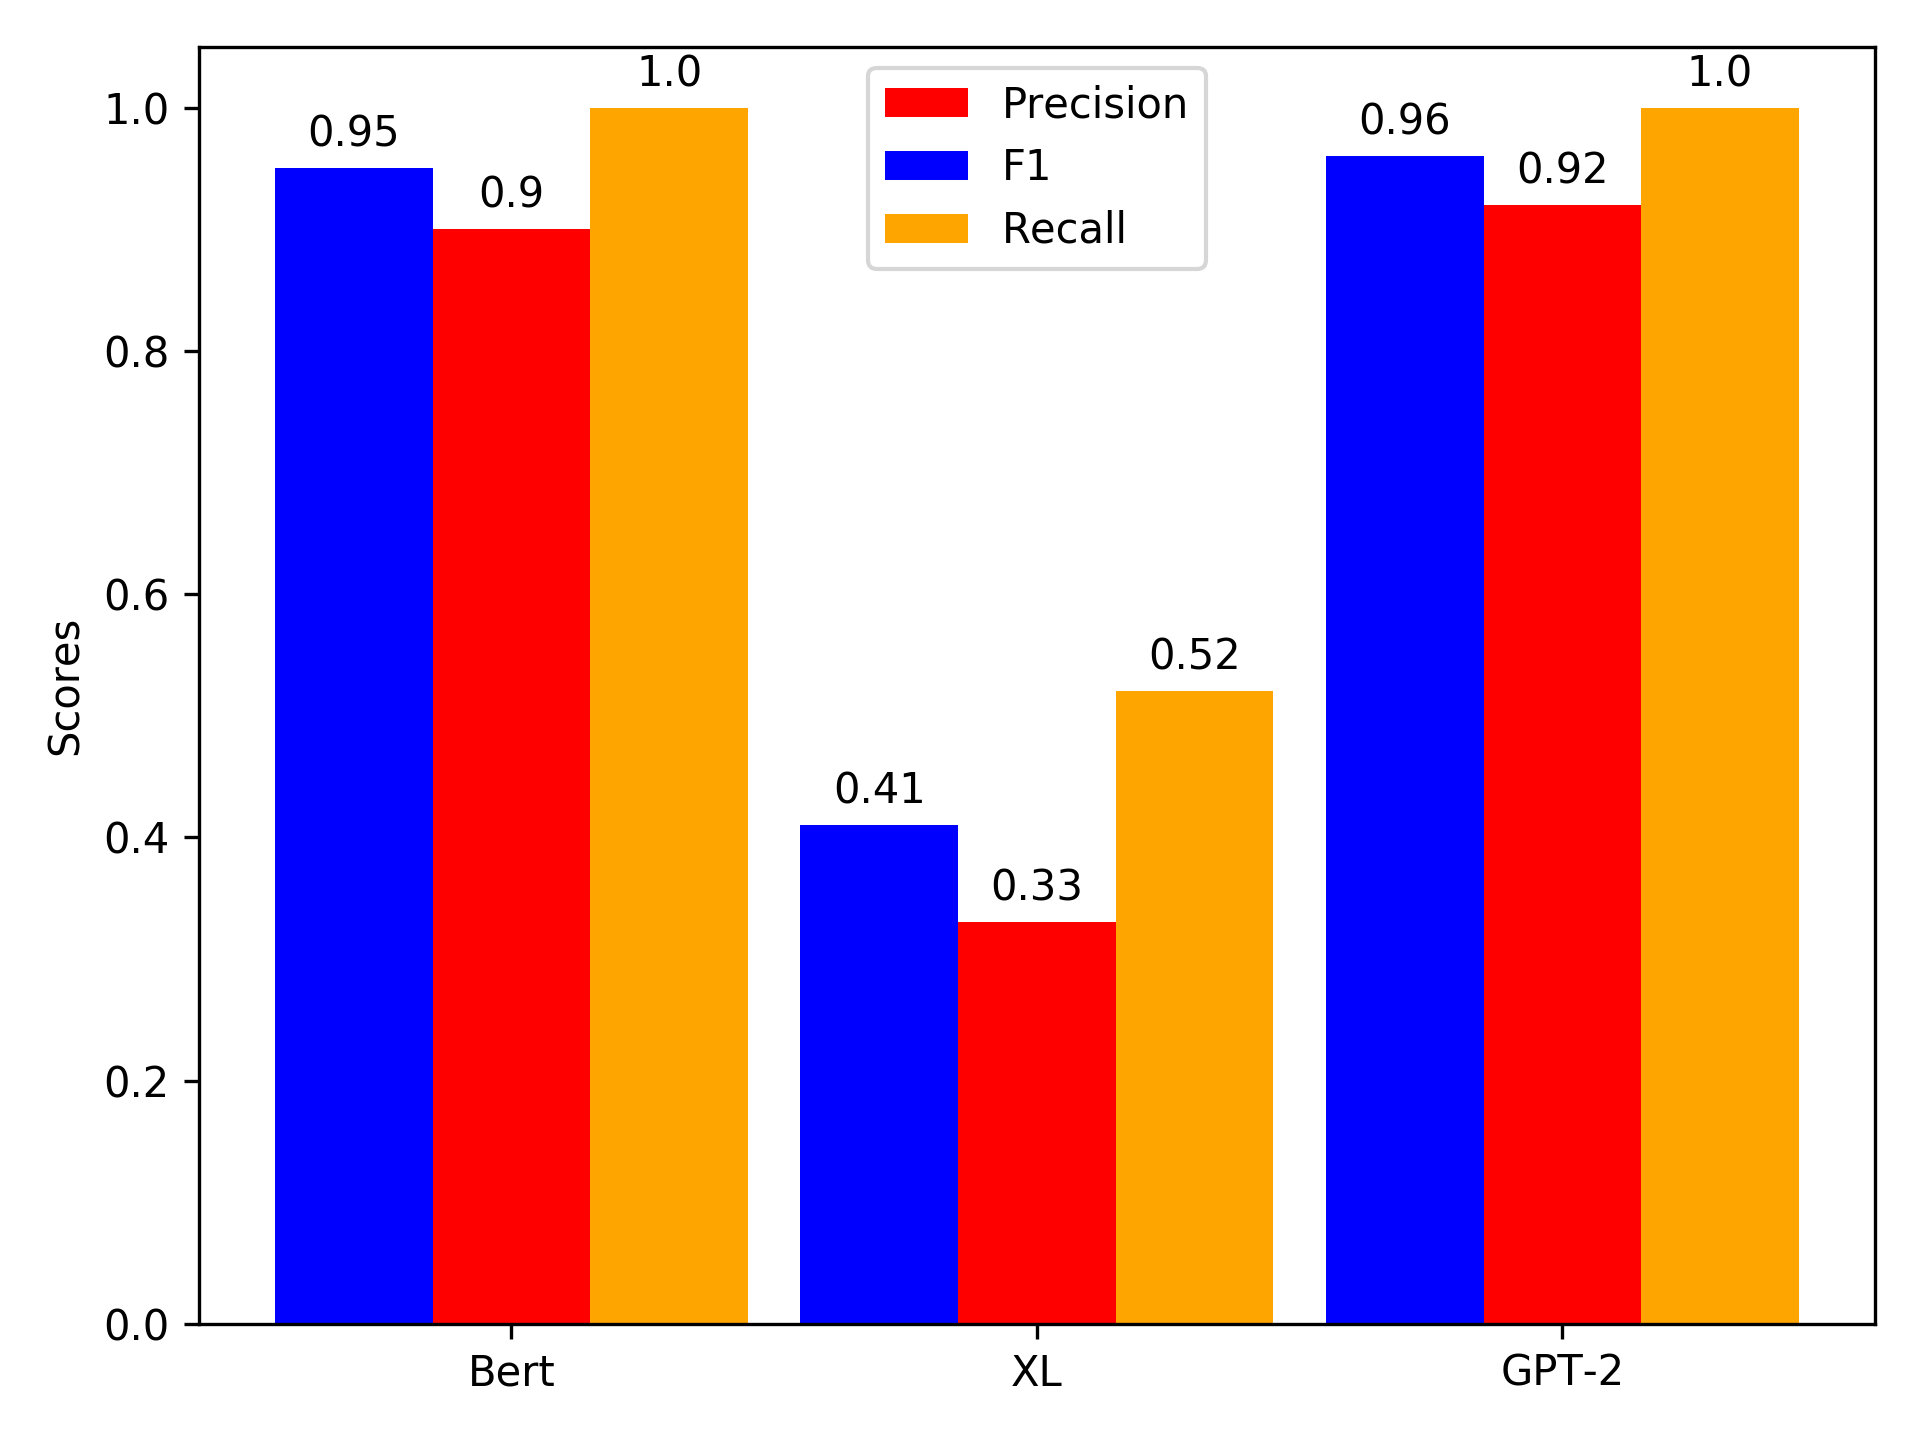
\includegraphics[trim={1cm 0.5cm 0cm 1cm}, width=0.322\textwidth]{results/transfer/transfer_regression_0.05_ratio.png}}
\hspace{\fill}
   \subfloat[10\% alteration\label{fig:results_transfer_regression_0.10} ]{%
      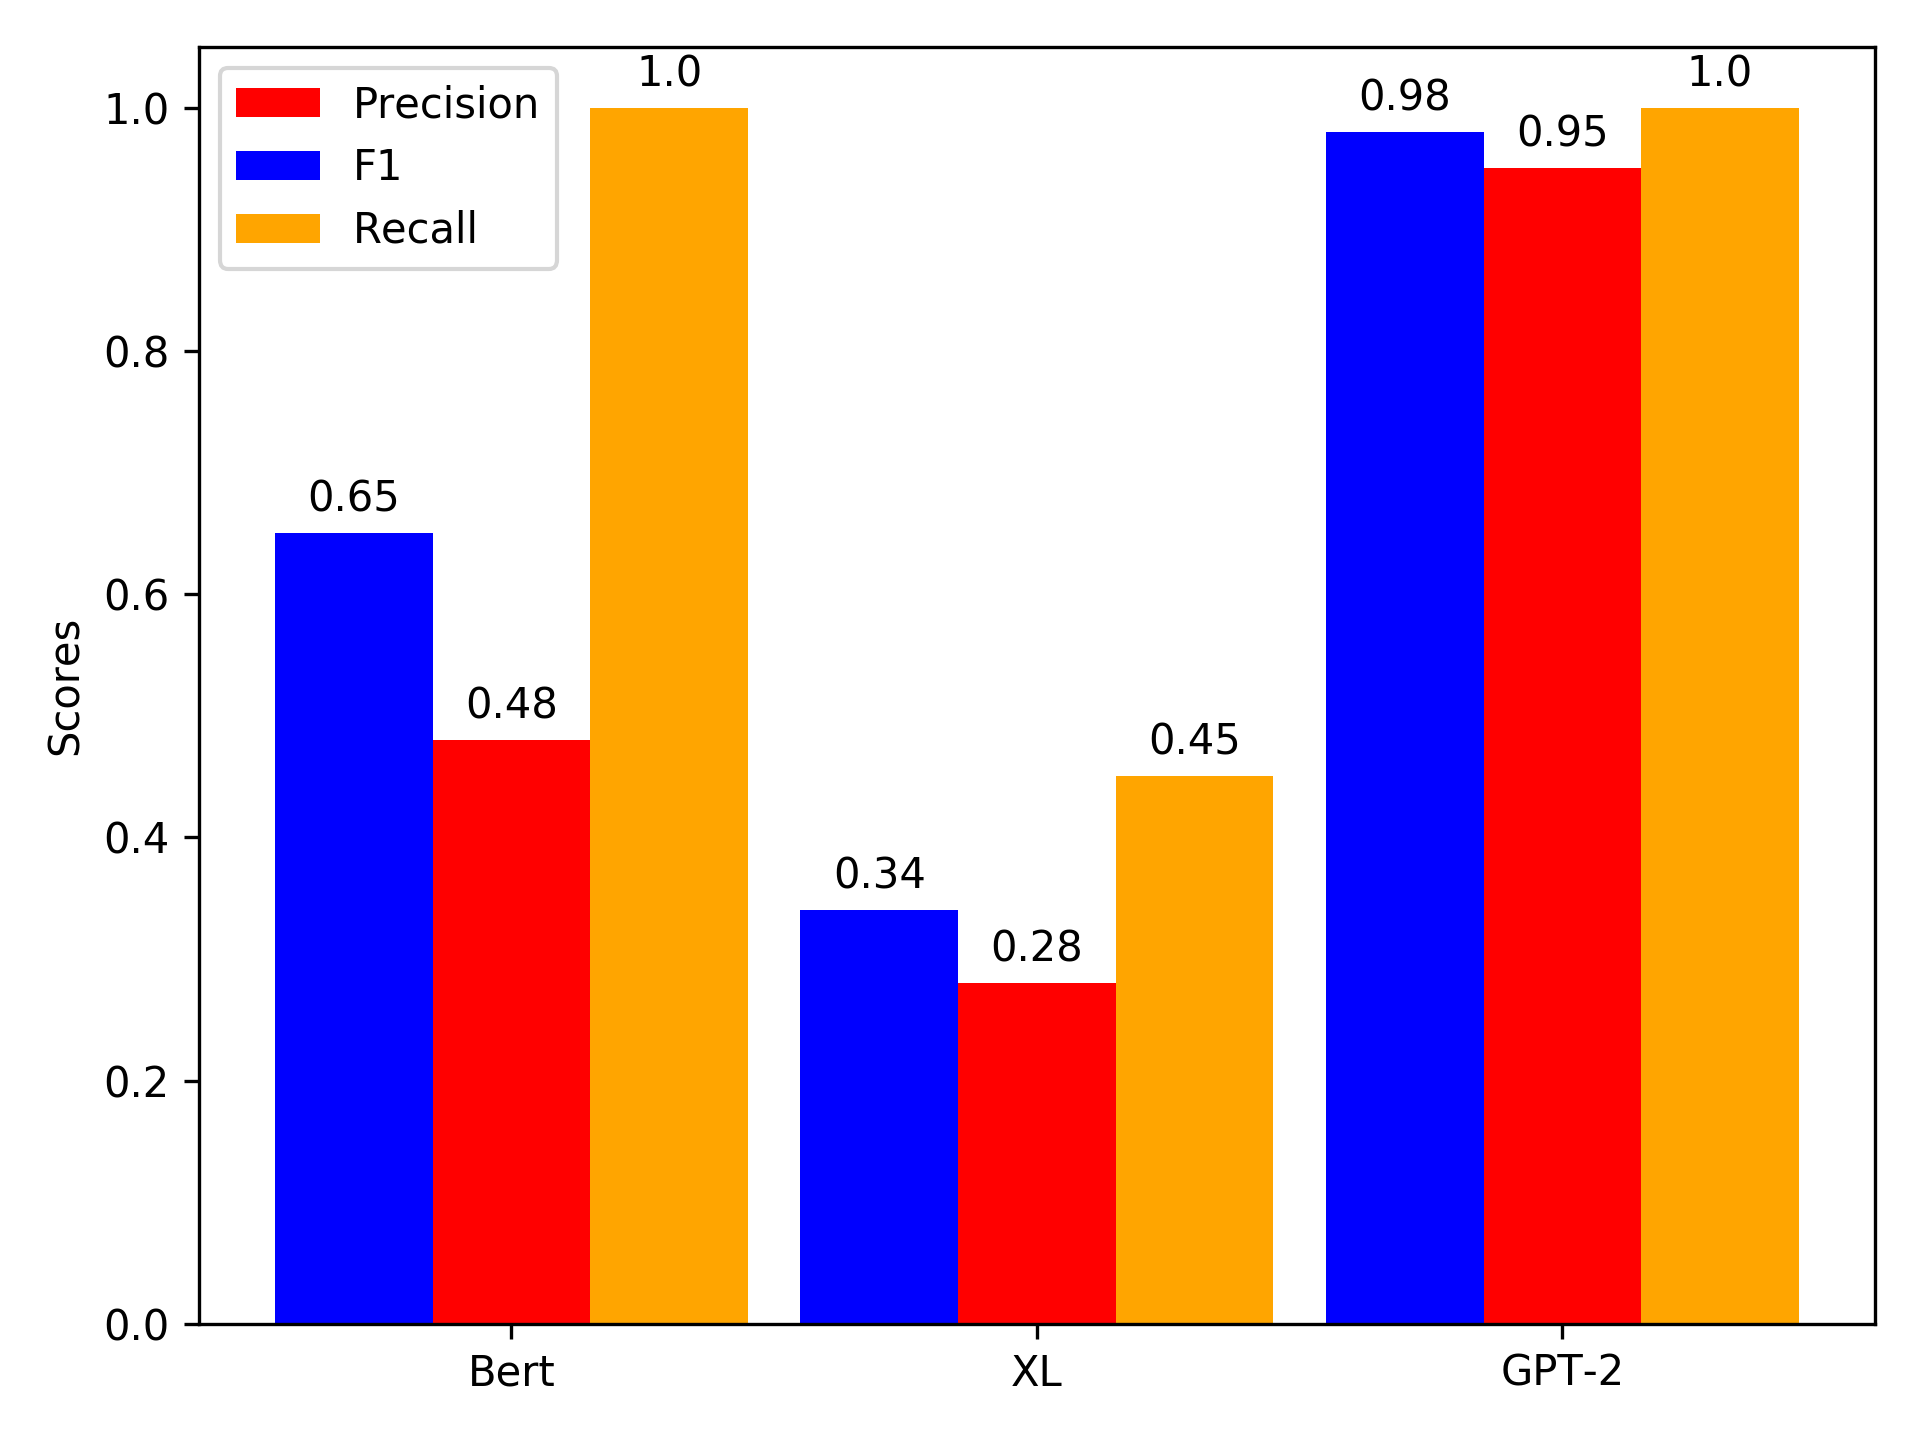
\includegraphics[trim={1cm 0.5cm 0cm 1cm}, width=0.322\textwidth]{results/transfer/transfer_regression_0.1_ratio.png}}
\hspace{\fill}
   \subfloat[15\% alteration\label{fig:results_transfer_regression_0.15}]{%
      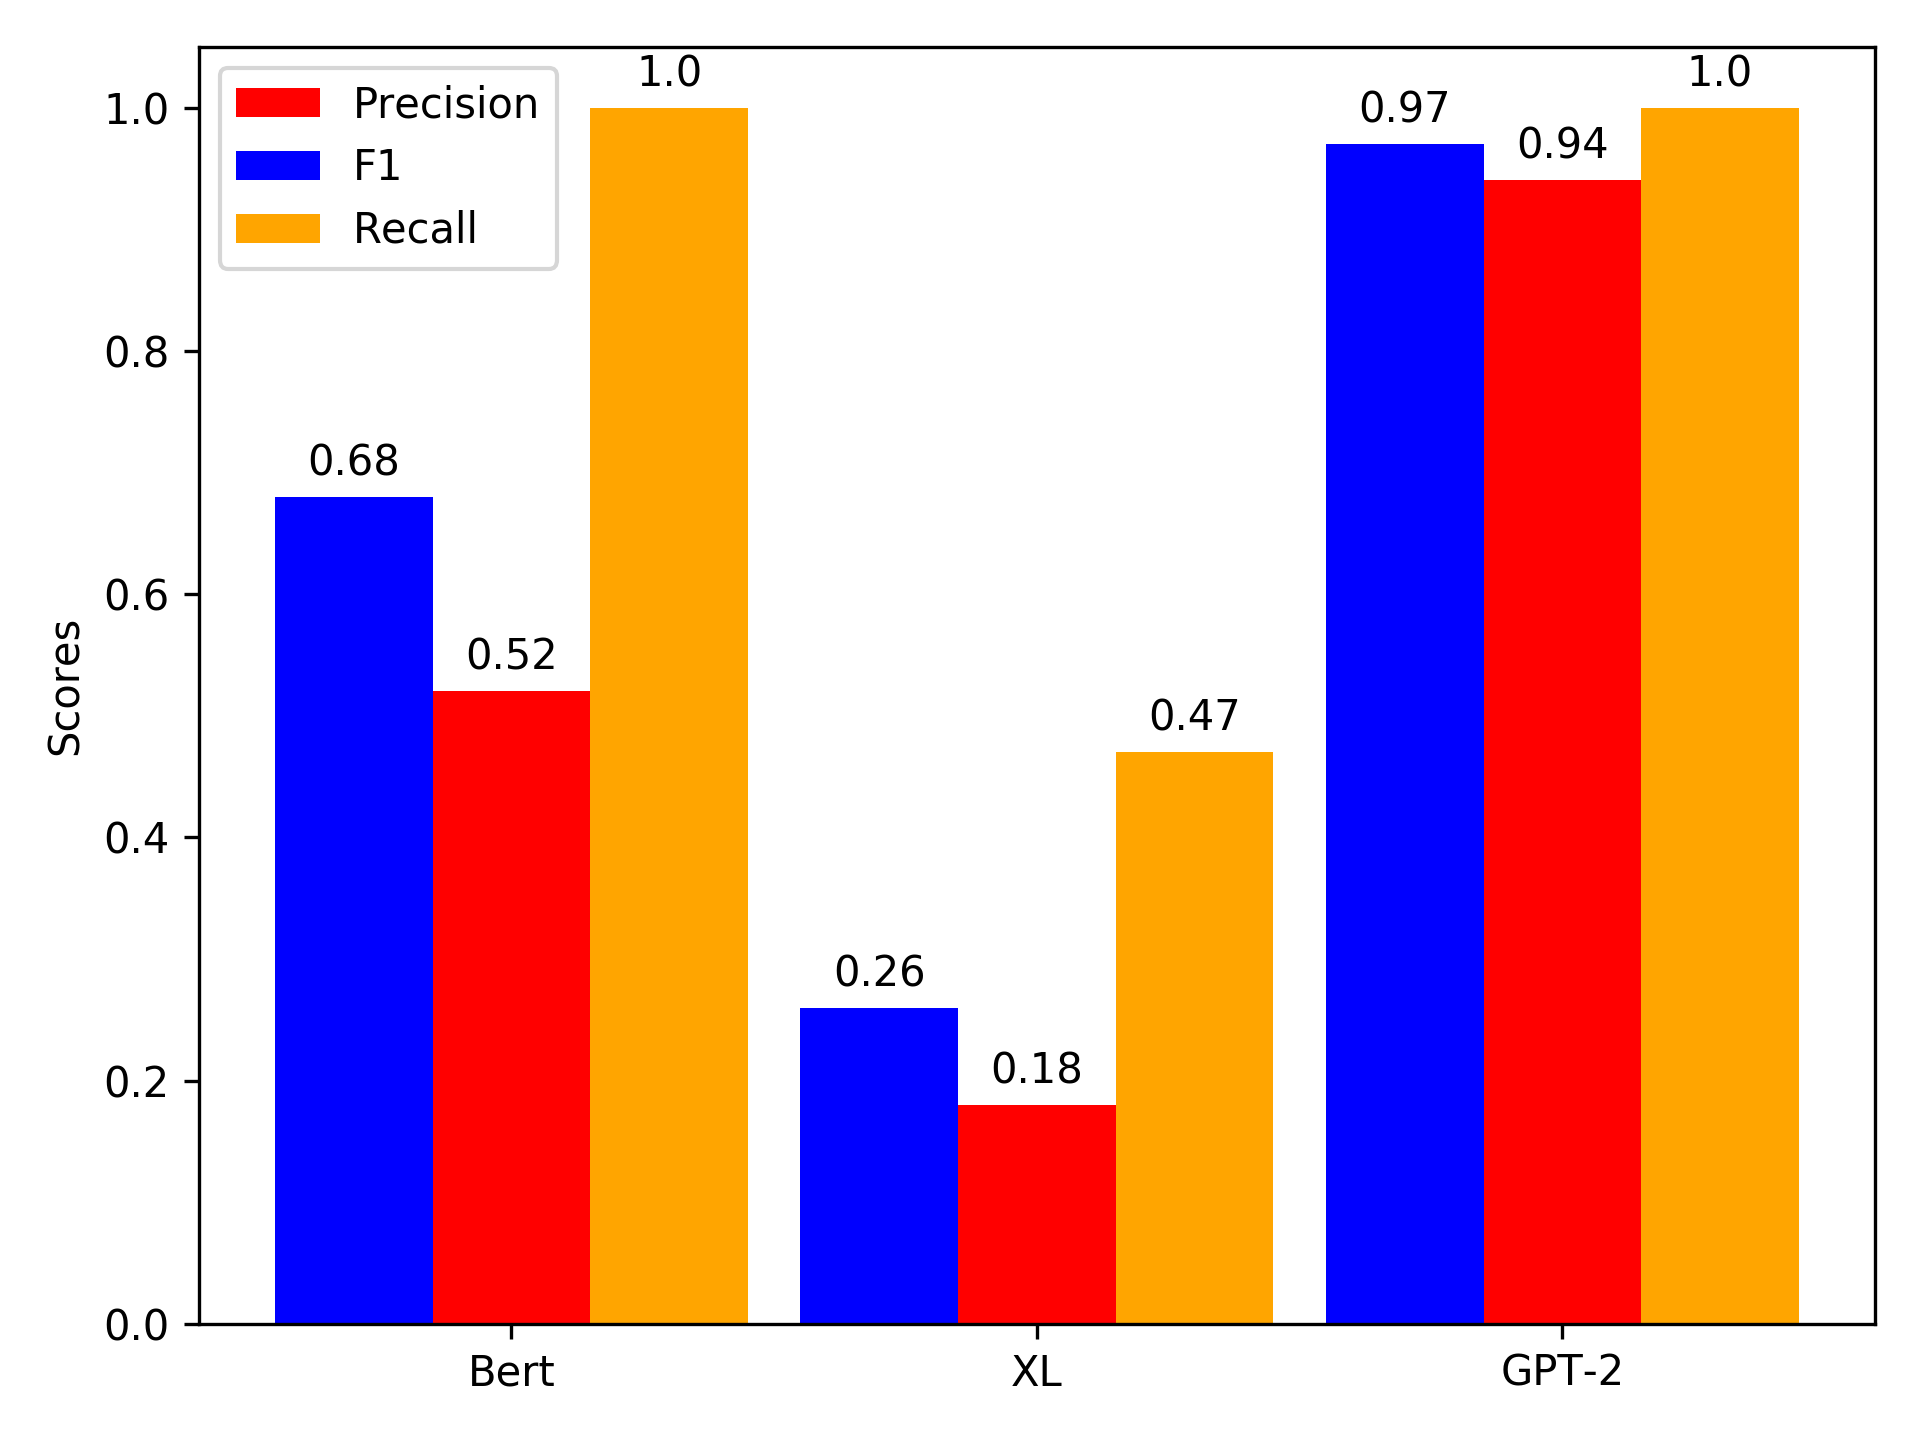
\includegraphics[trim={1cm 0.5cm 0cm 1cm}, width=0.322\textwidth]{results/transfer/transfer_regression_0.15_ratio.png}}\\
\caption{\label{fig:results_transfer_regression}Transfer learning with different ratios of alteration, using regression.}
\end{figure*}


Figure \ref{fig:results_transfer_regression_per_epoch} depicts the development of the metrics of detecting anomalies for every additional epoch of training on dataset B. It is clearly visible, that XL-Transformers improves the most per epoch, although starting from a relatively low starting point, whereas Bert has a smaller increase per training epoch. The results of GPT-2 do not change much per epoch, but start at a very high level already, corresponding to the findings already made on GPT-2 using regression in \ref{sec:results-regression}. These findings are confirmed by the ROC curve plots which can be seen in figure \ref{fig:results_transfer_regression_roc}, showing nearly perfect results for GPT-2, very good results for Bert and far less satisfying results for XL-Transformers.

\begin{figure*}[ht!]
   \subfloat[Bert\label{fig:results_transfer_regression_per_epoch_0.05}]{%
      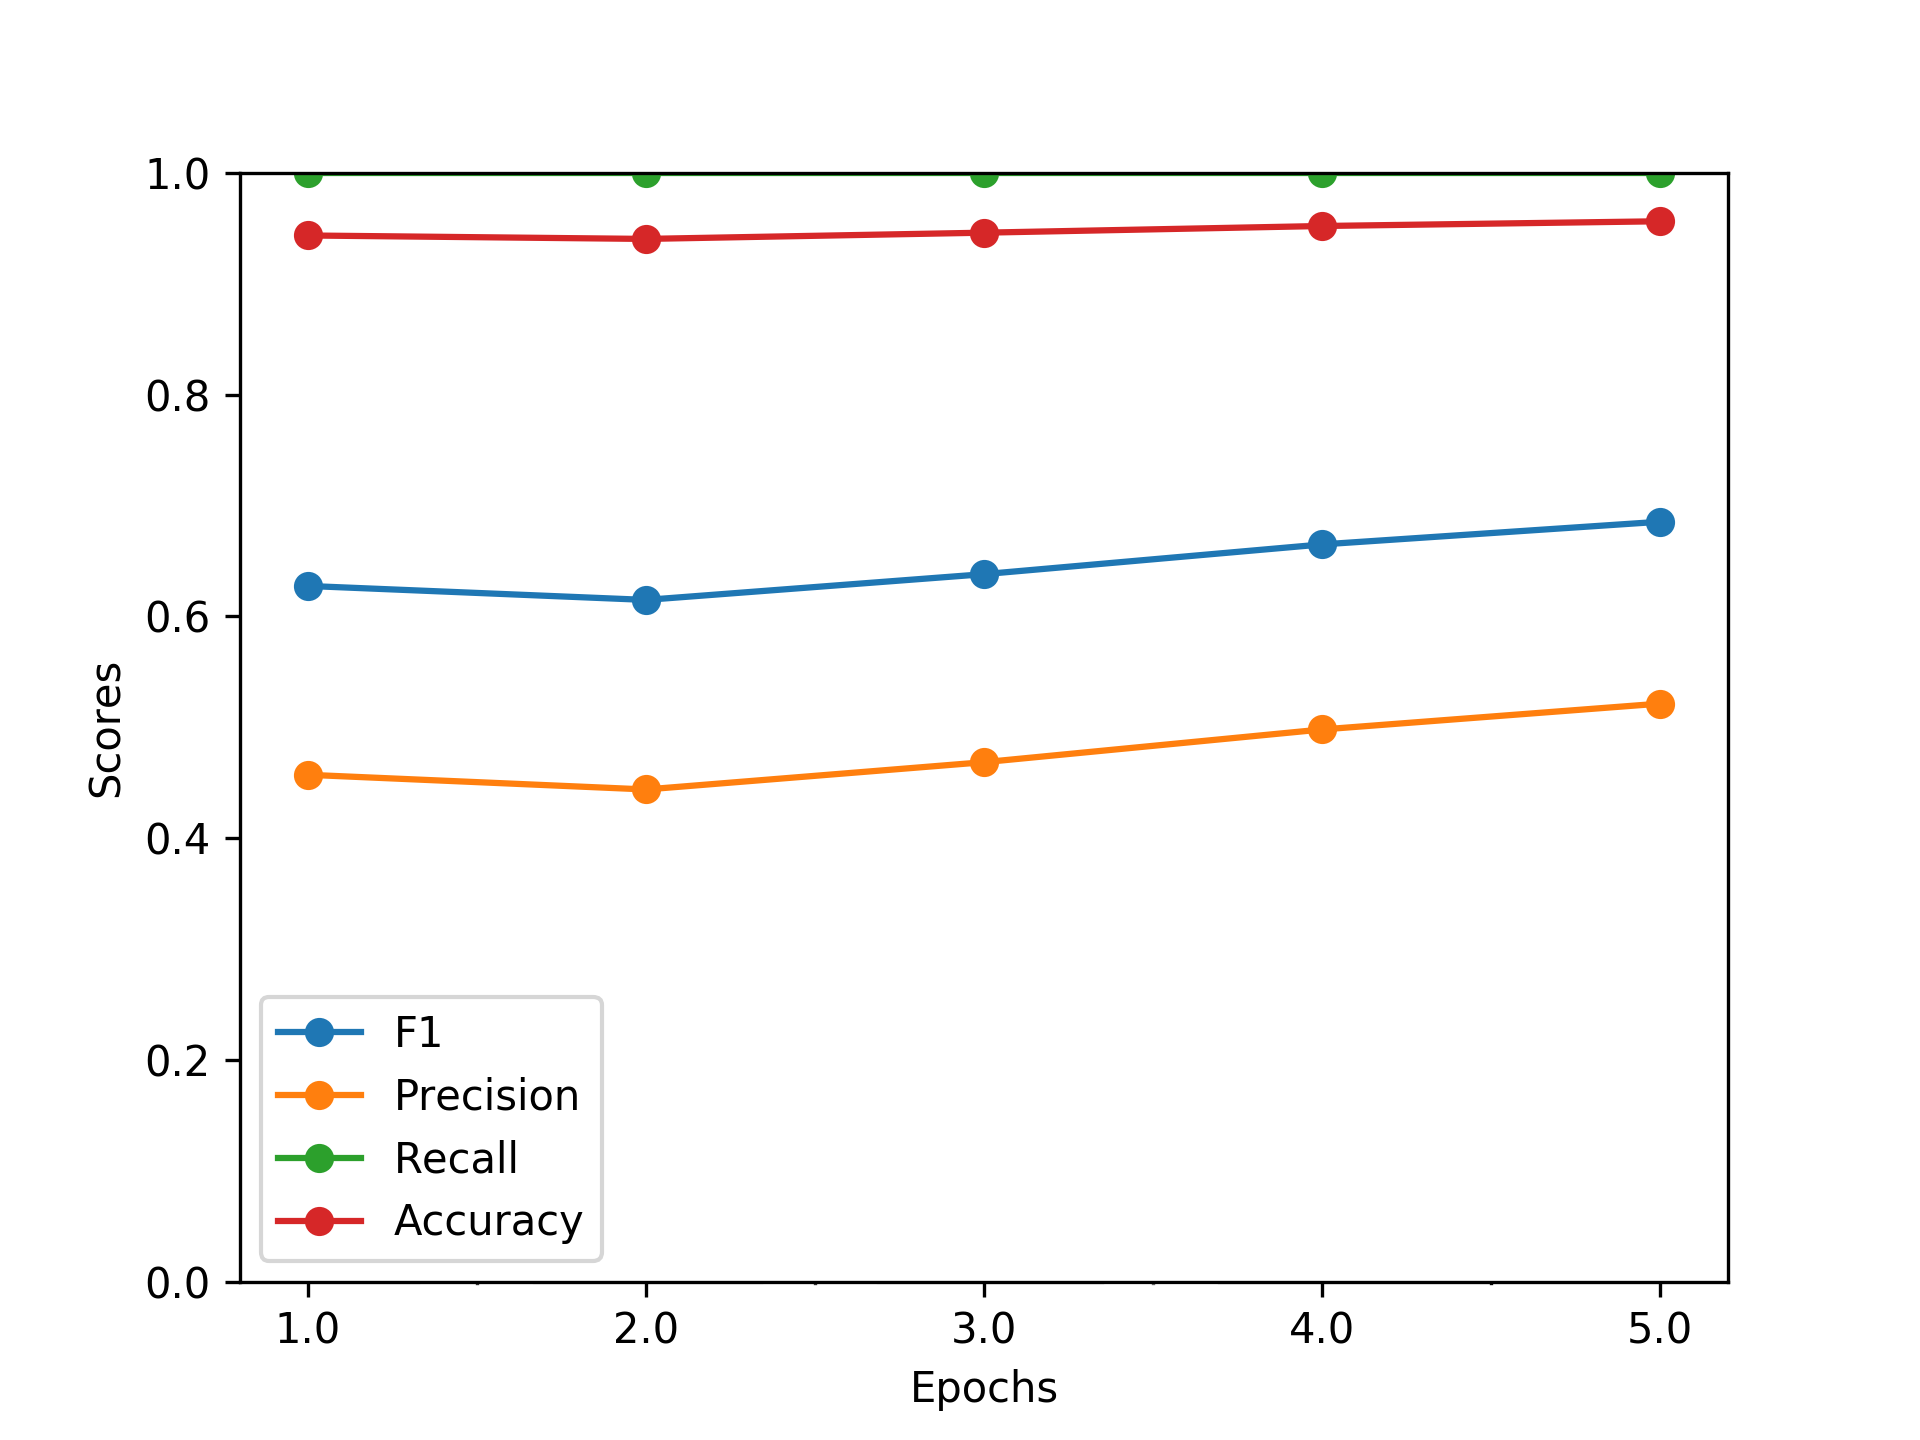
\includegraphics[trim={1cm 0.5cm 0cm 1cm}, width=0.322\textwidth]{results/transfer/bert_regression_0.15_transfer_metrics_per_epoch.png}}
\hspace{\fill}
   \subfloat[GPT-2\label{fig:results_transfer_regression_per_epoch_0.10} ]{%
      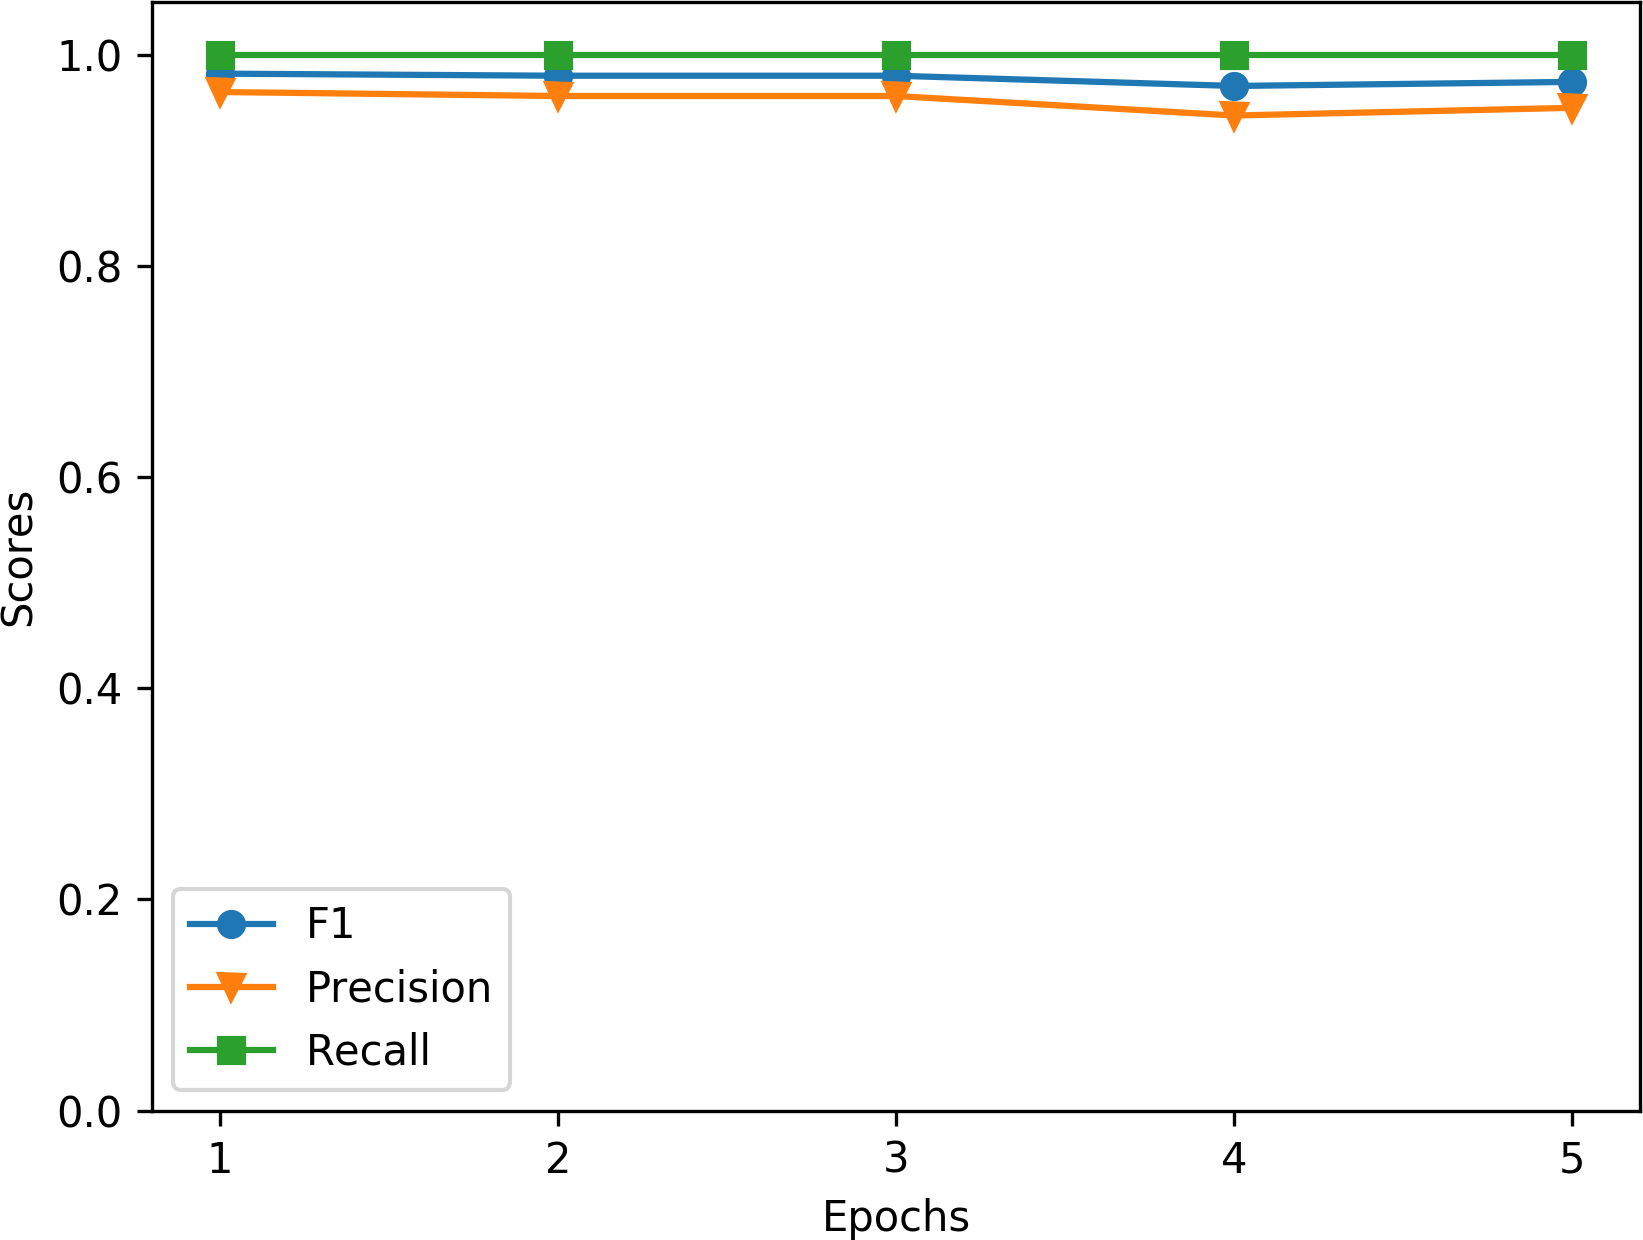
\includegraphics[trim={1cm 0.5cm 0cm 1cm}, width=0.322\textwidth]{results/transfer/gpt_regression_0.15_transfer_metrics_per_epoch.png}}
\hspace{\fill}
   \subfloat[XL\label{fig:results_transfer_regression_per_epoch_0.15}]{%
      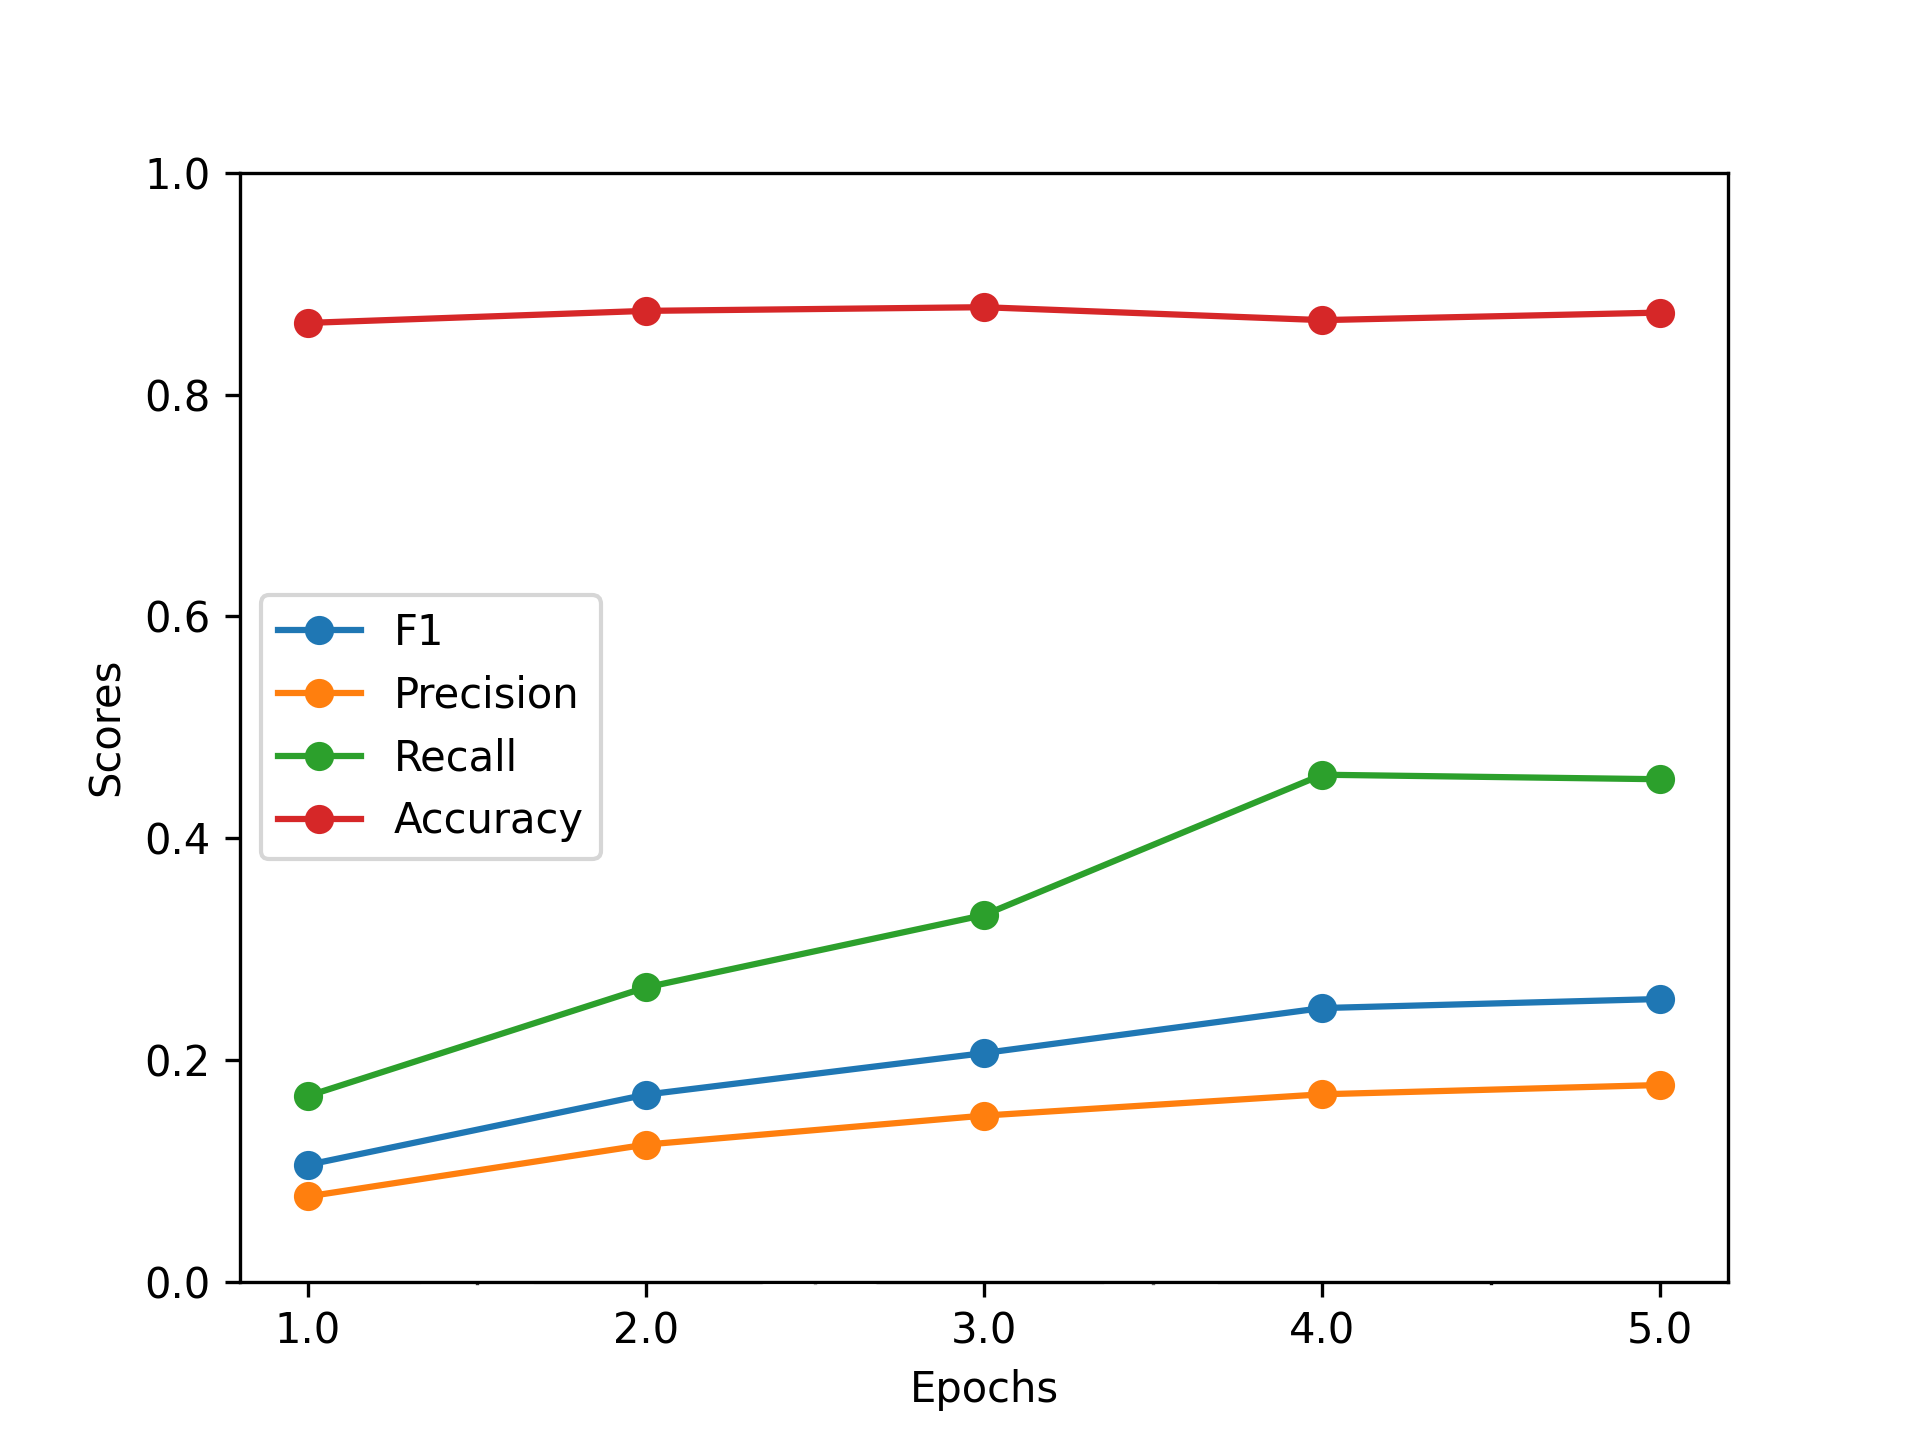
\includegraphics[trim={1cm 0.5cm 0cm 1cm}, width=0.322\textwidth]{results/transfer/xl_regression_0.15_transfer_metrics_per_epoch.png}}\\
\caption{\label{fig:results_transfer_regression_per_epoch}Improvement of metrics per additional learning epoch, using regression.}
\end{figure*}


\begin{figure*}[ht!]
   \subfloat[Bert\label{fig:roc_curve_bert_transfer_regression}]{%
      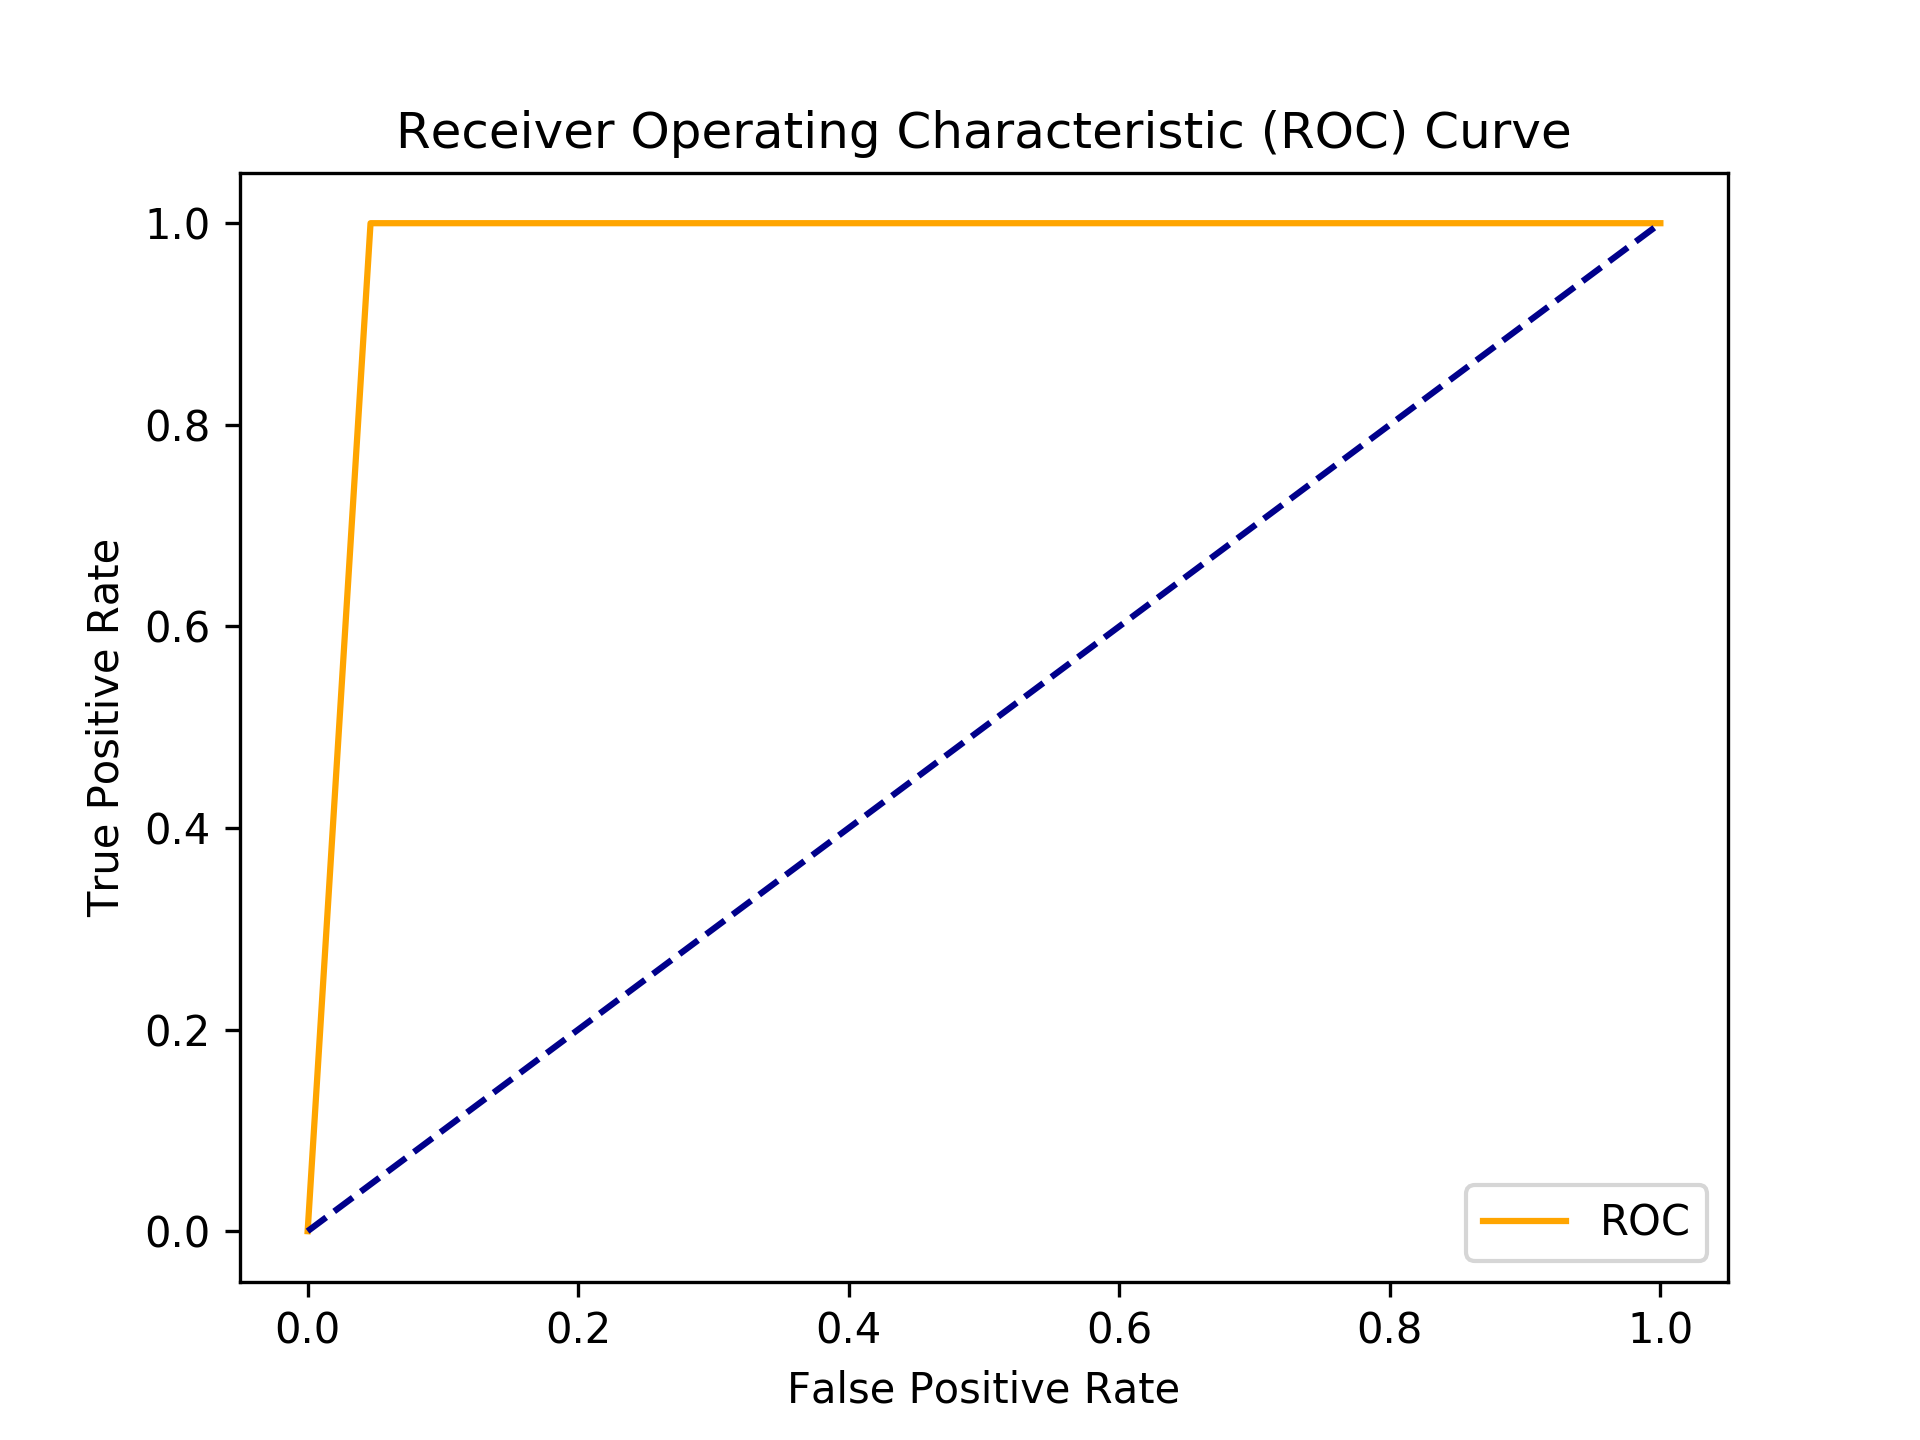
\includegraphics[trim={1cm 0.5cm 0cm 1cm}, width=0.322\textwidth]{results/transfer/roc_curve_transfer_regression_bert_0.15.png}}
\hspace{\fill}
   \subfloat[GPT-2\label{fig:roc_curve_gpt_transfer_regression} ]{%
      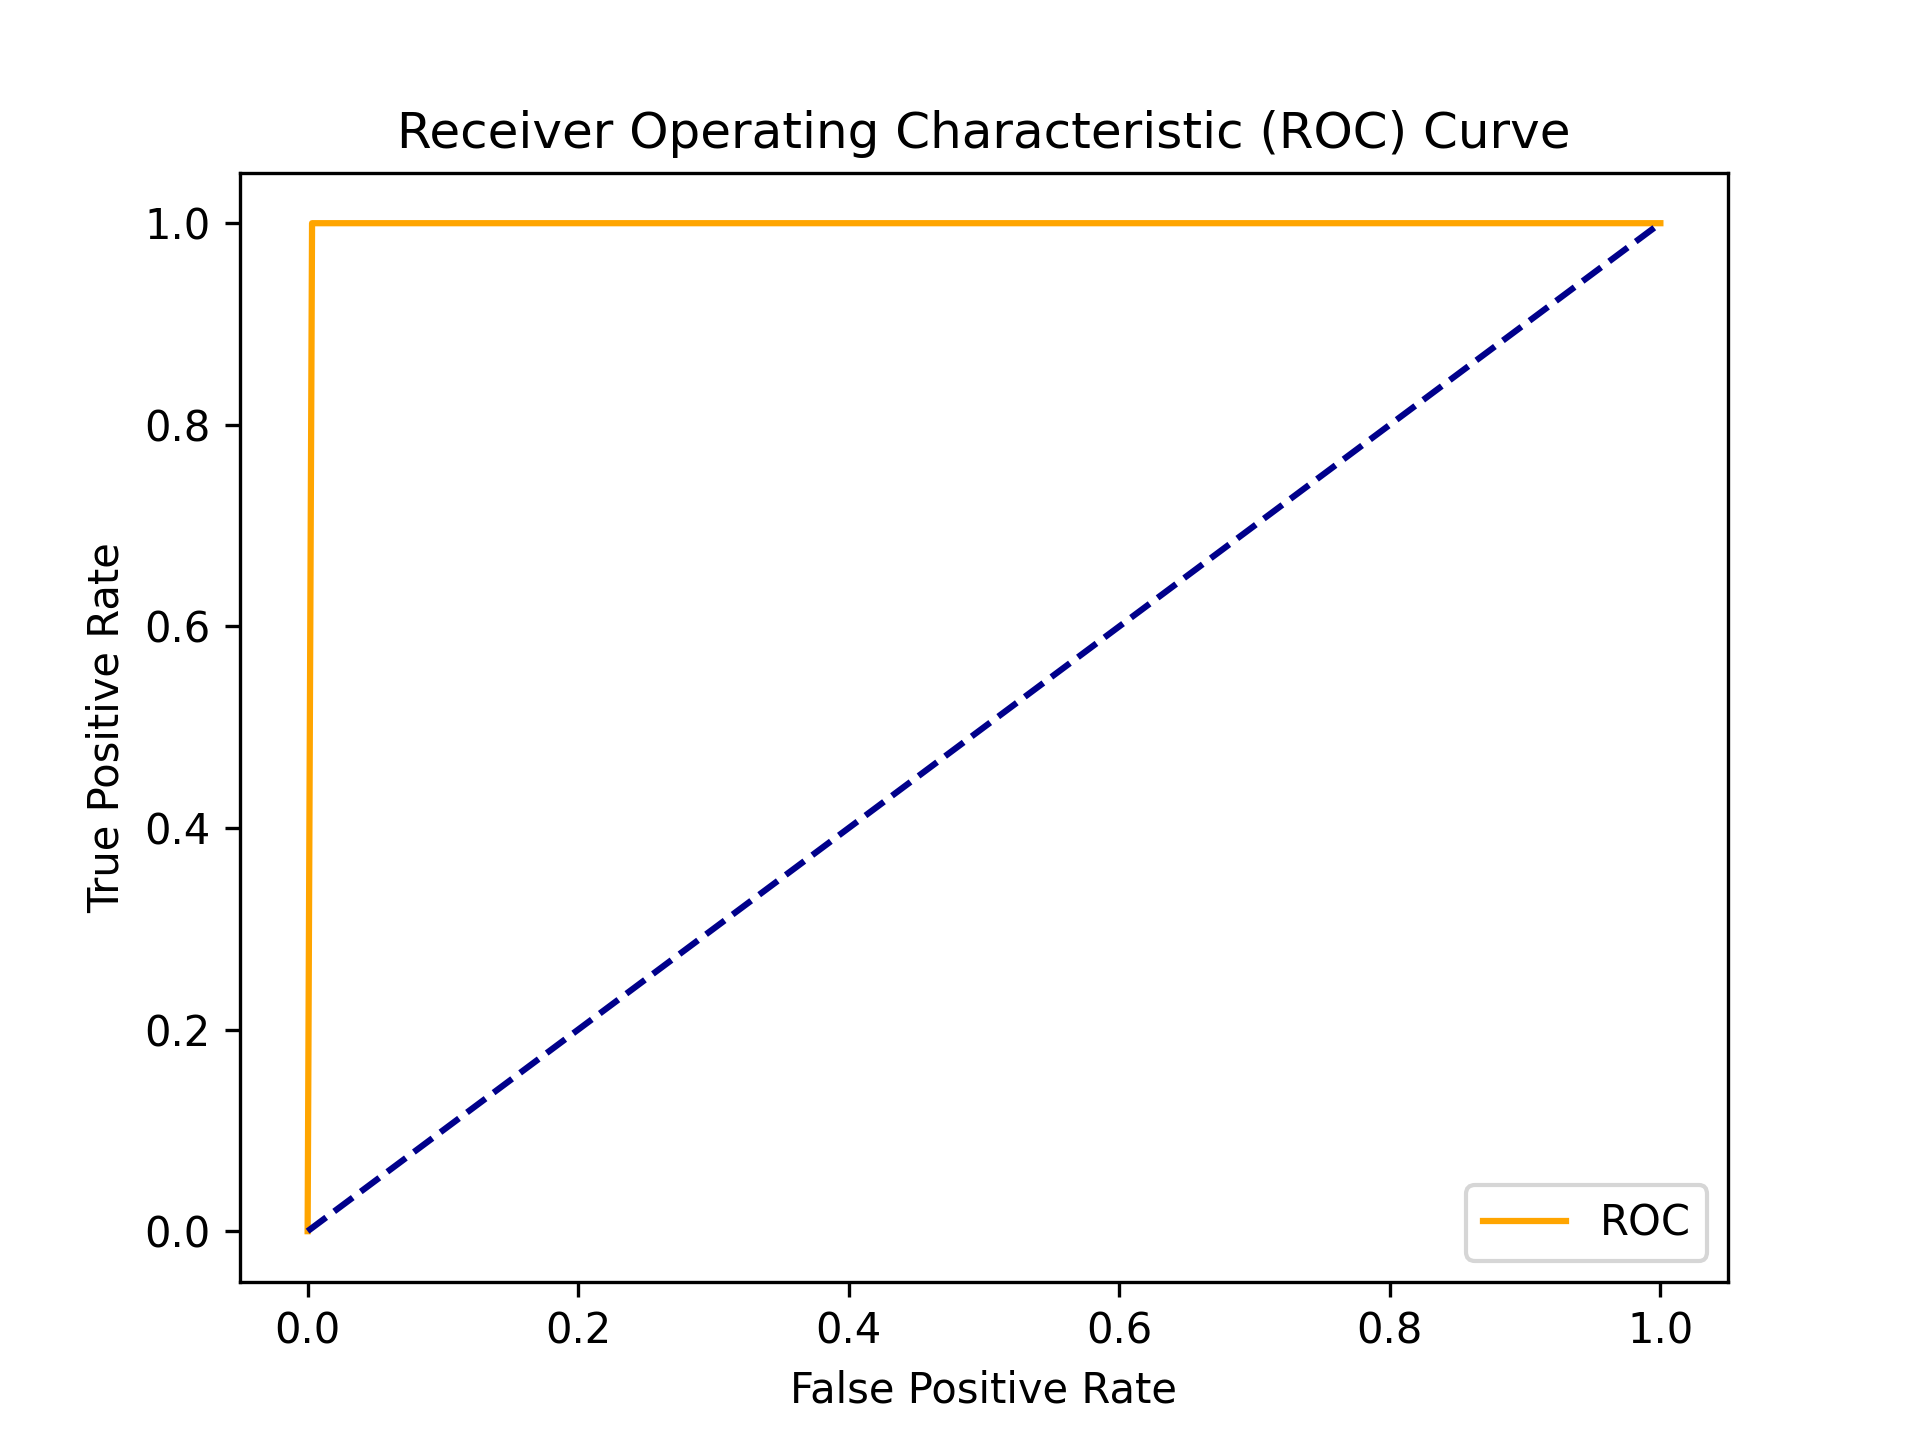
\includegraphics[trim={1cm 0.5cm 0cm 1cm}, width=0.322\textwidth]{results/transfer/roc_curve_transfer_regression_gpt_0.15.png}}
\hspace{\fill}
   \subfloat[XL\label{fig:roc_curve_xl_transfer_regression}]{%
      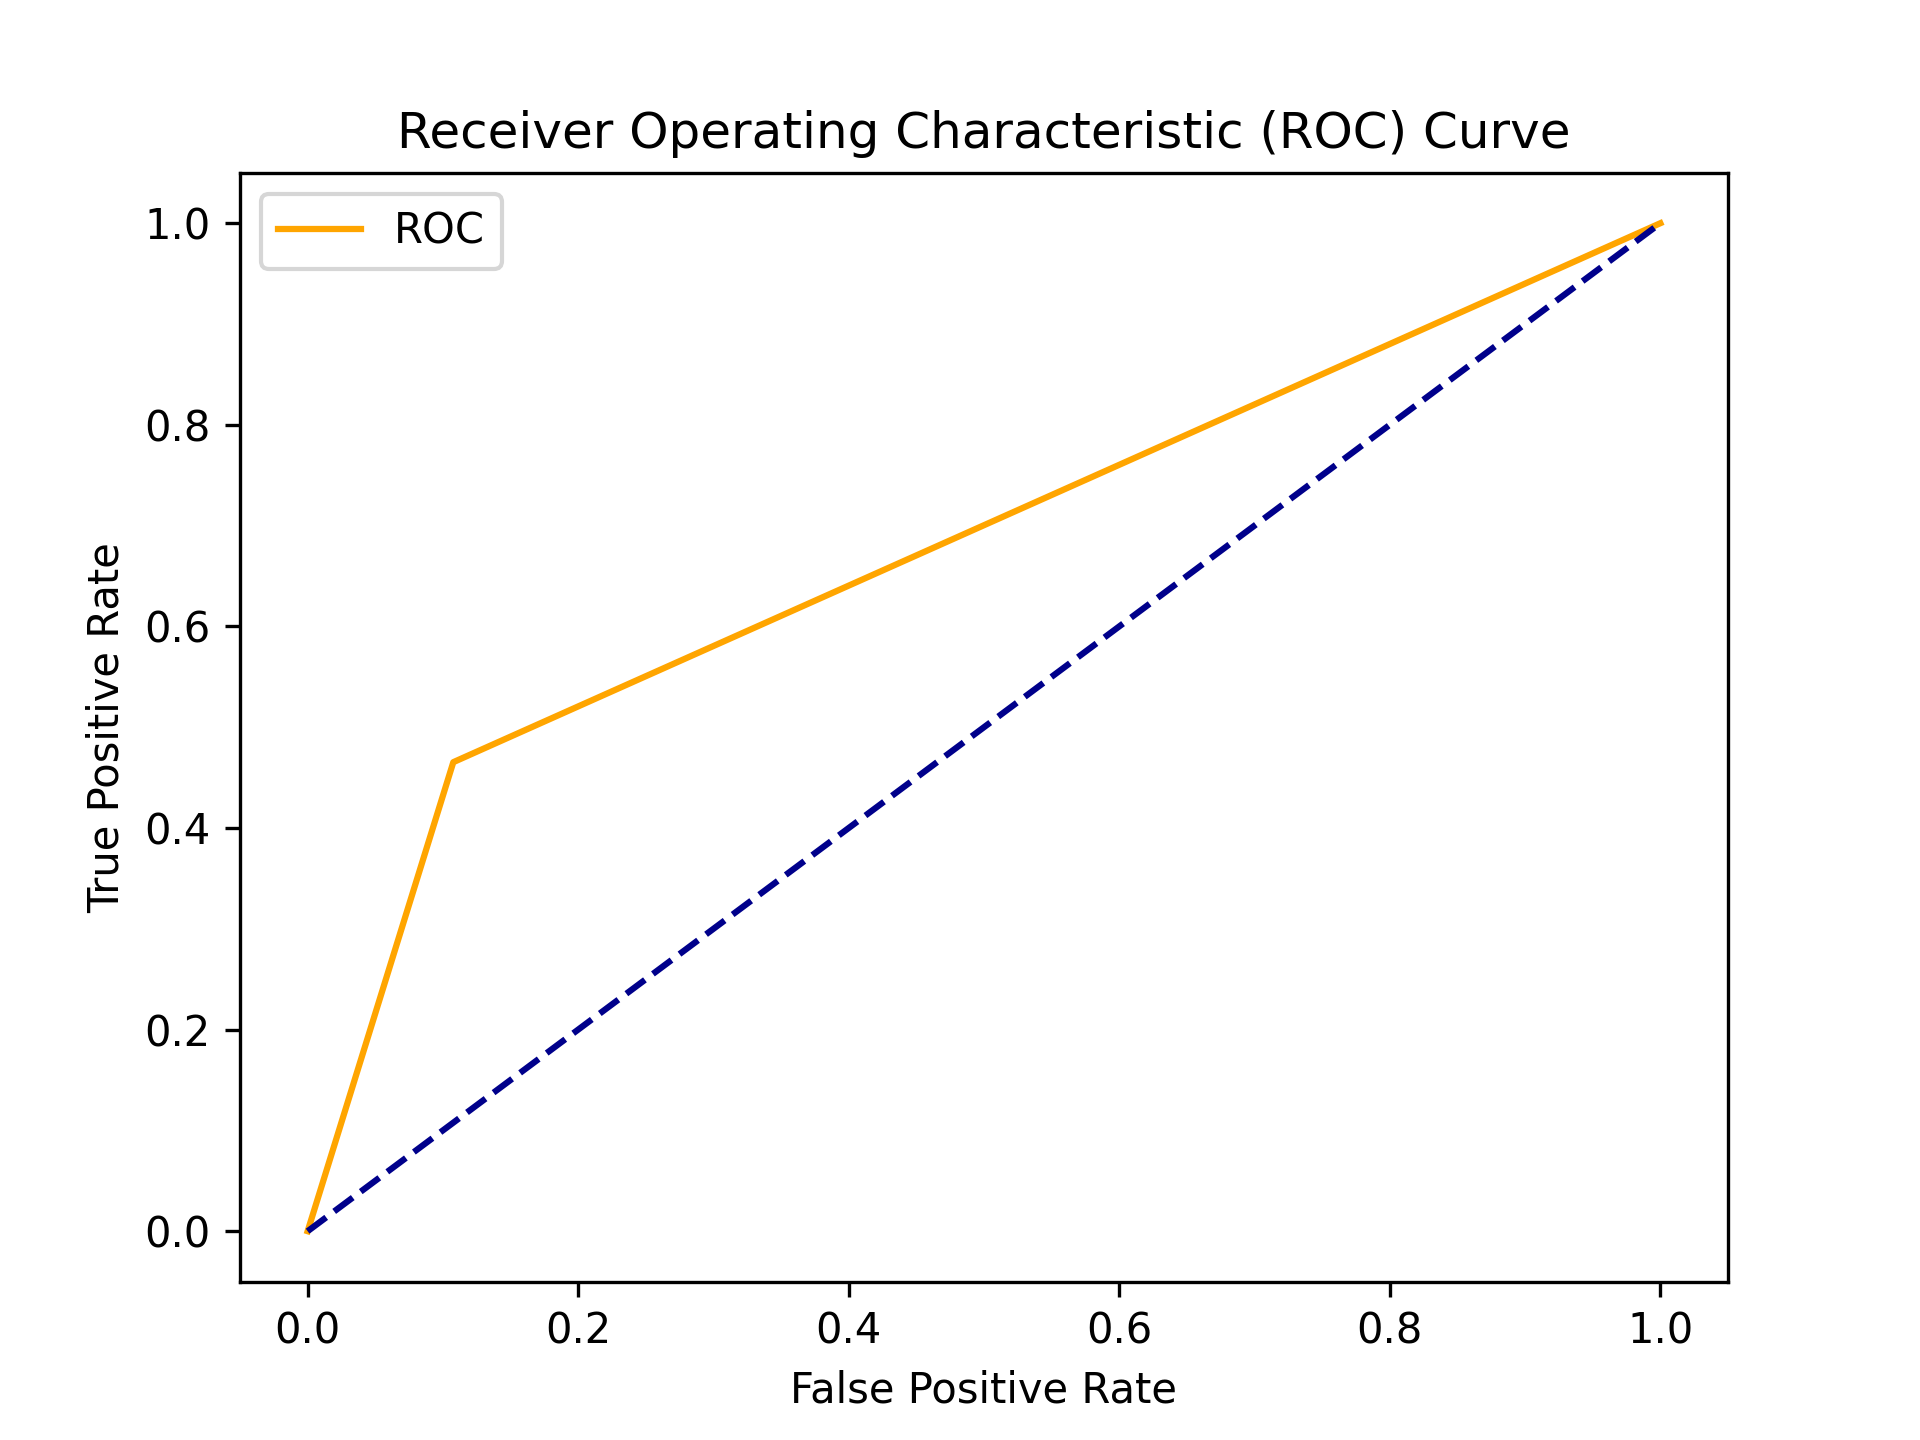
\includegraphics[trim={1cm 0.5cm 0cm 1cm}, width=0.322\textwidth]{results/transfer/roc_curve_transfer_regression_xl_0.15.png}}\\
\caption{\label{fig:results_transfer_regression_roc}ROC-Curve for transfer learning using regression with 15\% alterations.}
\end{figure*}



%%%% TRANSFER LEARNING CLASSIFICATION
\subsubsection{Transfer learning using the classification-based approach \label{sec:results-classification-transfer}}

For transfer learning using the classification-based approach, the same experiments as described in \ref{sec:results-regression-transfer} were conducted. Figure \ref{fig:results_transfer_classification} shows the results of the transfer learning experiment. Interesting observations include the stable results achieved using Bert, which are little sensitive to increasing alteration ratios and the results of GPT-2, which are not as useful as compared to the regression-based approach.
Figure \ref{fig:results_transfer_multiclass_per_epoch} depicts the development of the metrics of detecting anomalies for every additional epoch of training on dataset B. Bert improves the most per epoch, ramping up steeply after epoch 5 is completed, GPT-2 stays almost the same and XL-Transformers has small improvements over the course of the 5 epochs. These findings are confirmed by the ROC curve plots which can be seen in figure \ref{fig:results_transfer_multiclass_roc}, showing very good results for Bert,  acceptable results for Xl-Transformers and far less satisfying results for GPT-2.

\begin{figure*}[ht!]
   \subfloat[5\% alteration\label{fig:results_transfer_classification_0.05}]{%
      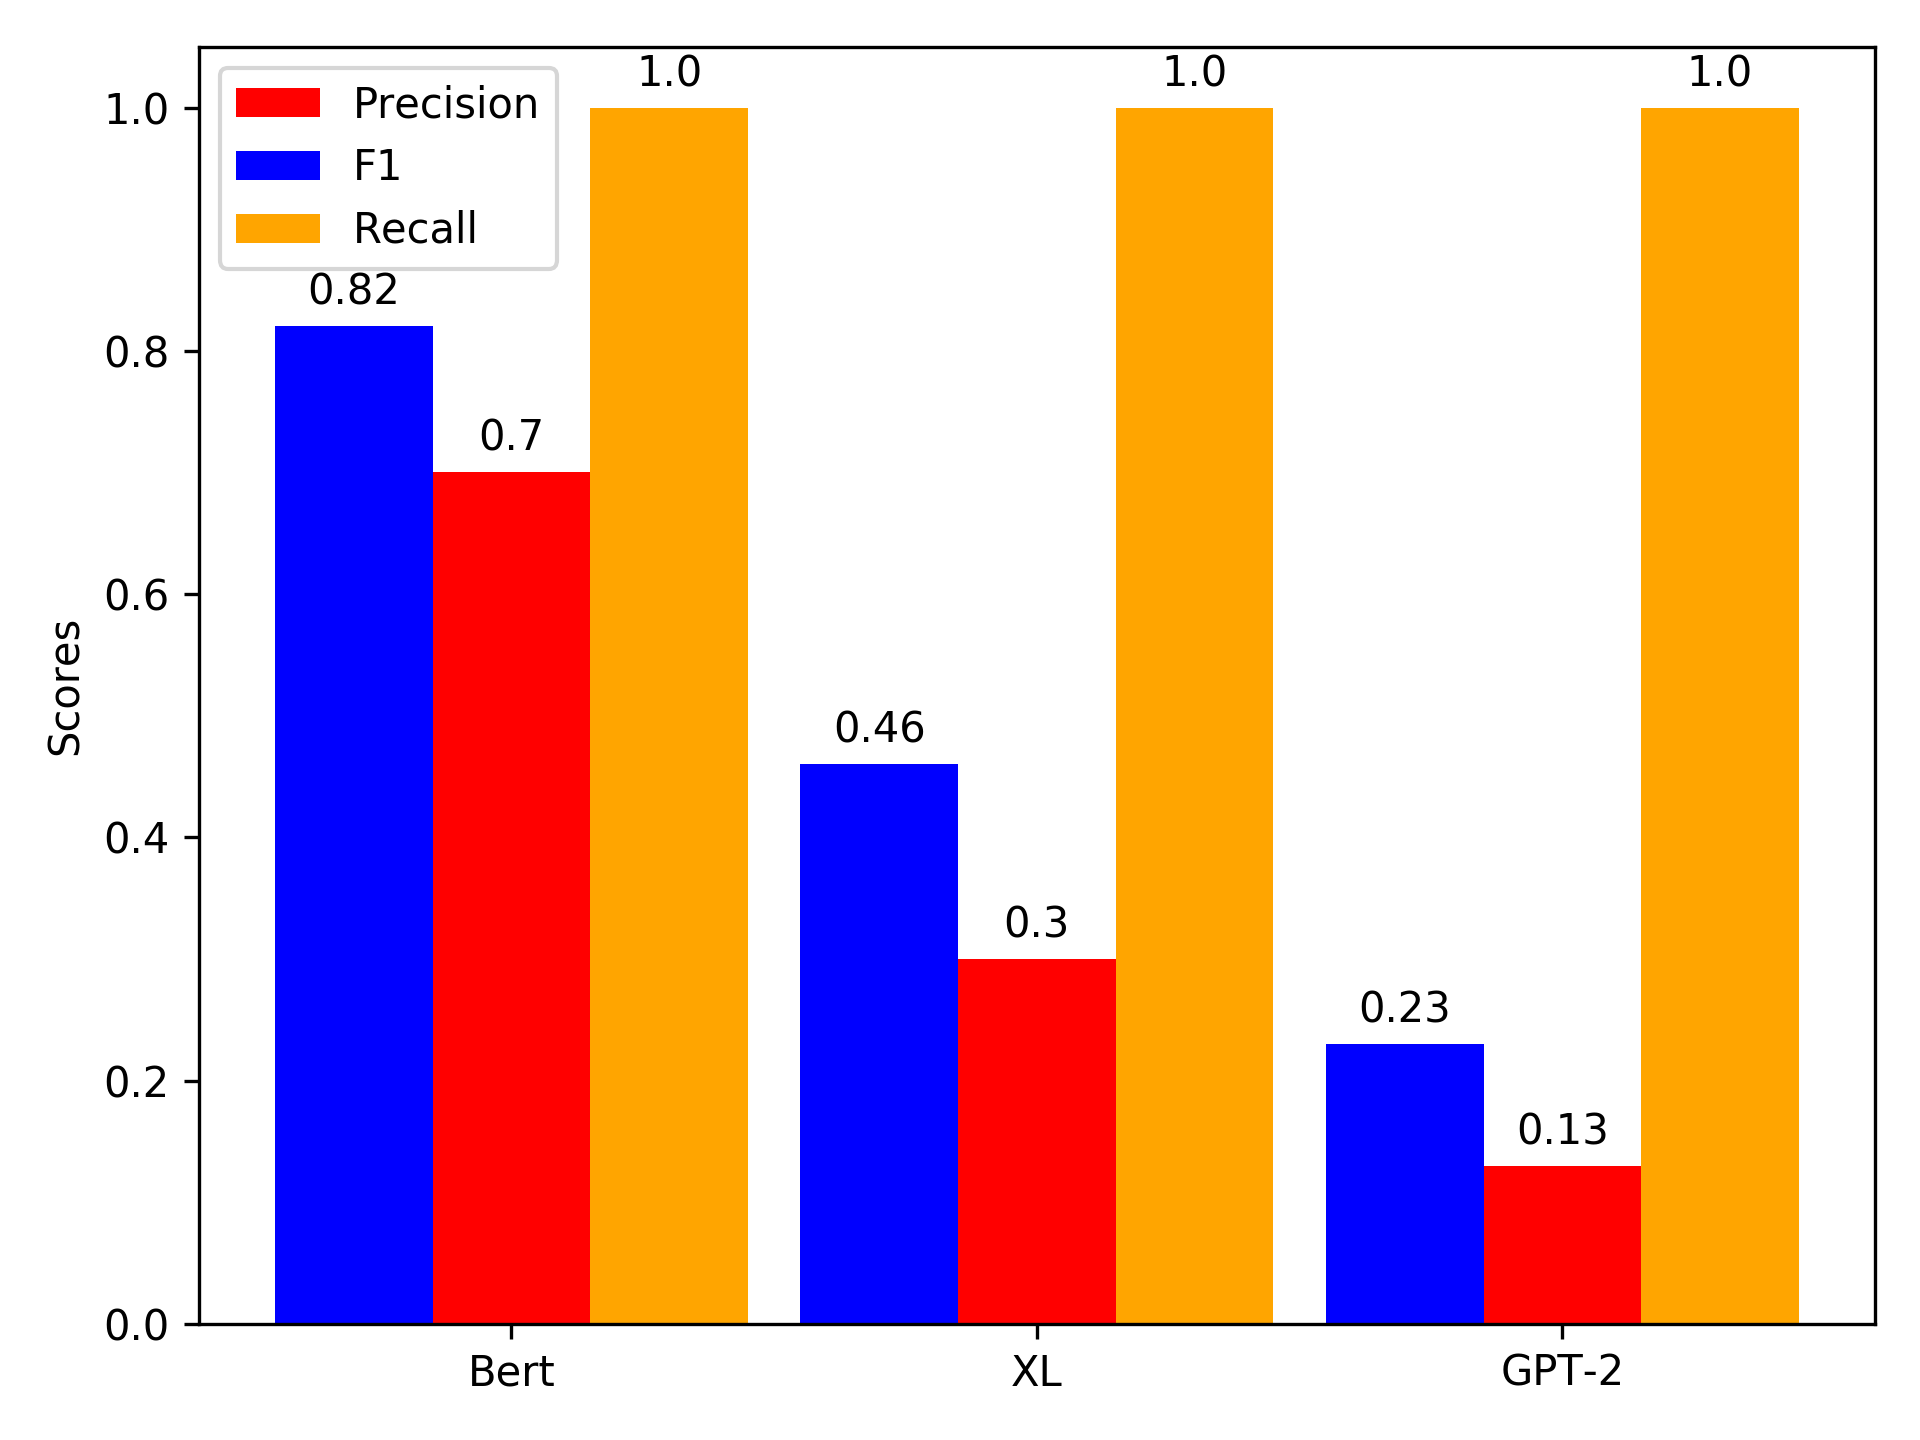
\includegraphics[trim={1cm 0.5cm 0cm 1cm}, width=0.322\textwidth]{results/transfer/transfer_multiclass_0.05_ratio.png}}
\hspace{\fill}
   \subfloat[10\% alteration\label{fig:results_transfer_classification_0.10} ]{%
      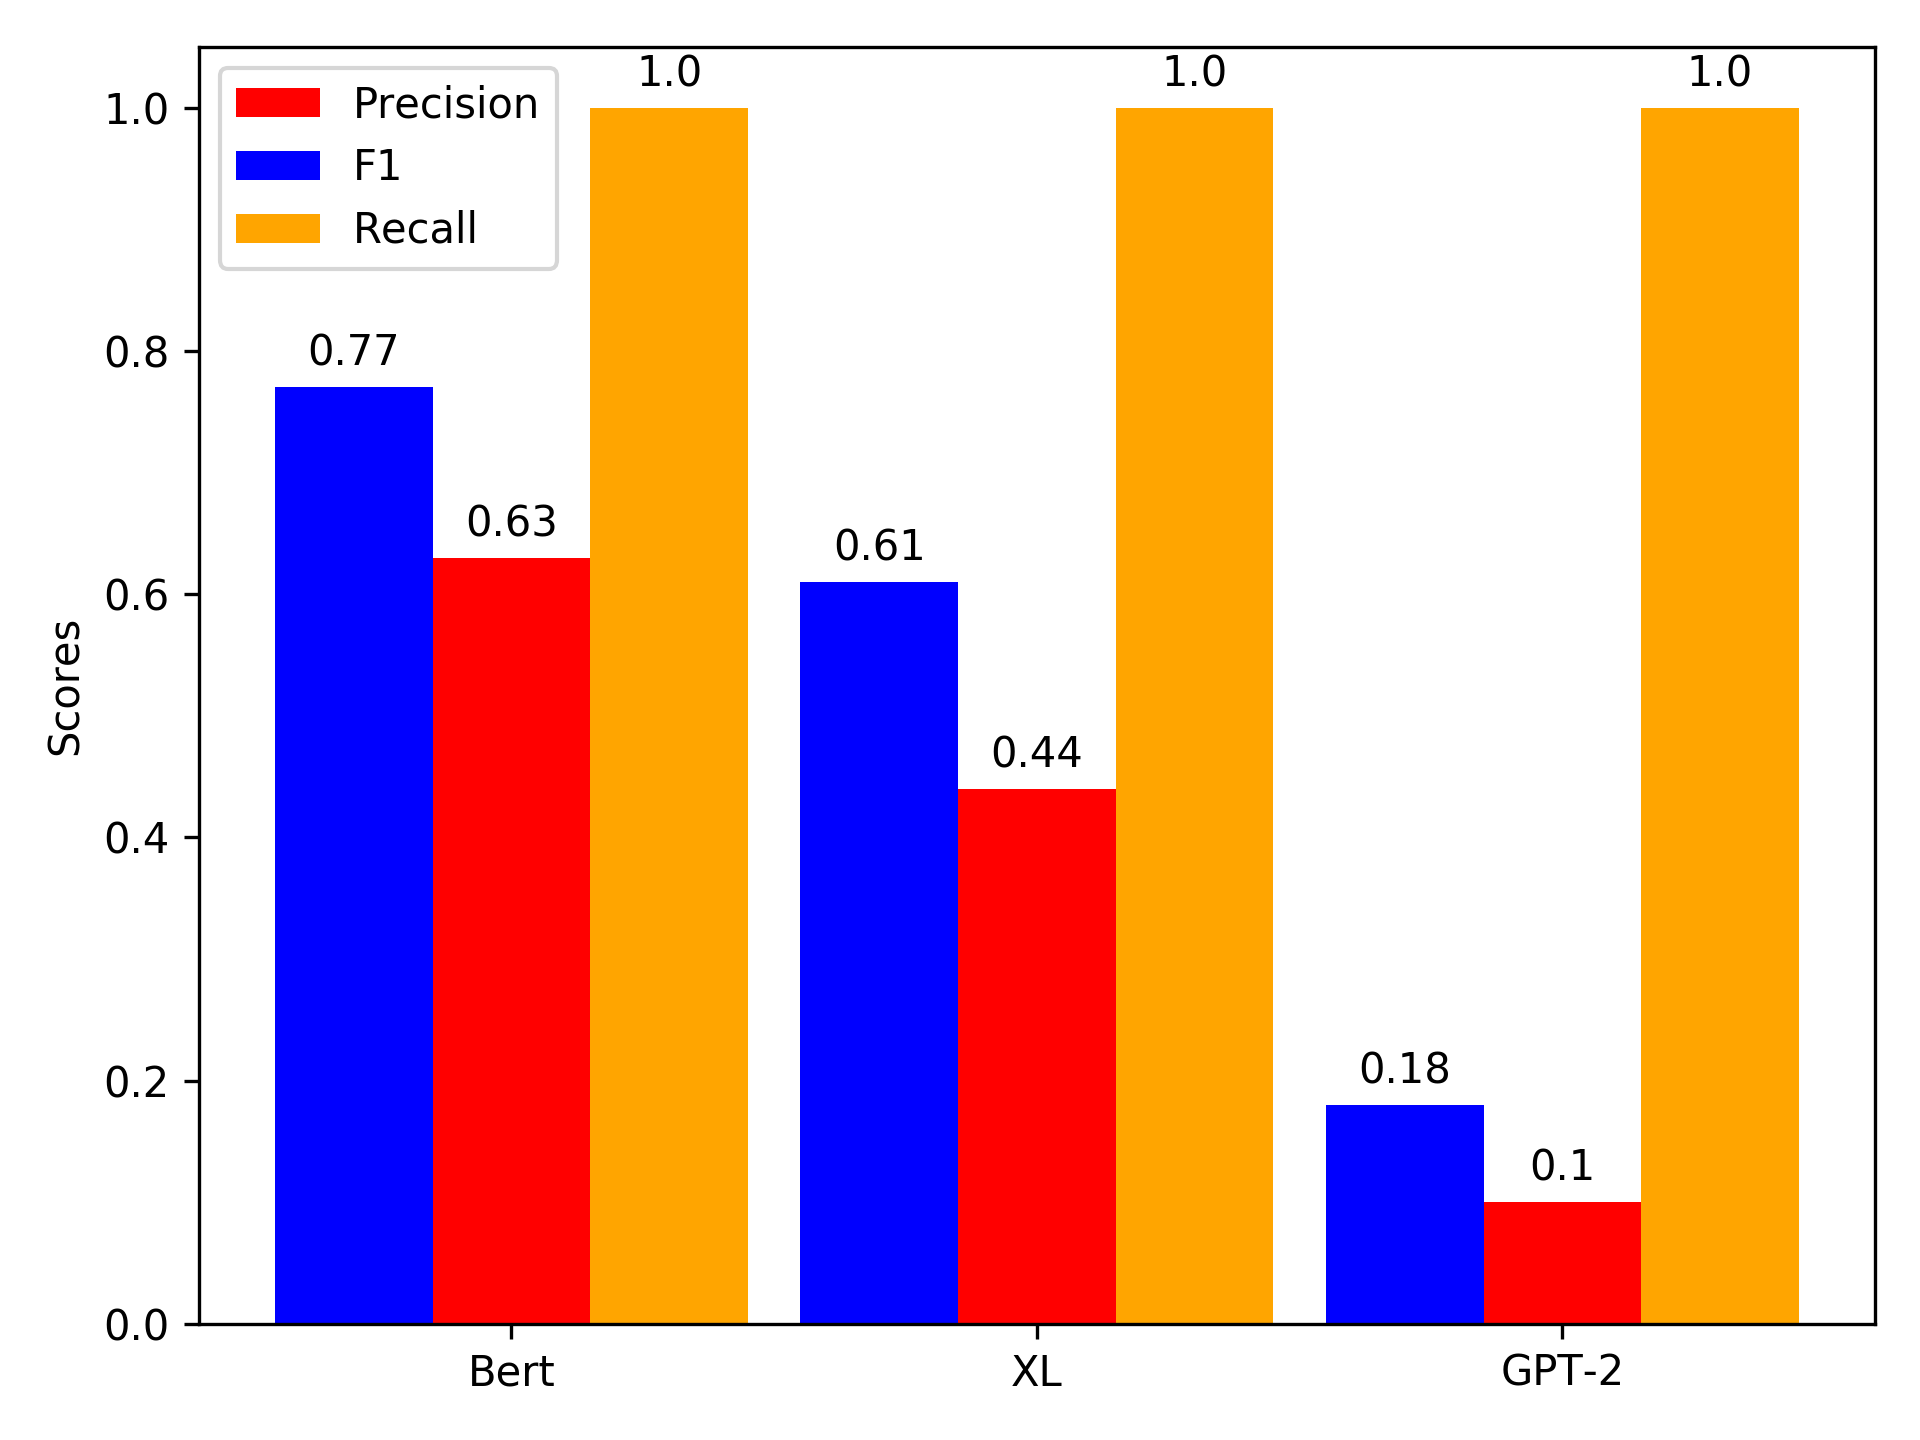
\includegraphics[trim={1cm 0.5cm 0cm 1cm}, width=0.322\textwidth]{results/transfer/transfer_multiclass_0.1_ratio.png}}
\hspace{\fill}
   \subfloat[15\% alteration\label{fig:results_transfer_classification_0.15}]{%
      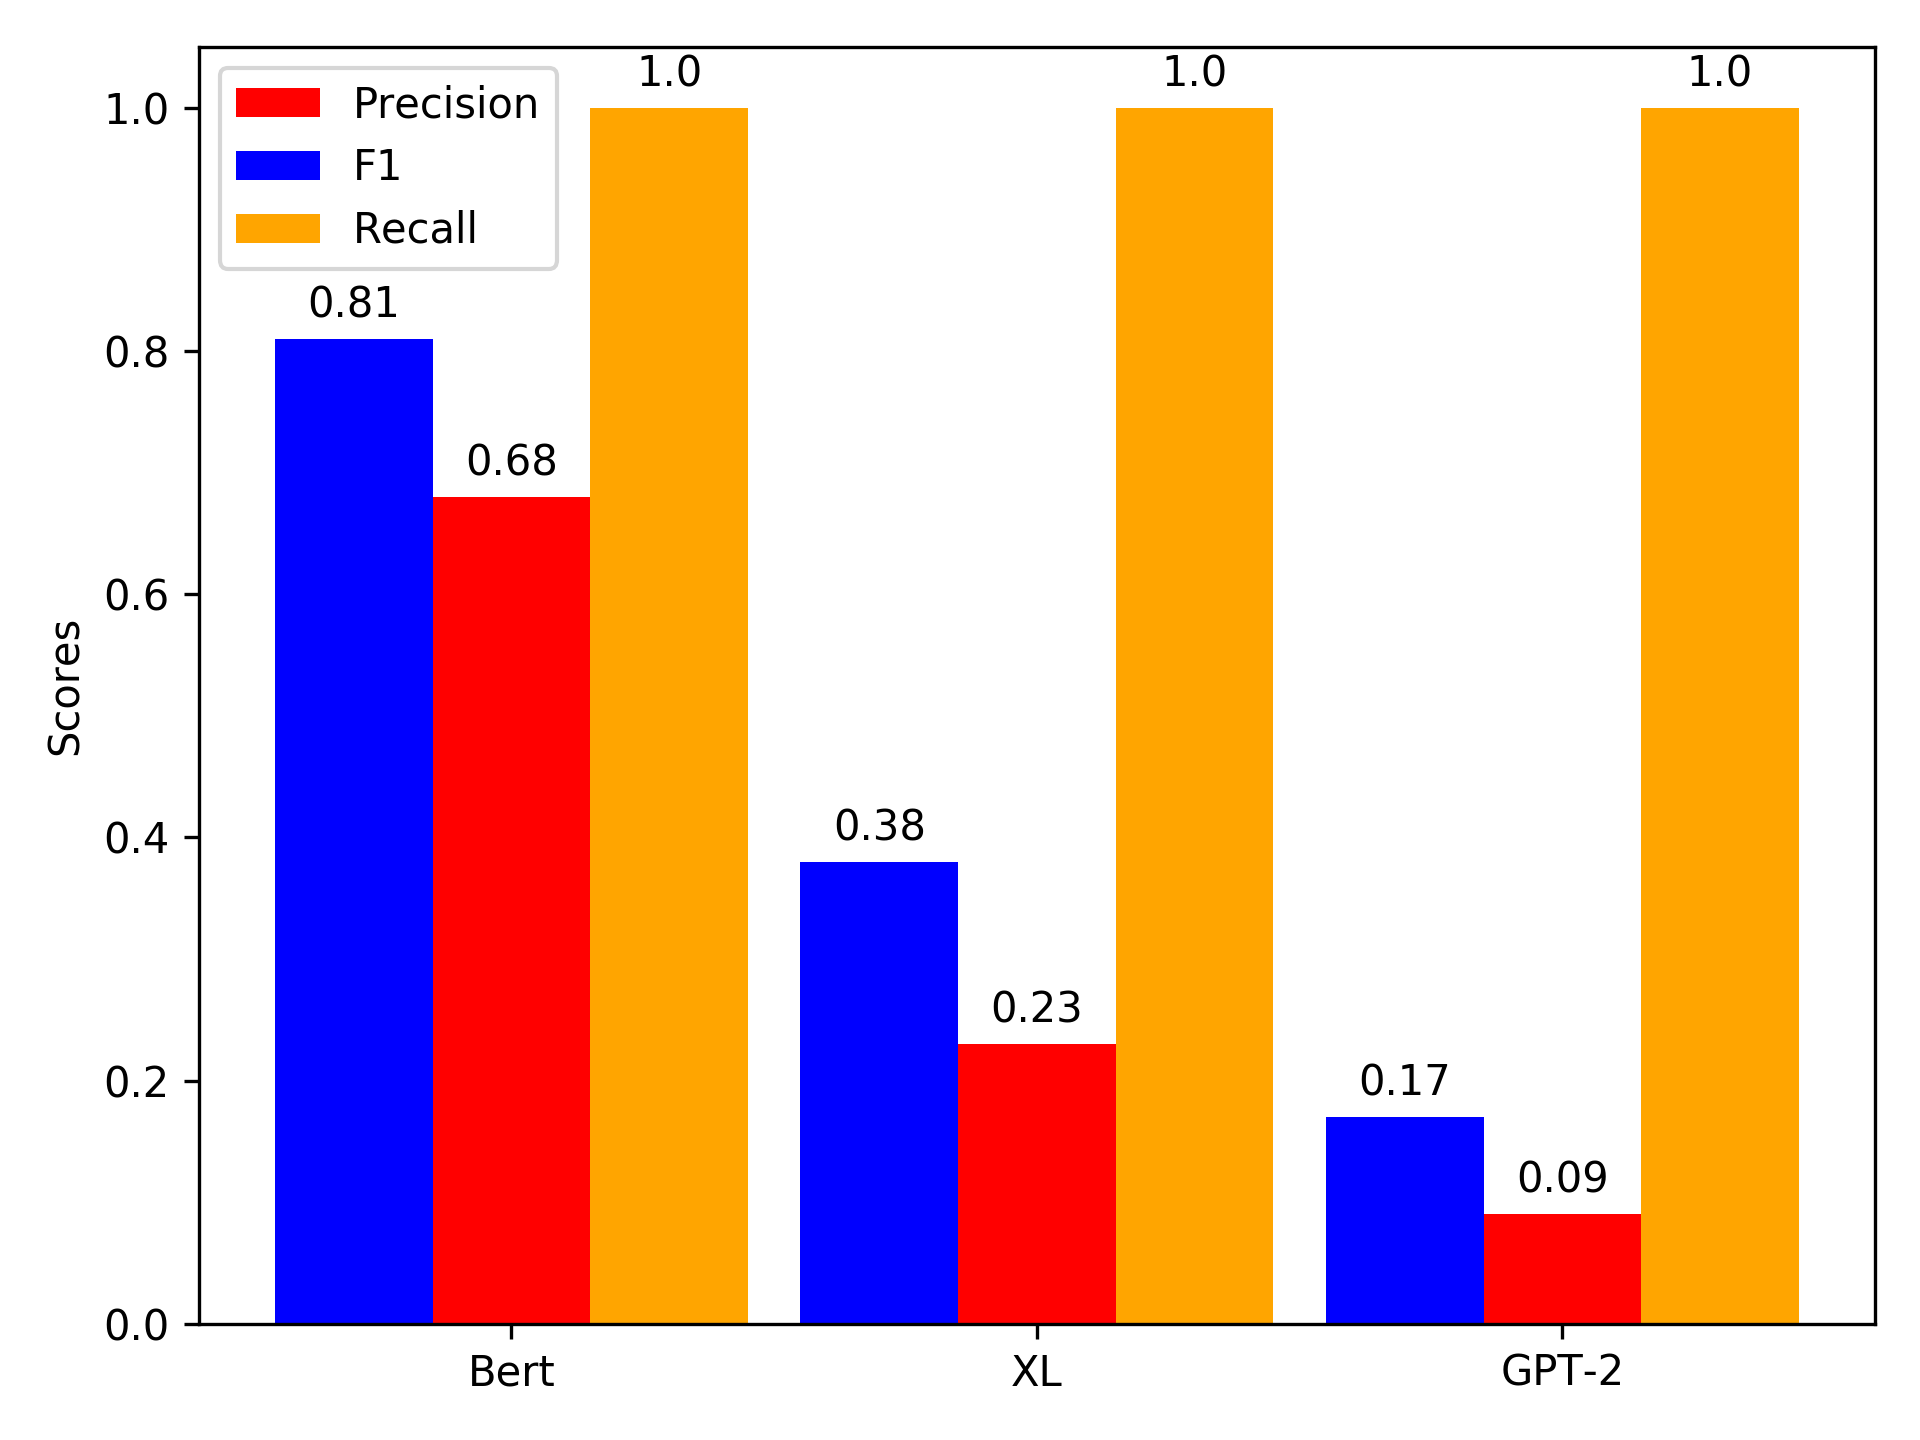
\includegraphics[trim={1cm 0.5cm 0cm 1cm}, width=0.322\textwidth]{results/transfer/transfer_multiclass_0.15_ratio.png}}\\
\caption{\label{fig:results_transfer_classification}Transfer learning with different ratios of alteration, using classification.}
\end{figure*}

\begin{figure*}[ht!]
   \subfloat[Bert\label{fig:results_transfer_multiclass_per_epoch_0.05}]{%
      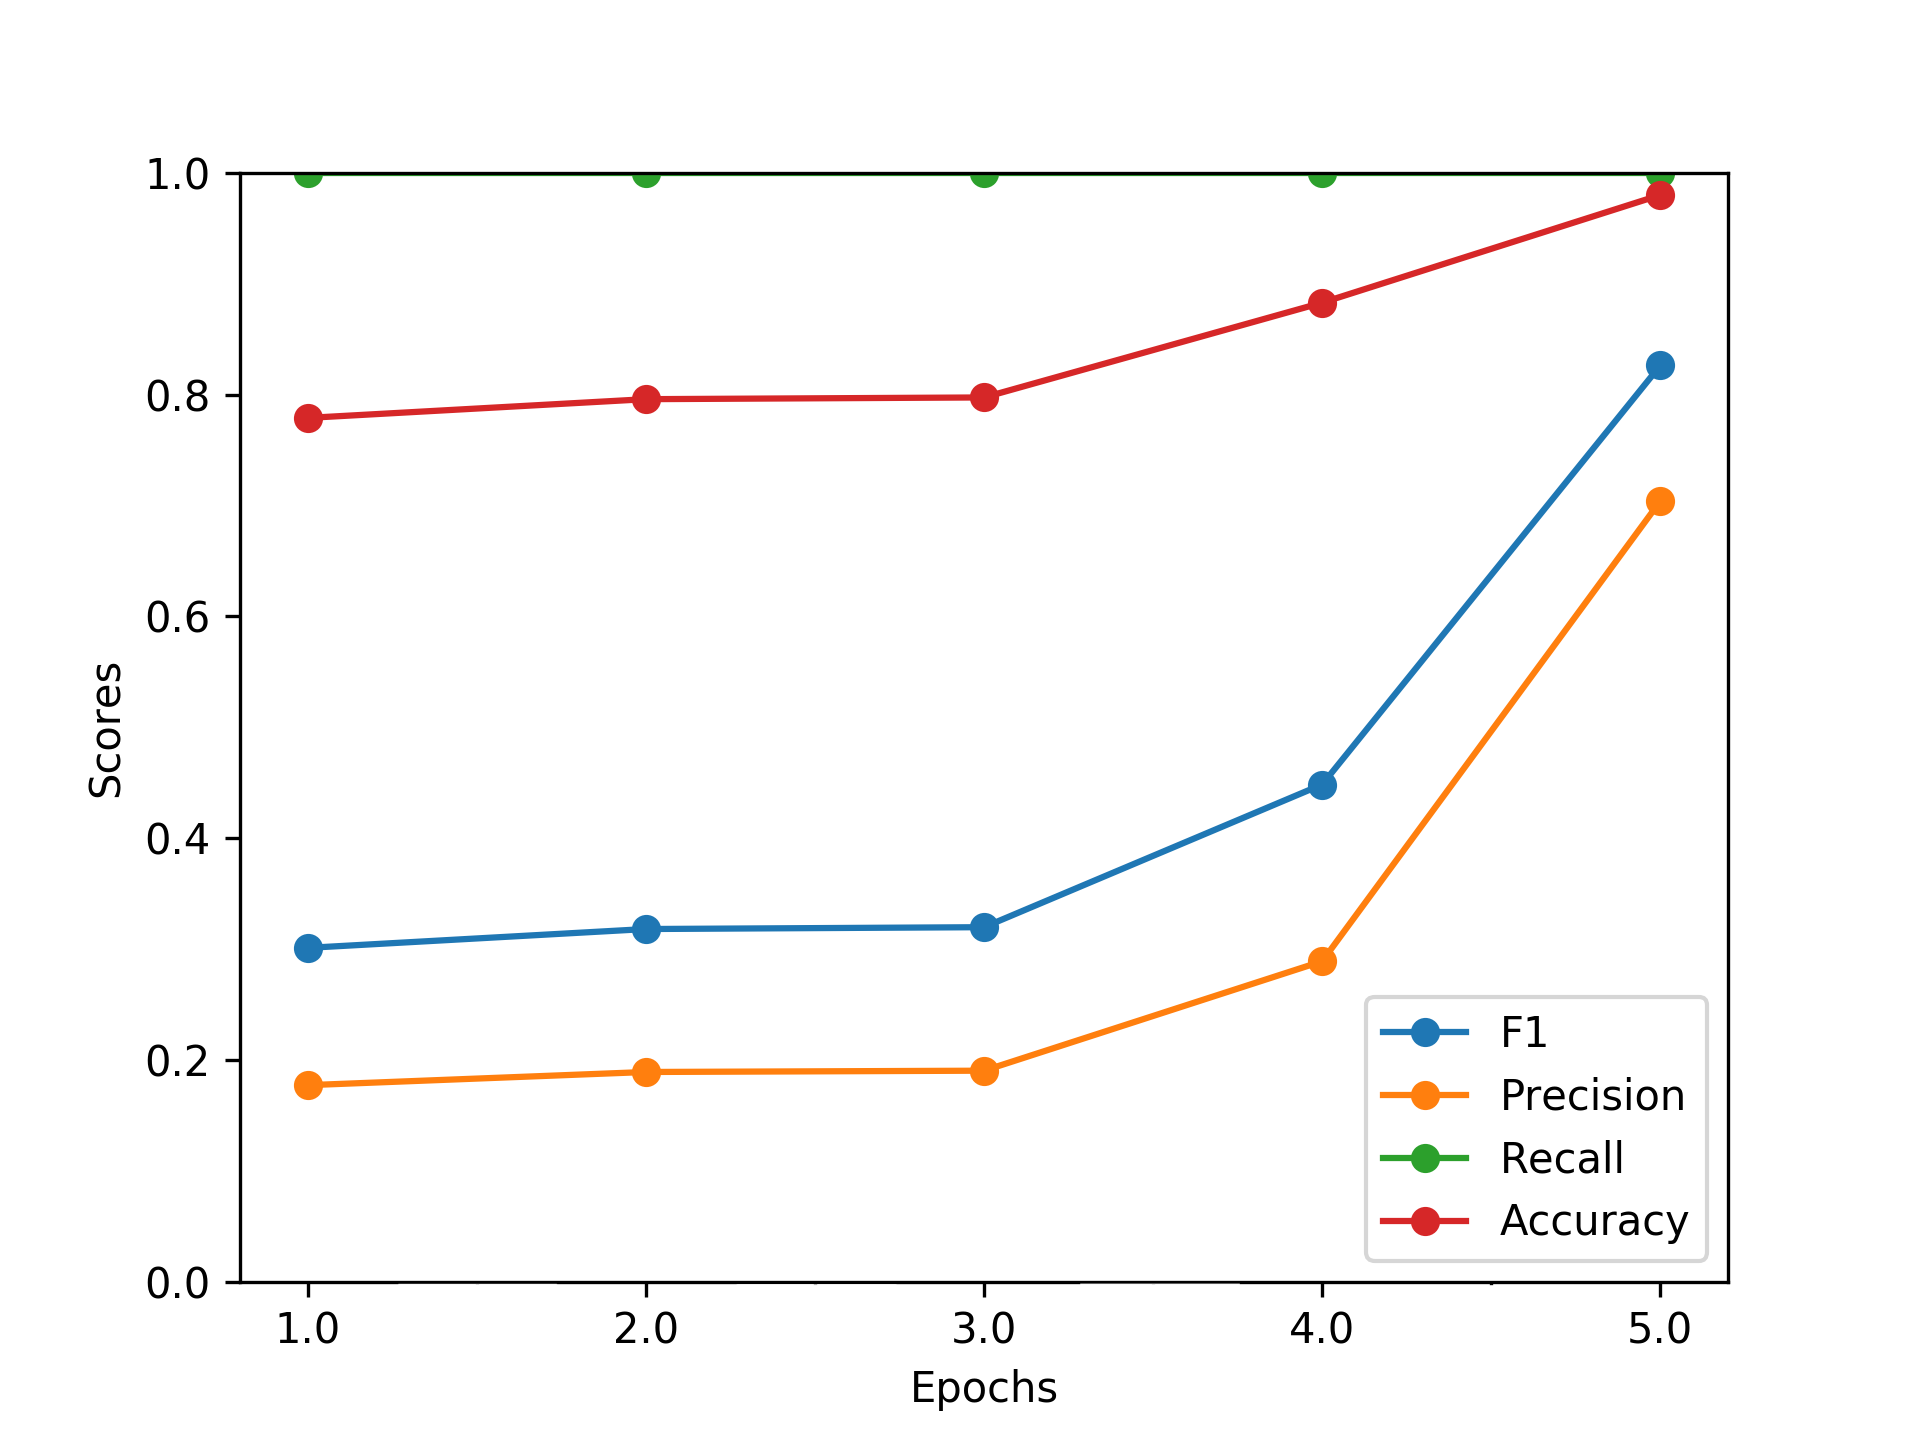
\includegraphics[trim={1cm 0.5cm 0cm 1cm}, width=0.322\textwidth]{results/transfer/bert_multiclass_0.15_transfer_metrics_per_epoch.png}}
\hspace{\fill}
   \subfloat[GPT-2\label{fig:results_transfer_multiclass_per_epoch_0.10} ]{%
      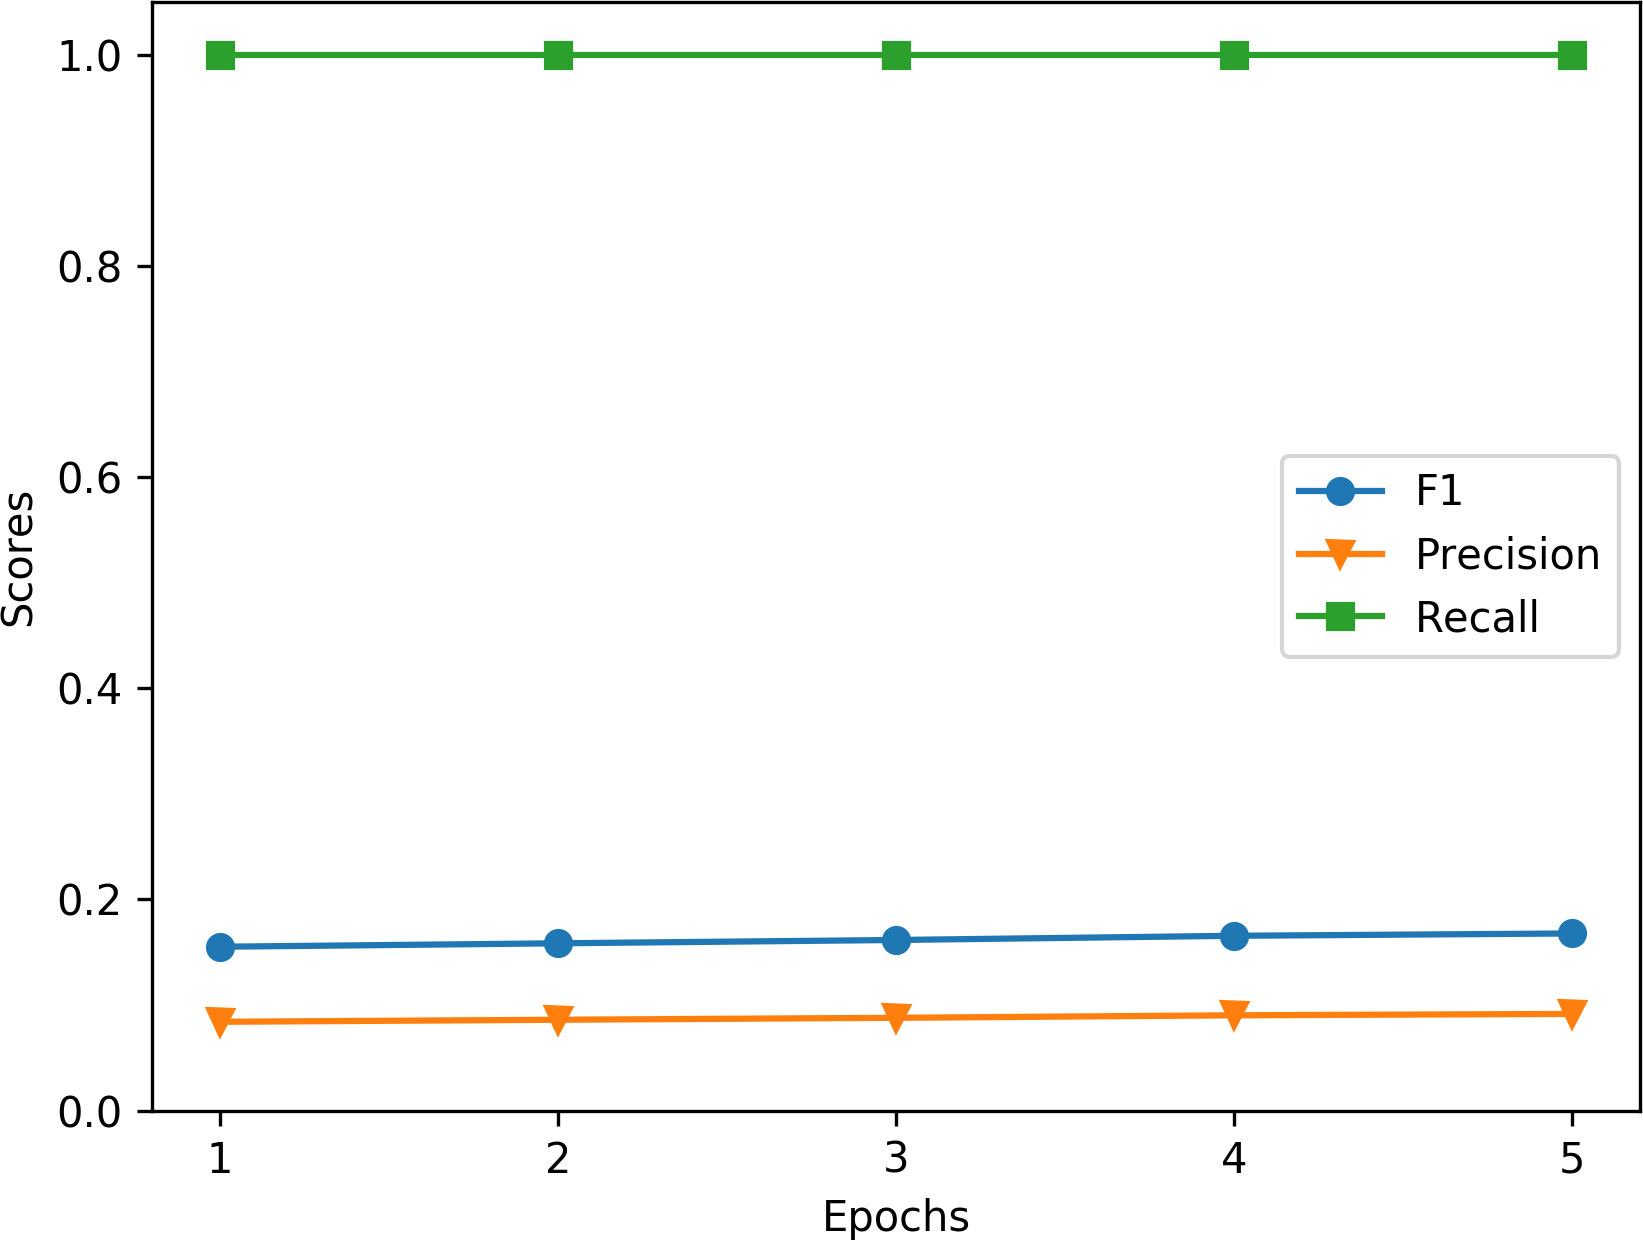
\includegraphics[trim={1cm 0.5cm 0cm 1cm}, width=0.322\textwidth]{results/transfer/gpt_multiclass_0.15_transfer_metrics_per_epoch.png}}
\hspace{\fill}
   \subfloat[XL\label{fig:results_transfer_multiclass_per_epoch_0.15}]{%
      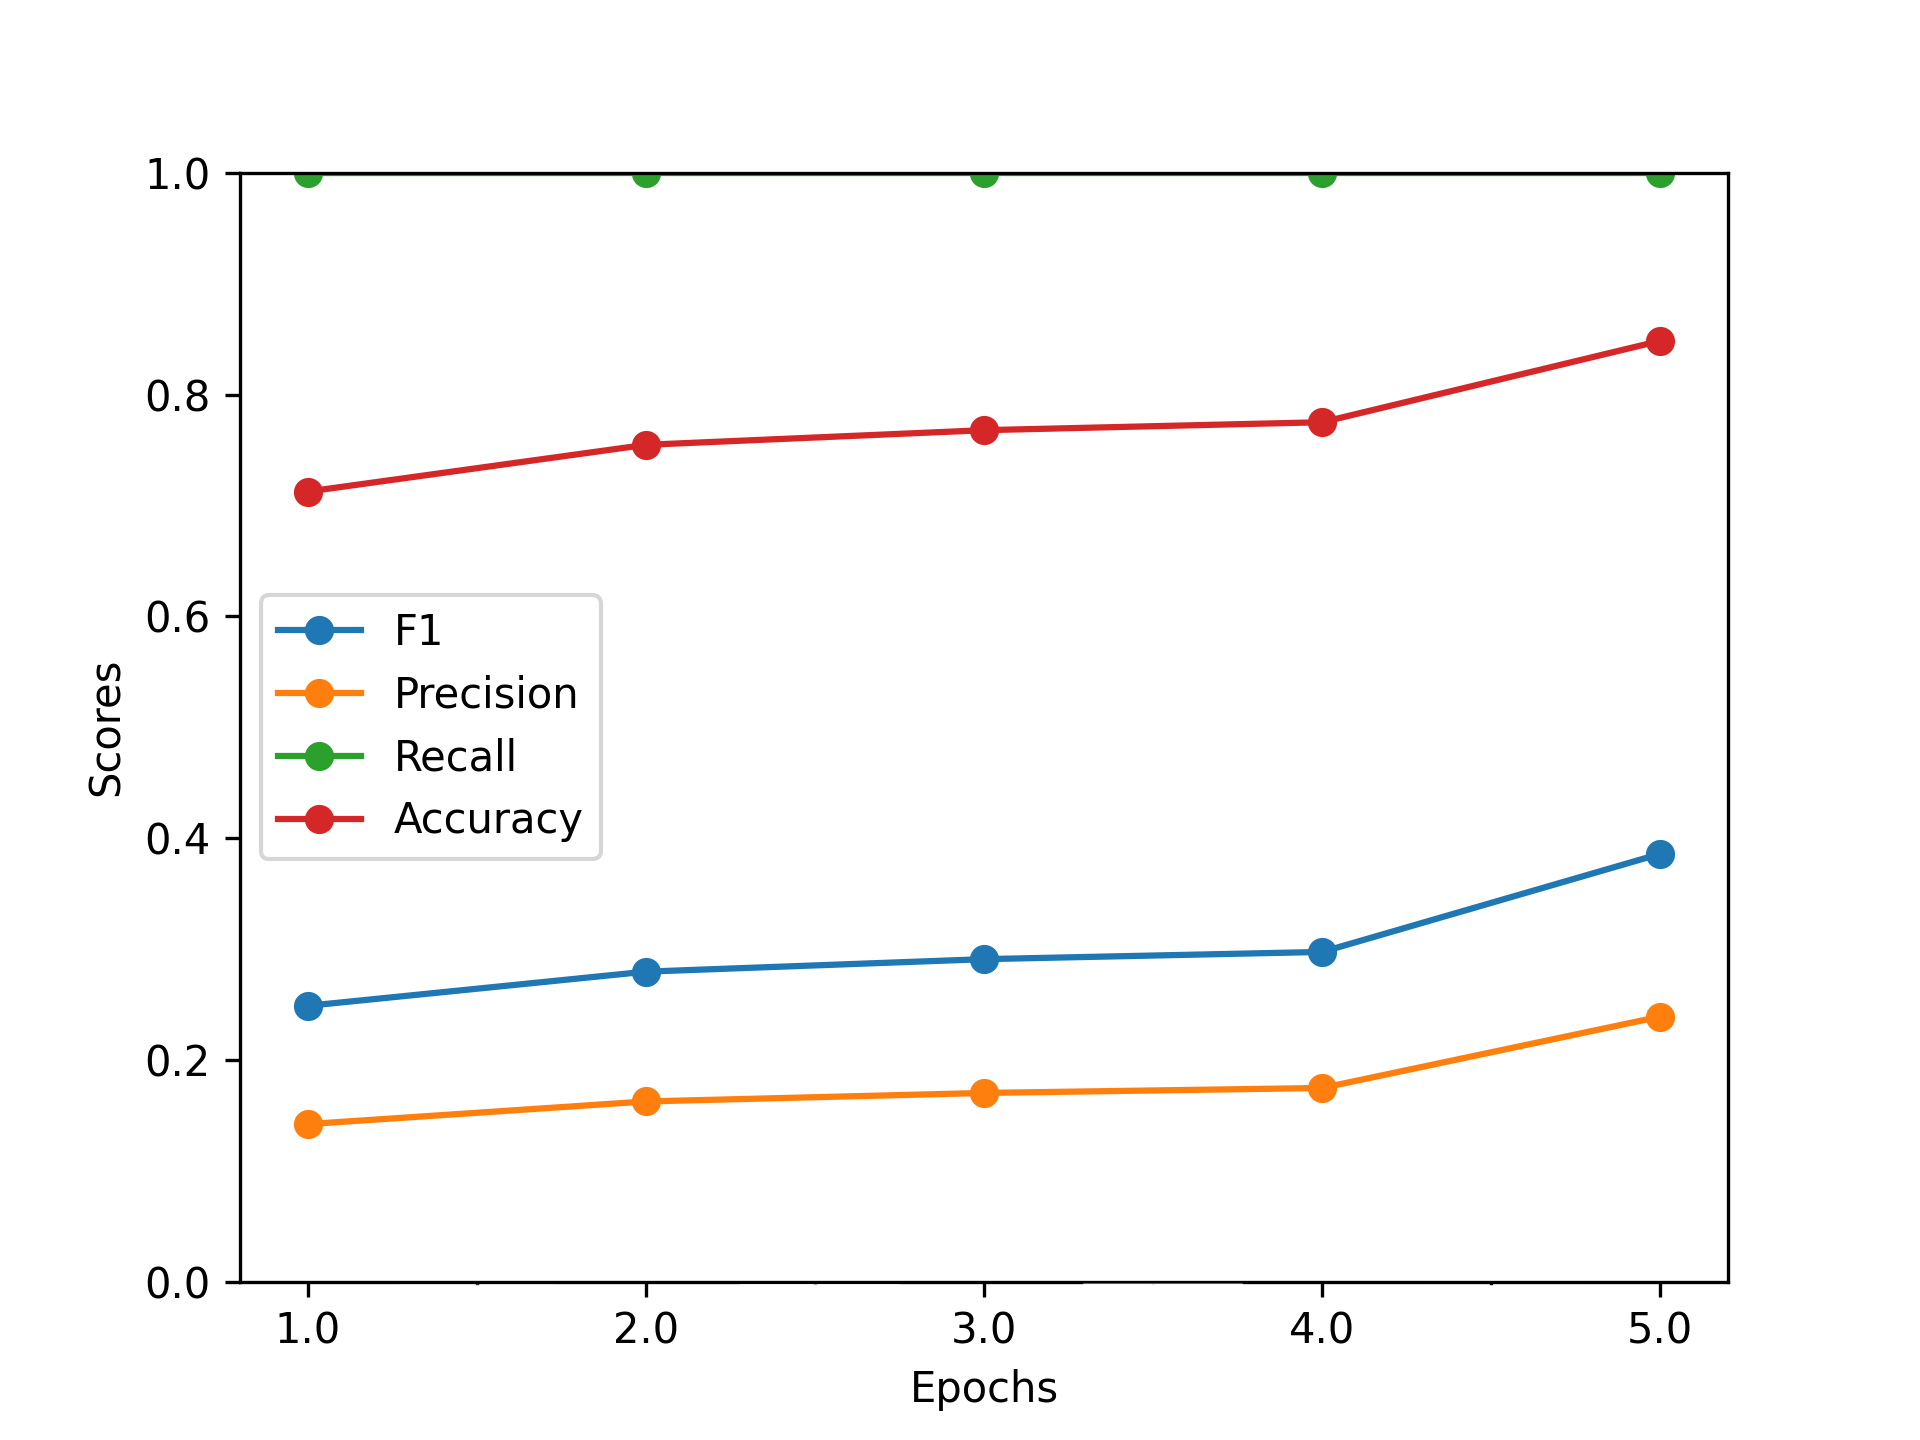
\includegraphics[trim={1cm 0.5cm 0cm 1cm}, width=0.322\textwidth]{results/transfer/xl_multiclass_0.15_transfer_metrics_per_epoch.png}}\\
\caption{\label{fig:results_transfer_multiclass_per_epoch}Improvement of metrics per additional learning epoch, using classification.}
\end{figure*}


\begin{figure*}[ht!]
   \subfloat[Bert\label{fig:roc_curve_bert_transfer_multiclass}]{%
      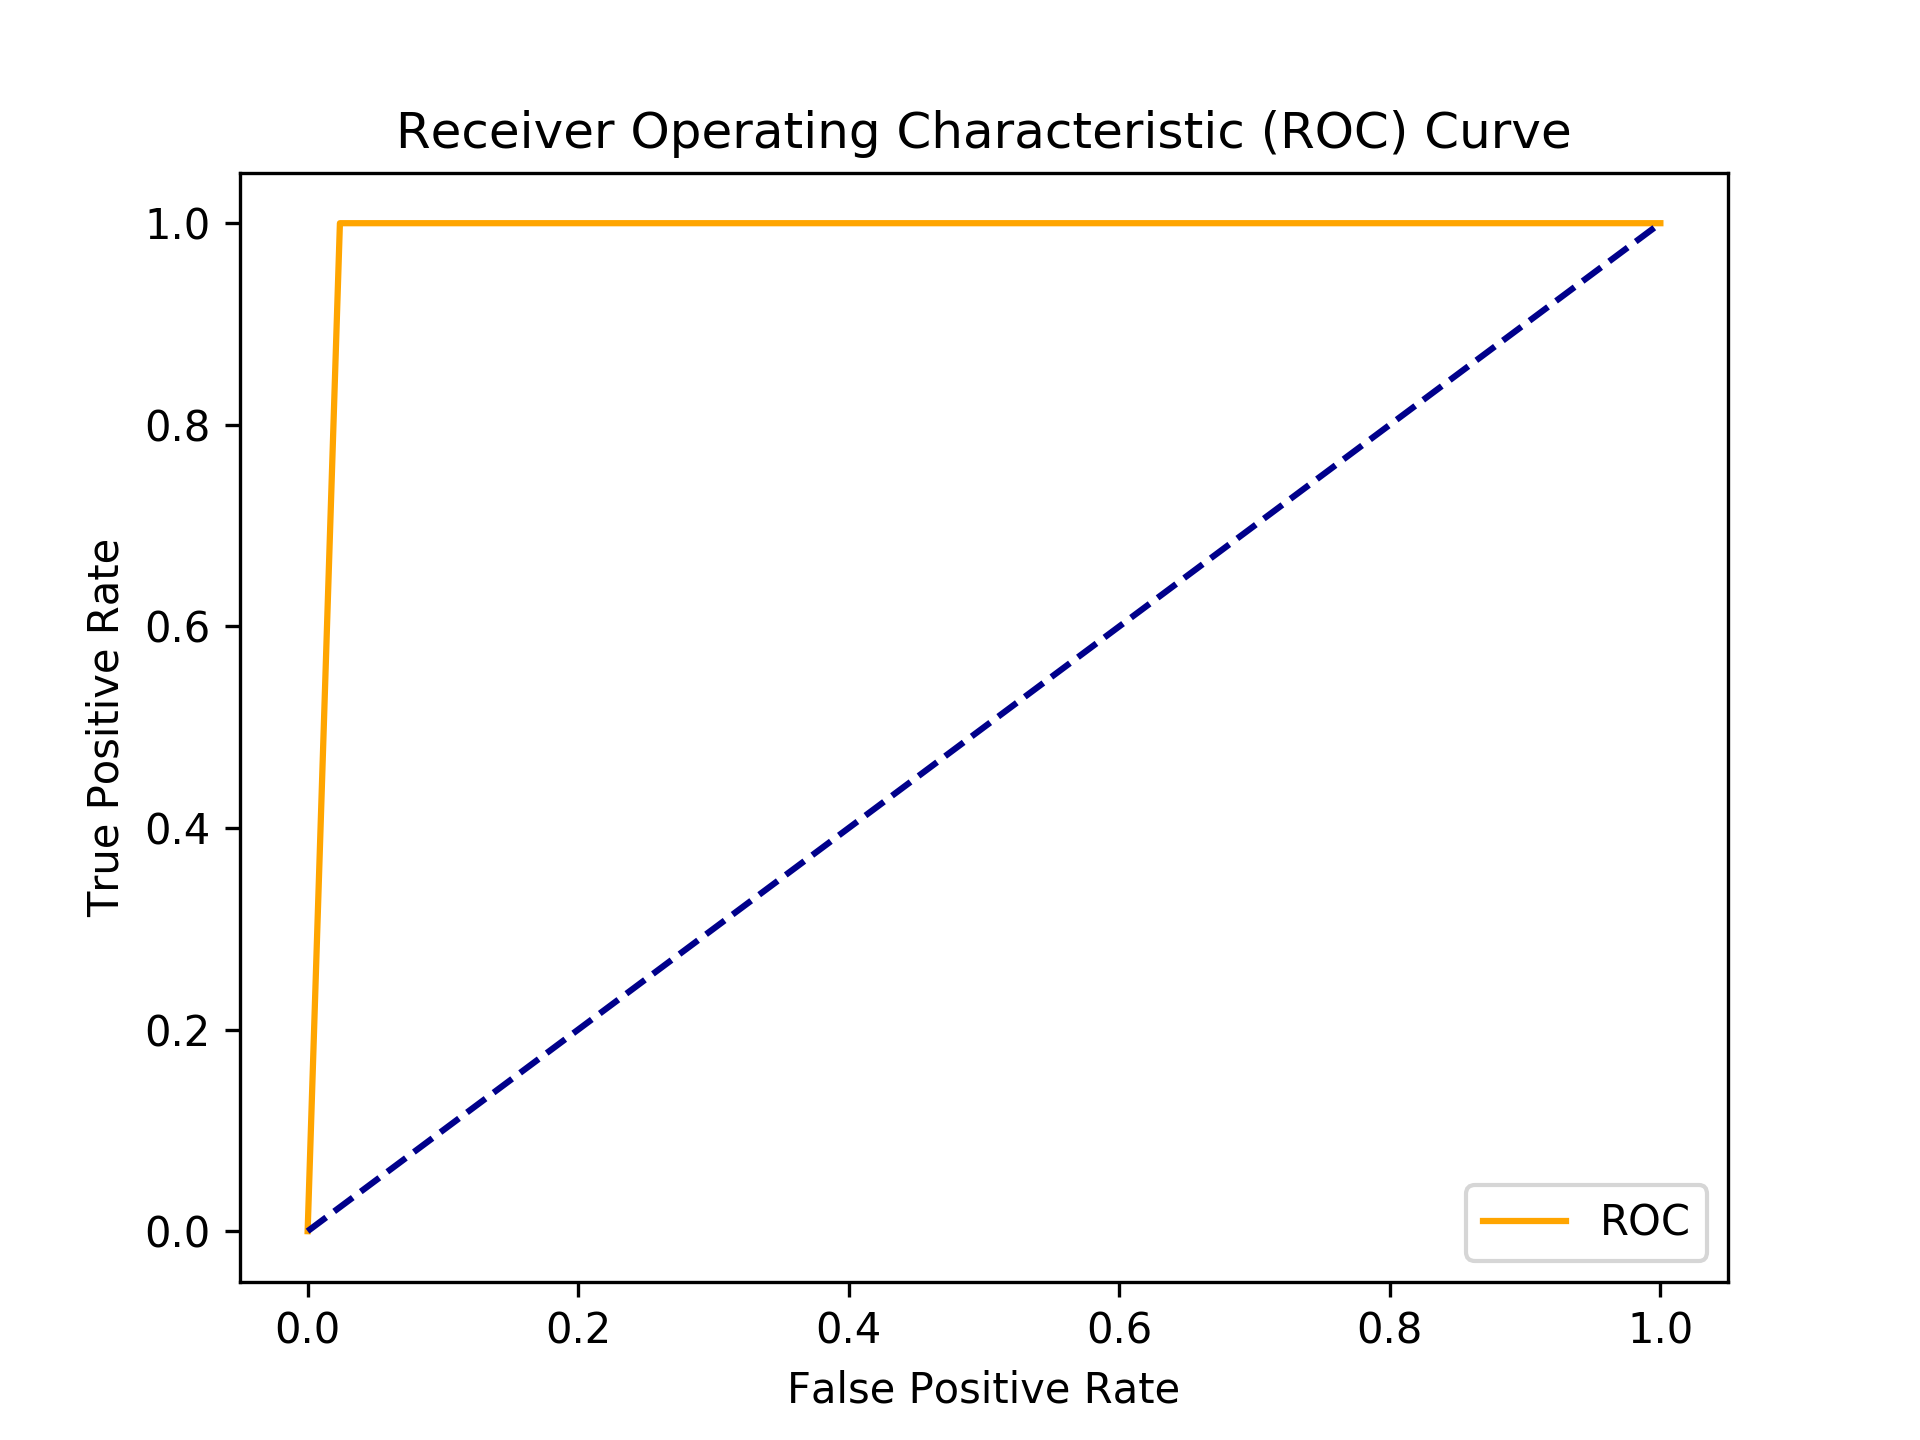
\includegraphics[trim={1cm 0.5cm 0cm 1cm}, width=0.322\textwidth]{results/transfer/roc_curve_transfer_multiclass_bert_0.15.png}}
\hspace{\fill}
   \subfloat[GPT-2\label{fig:roc_curve_gpt_transfer_multiclass} ]{%
      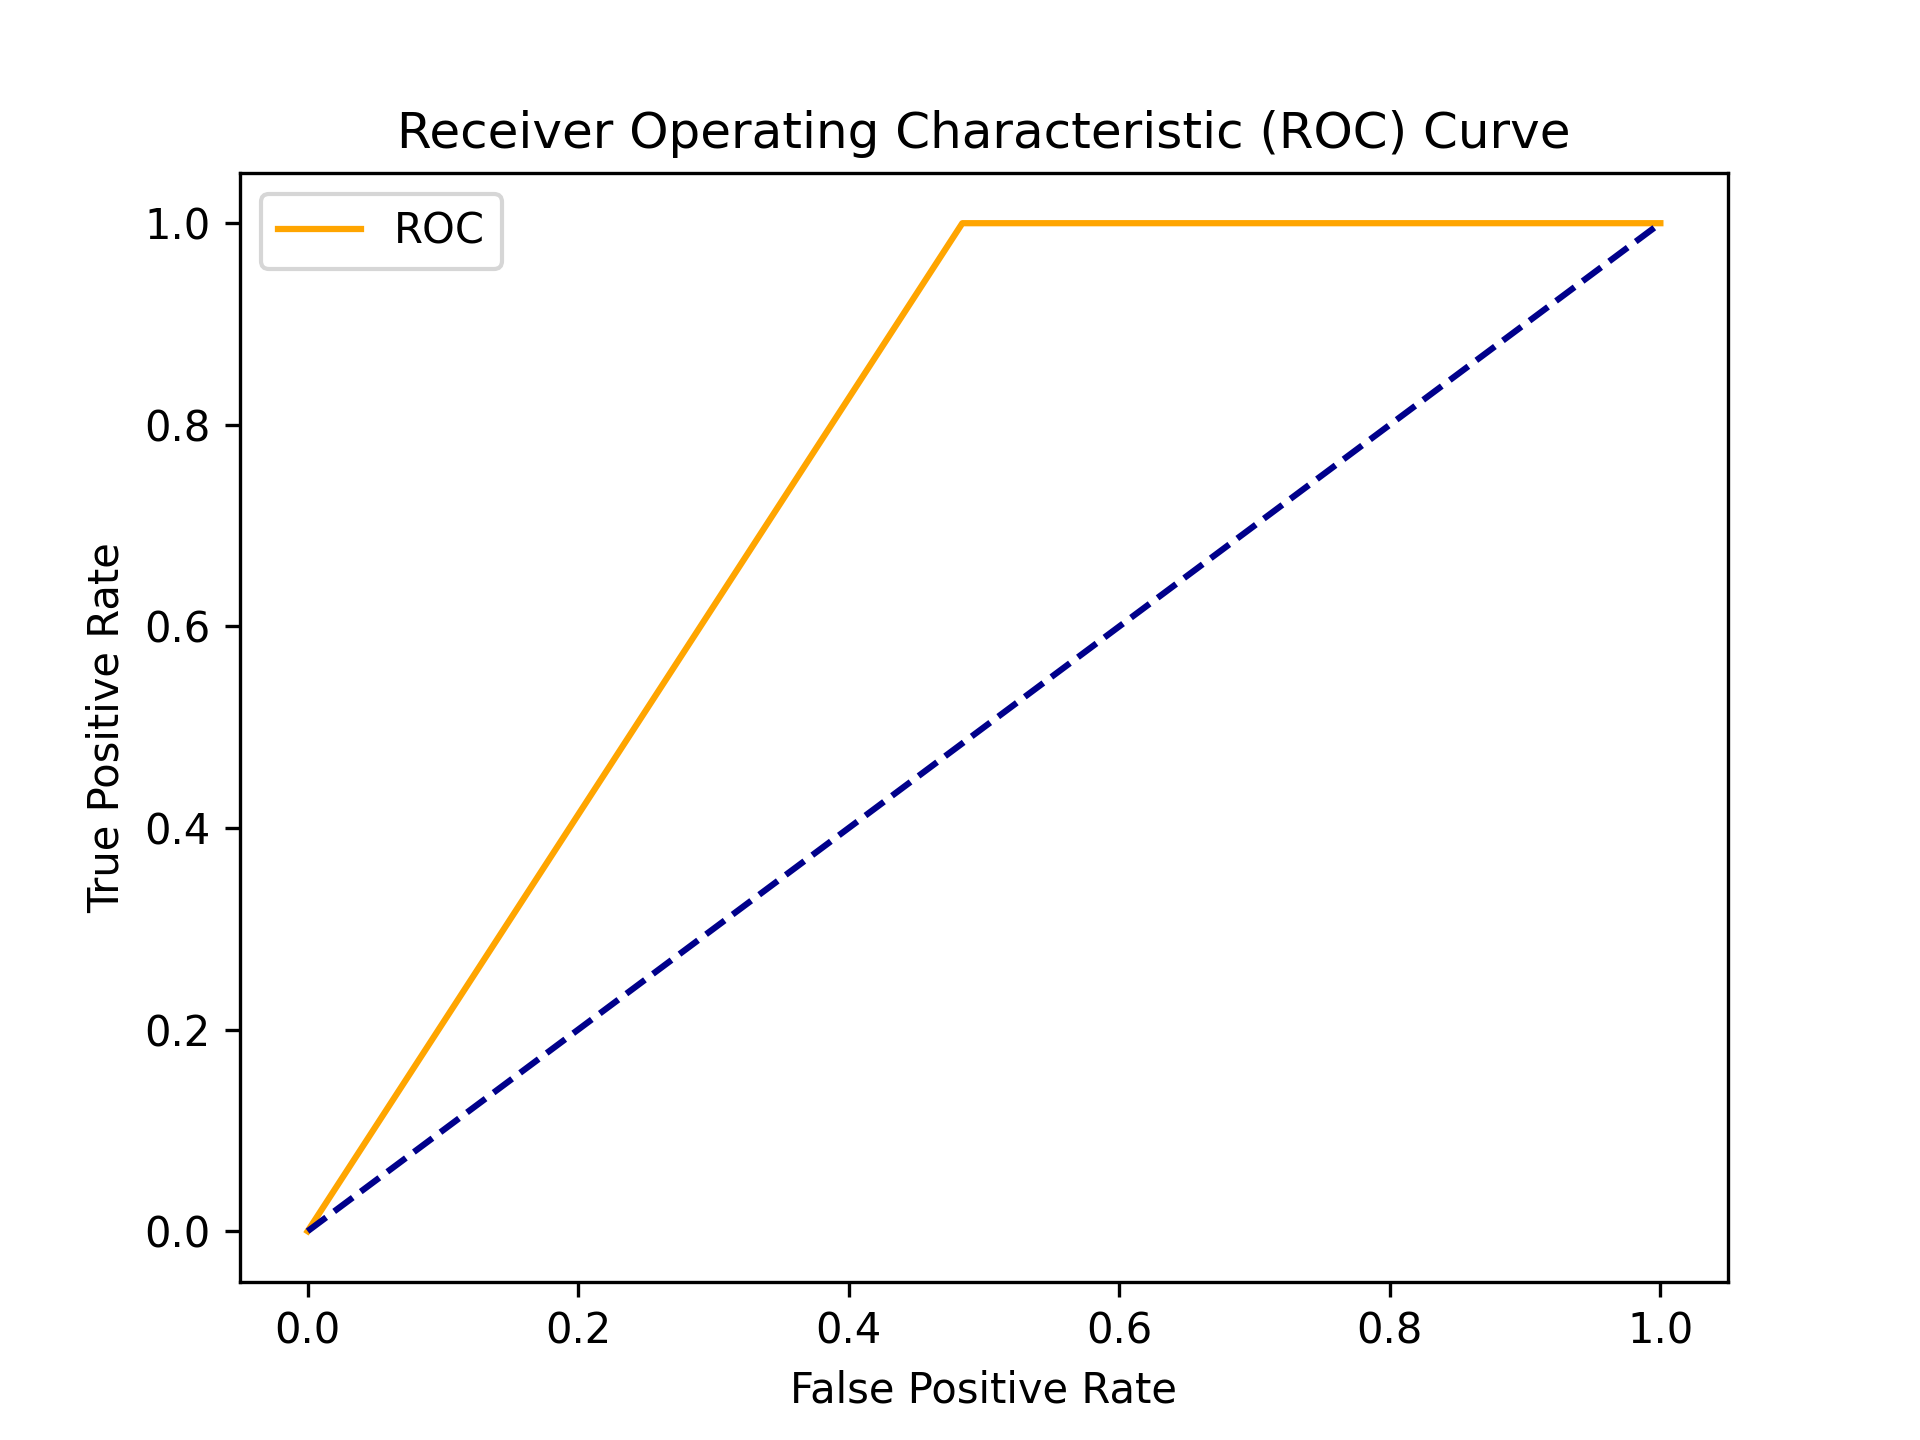
\includegraphics[trim={1cm 0.5cm 0cm 1cm}, width=0.322\textwidth]{results/transfer/roc_curve_transfer_multiclass_gpt_0.15.png}}
\hspace{\fill}
   \subfloat[XL\label{fig:roc_curve_xl_transfer_multiclass}]{%
      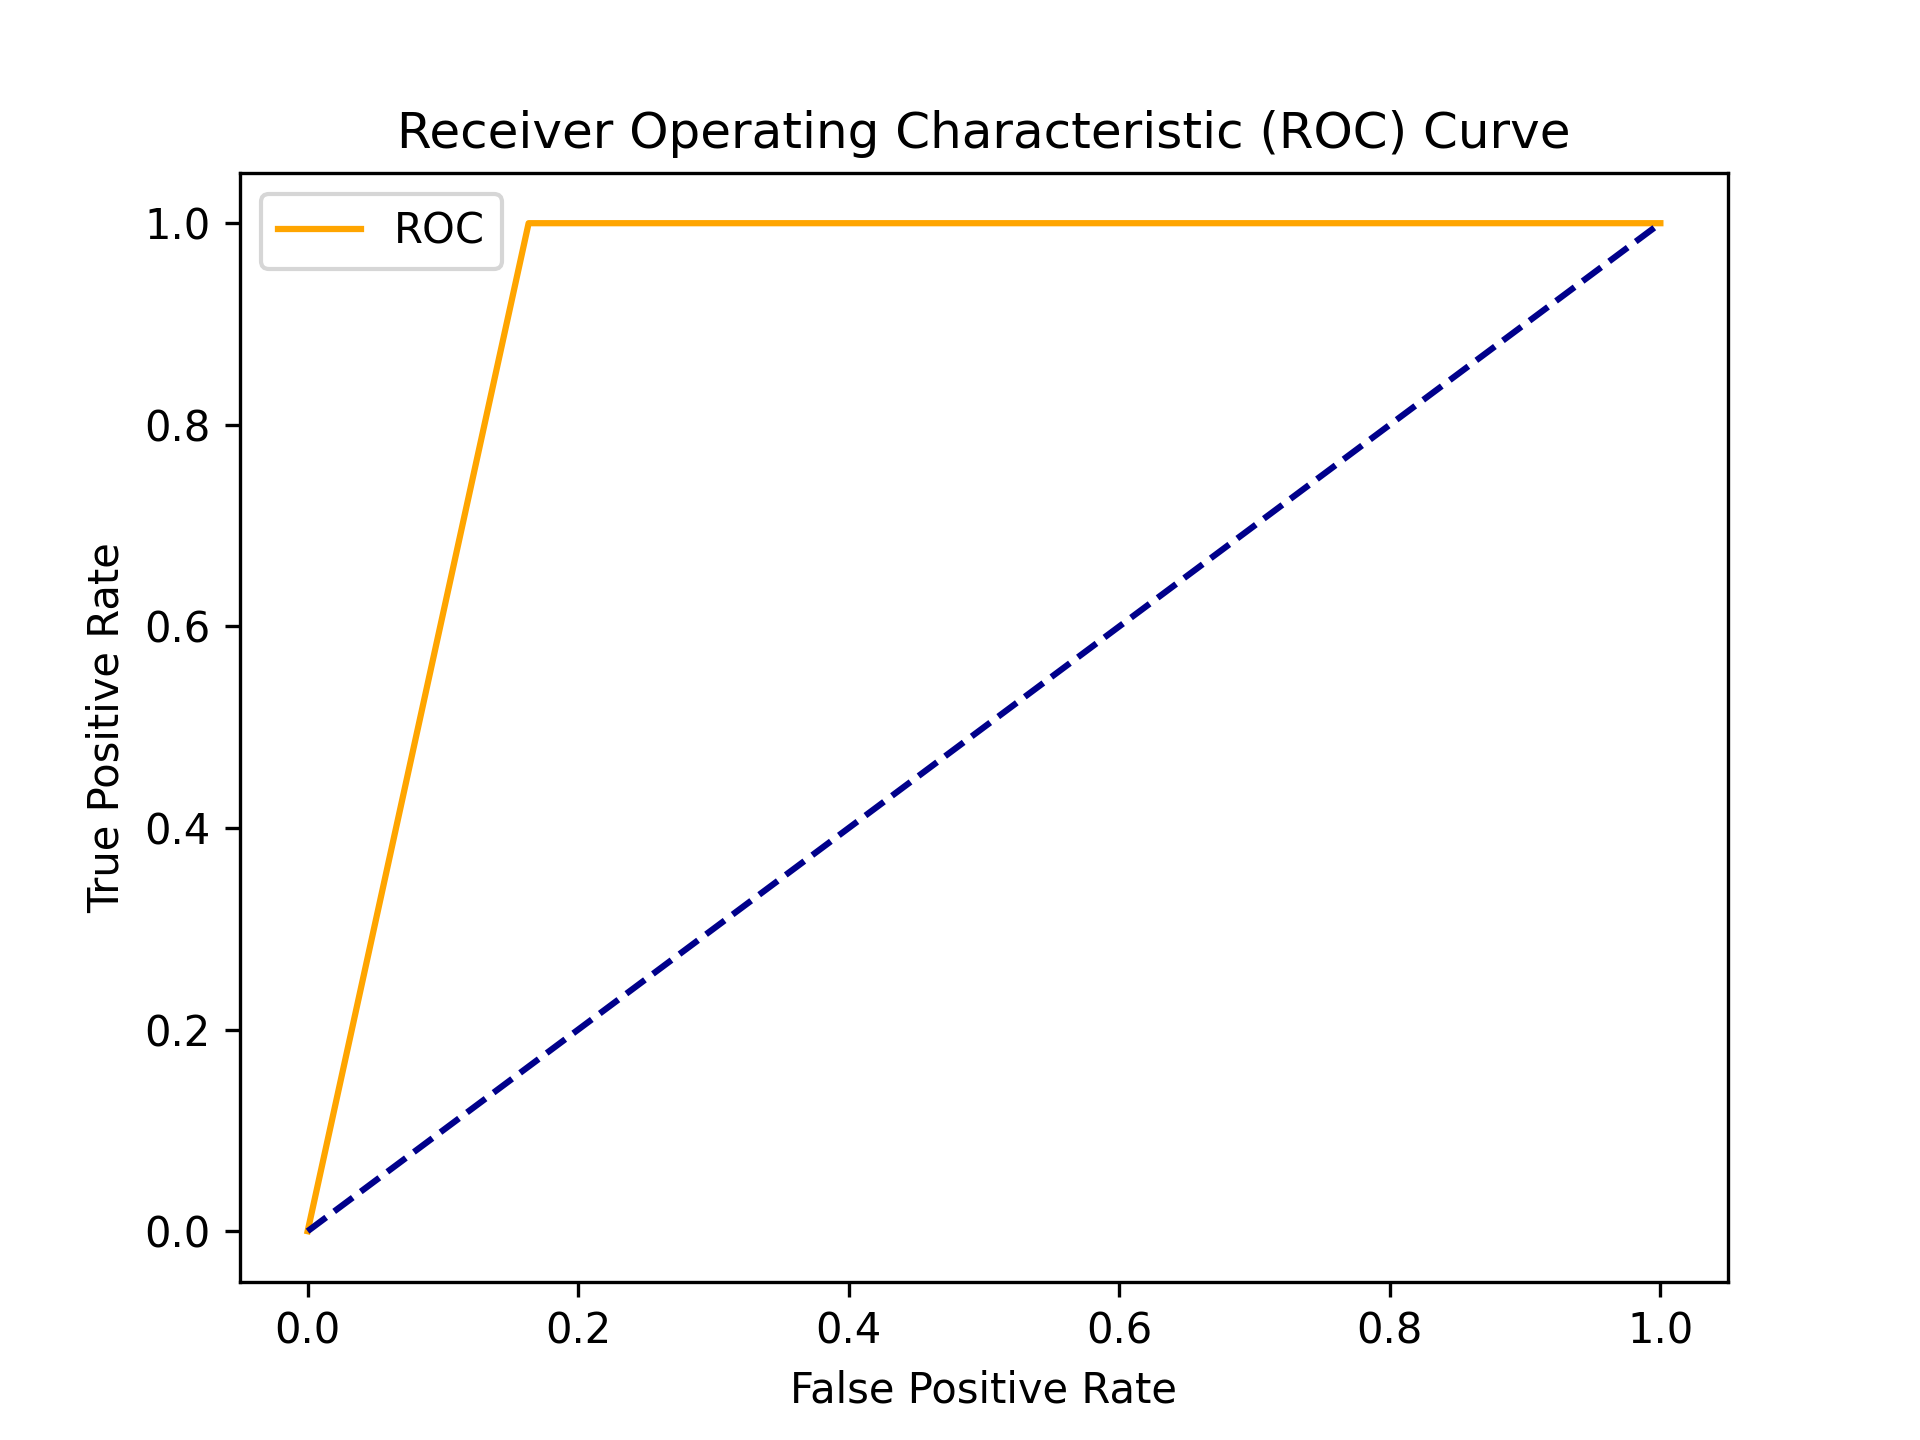
\includegraphics[trim={1cm 0.5cm 0cm 1cm}, width=0.322\textwidth]{results/transfer/roc_curve_transfer_multiclass_xl_0.15.png}}\\
\caption{\label{fig:results_transfer_multiclass_roc}ROC-Curve for transfer learning using regression with 15\% alterations.}
\end{figure*}



\section{Discussion of Results\label{sec:discussion_results}}
By evaluating three different language models, it has been shown that the used word embeddings can highly influence the quality of the results for anomaly detection, with different word embeddings having strengths and weaknesses in different categories. 

\begin{comment}
For anomaly detection on one dataset using the regression approach, GPT-2 shows strong results, with F1-Scores of 0.95 when altering 5\% of log sequences, and 0.93 when altering the log lines, the quality of the results don't degrade much, when alteration ratios are increased, where Bert and XL-Transformers show decreases of 0.1 to 0.2 percentage points when increasing the alteration ratio from 5\% to 15\%. Yet, when the log events are completely reversed, GPT-2 achieves an F1-Score of only 0.55, where Bert and XL achieve 0.98, almost perfectly detecting the wrong sequence of log events.
\end{comment}

For the regression approach on one dataset, GPT-2 beats the Bert and XL-Transformers clearly with regards to all metrics, doubts are risen, if it really learns sequences, when looking of the results of the reverse order experiment.

For the classification approach on one dataset on the other hand, GPT-2   shows weaker results than XL-Transformers and Bert. This is probably party due to the small cosine distance between the embeddings of the templates, where small changes on the templates can have a high impact already. Yet for the reverse order experiment, GPT-2 shows better results than the other two.

For the transfer learning approach, the results show a slightly different picture. Using the regression approach, GPT-2 is still ahead of the other two, while Bert seems to show better results than for detection on one dataset. 

On the other hand, for transfer learning using the classification-based approach, for 15\% alteration, GPT-2 shows results that are not much better than random, while still being able to find all anomalies, but showing a small F1-Score of only 0.17, where Bert is able to reach a F1-Score of 0.81. It is also visible, that GPT-2 seems to not profit as much from the few-show learning on dataset B, where the metrics stay almost the same throughout, yet Bert shows improvements from an F1-Score of 0.3 to 0.8.

It is evident, that with more hyperparameter-tuning, far better results can be accomplished, especially with XL-Transformers, since it obviously requires a different setup of hidden units and layers within the LSTM to achieve optimal results, however, since the model is a prototype and is supposed to show the possibility of comparing different word embeddings, not all potentials were fully tapped.

%TODO box plots of loss values in 